\documentclass[twoside]{book}

% Packages required by doxygen
\usepackage{fixltx2e}
\usepackage{calc}
\usepackage{doxygen}
\usepackage[export]{adjustbox} % also loads graphicx
\usepackage{graphicx}
\usepackage[utf8]{inputenc}
\usepackage{makeidx}
\usepackage{multicol}
\usepackage{multirow}
\PassOptionsToPackage{warn}{textcomp}
\usepackage{textcomp}
\usepackage[nointegrals]{wasysym}
\usepackage[table]{xcolor}

% Font selection
\usepackage[T1]{fontenc}
\usepackage[scaled=.90]{helvet}
\usepackage{courier}
\usepackage{amssymb}
\usepackage{sectsty}
\renewcommand{\familydefault}{\sfdefault}
\allsectionsfont{%
  \fontseries{bc}\selectfont%
  \color{darkgray}%
}
\renewcommand{\DoxyLabelFont}{%
  \fontseries{bc}\selectfont%
  \color{darkgray}%
}
\newcommand{\+}{\discretionary{\mbox{\scriptsize$\hookleftarrow$}}{}{}}

% Page & text layout
\usepackage{geometry}
\geometry{%
  a4paper,%
  top=2.5cm,%
  bottom=2.5cm,%
  left=2.5cm,%
  right=2.5cm%
}
\tolerance=750
\hfuzz=15pt
\hbadness=750
\setlength{\emergencystretch}{15pt}
\setlength{\parindent}{0cm}
\setlength{\parskip}{3ex plus 2ex minus 2ex}
\makeatletter
\renewcommand{\paragraph}{%
  \@startsection{paragraph}{4}{0ex}{-1.0ex}{1.0ex}{%
    \normalfont\normalsize\bfseries\SS@parafont%
  }%
}
\renewcommand{\subparagraph}{%
  \@startsection{subparagraph}{5}{0ex}{-1.0ex}{1.0ex}{%
    \normalfont\normalsize\bfseries\SS@subparafont%
  }%
}
\makeatother

% Headers & footers
\usepackage{fancyhdr}
\pagestyle{fancyplain}
\fancyhead[LE]{\fancyplain{}{\bfseries\thepage}}
\fancyhead[CE]{\fancyplain{}{}}
\fancyhead[RE]{\fancyplain{}{\bfseries\leftmark}}
\fancyhead[LO]{\fancyplain{}{\bfseries\rightmark}}
\fancyhead[CO]{\fancyplain{}{}}
\fancyhead[RO]{\fancyplain{}{\bfseries\thepage}}
\fancyfoot[LE]{\fancyplain{}{}}
\fancyfoot[CE]{\fancyplain{}{}}
\fancyfoot[RE]{\fancyplain{}{\bfseries\scriptsize Generated by Doxygen }}
\fancyfoot[LO]{\fancyplain{}{\bfseries\scriptsize Generated by Doxygen }}
\fancyfoot[CO]{\fancyplain{}{}}
\fancyfoot[RO]{\fancyplain{}{}}
\renewcommand{\footrulewidth}{0.4pt}
\renewcommand{\chaptermark}[1]{%
  \markboth{#1}{}%
}
\renewcommand{\sectionmark}[1]{%
  \markright{\thesection\ #1}%
}

% Indices & bibliography
\usepackage{natbib}
\usepackage[titles]{tocloft}
\setcounter{tocdepth}{3}
\setcounter{secnumdepth}{5}
\makeindex

% Hyperlinks (required, but should be loaded last)
\usepackage{ifpdf}
\ifpdf
  \usepackage[pdftex,pagebackref=true]{hyperref}
\else
  \usepackage[ps2pdf,pagebackref=true]{hyperref}
\fi
\hypersetup{%
  colorlinks=true,%
  linkcolor=blue,%
  citecolor=blue,%
  unicode%
}

% Custom commands
\newcommand{\clearemptydoublepage}{%
  \newpage{\pagestyle{empty}\cleardoublepage}%
}

\usepackage{caption}
\captionsetup{labelsep=space,justification=centering,font={bf},singlelinecheck=off,skip=4pt,position=top}

%===== C O N T E N T S =====

\begin{document}

% Titlepage & ToC
\hypersetup{pageanchor=false,
             bookmarksnumbered=true,
             pdfencoding=unicode
            }
\pagenumbering{alph}
\begin{titlepage}
\vspace*{7cm}
\begin{center}%
{\Large OS Project \\[1ex]\large 1 }\\
\vspace*{1cm}
{\large Generated by Doxygen 1.8.14}\\
\end{center}
\end{titlepage}
\clearemptydoublepage
\pagenumbering{roman}
\tableofcontents
\clearemptydoublepage
\pagenumbering{arabic}
\hypersetup{pageanchor=true}

%--- Begin generated contents ---
\chapter{Namespace Index}
\section{Namespace List}
Here is a list of all documented namespaces with brief descriptions\+:\begin{DoxyCompactList}
\item\contentsline{section}{\mbox{\hyperlink{namespacecore}{core}} \\*This namespace contains the core part of the project, everything about disk }{\pageref{namespacecore}}{}
\item\contentsline{section}{\mbox{\hyperlink{namespacecore_1_1disk}{core\+::disk}} \\*This namespace contains the disk part of each disk }{\pageref{namespacecore_1_1disk}}{}
\item\contentsline{section}{\mbox{\hyperlink{namespacecore_1_1logic}{core\+::logic}} \\*This namespace contains the logic part of each disk }{\pageref{namespacecore_1_1logic}}{}
\item\contentsline{section}{\mbox{\hyperlink{namespaceui}{ui}} \\*This namespace contains all ui elements for this project }{\pageref{namespaceui}}{}
\item\contentsline{section}{\mbox{\hyperlink{namespaceui_1_1custom_u_i}{ui\+::custom\+UI}} \\*This namespace contains all custom implementation of UI elements }{\pageref{namespaceui_1_1custom_u_i}}{}
\item\contentsline{section}{\mbox{\hyperlink{namespaceui_1_1window}{ui\+::window}} \\*This namespace contains all windows for this project }{\pageref{namespaceui_1_1window}}{}
\item\contentsline{section}{\mbox{\hyperlink{namespaceui_1_1wizard}{ui\+::wizard}} \\*This namespace contains all wizards for this project }{\pageref{namespaceui_1_1wizard}}{}
\item\contentsline{section}{\mbox{\hyperlink{namespaceui_1_1wizard_1_1pages}{ui\+::wizard\+::pages}} \\*This namespace contains all wizard pages for this project }{\pageref{namespaceui_1_1wizard_1_1pages}}{}
\end{DoxyCompactList}

\chapter{Hierarchical Index}
\section{Class Hierarchy}
This inheritance list is sorted roughly, but not completely, alphabetically\+:\begin{DoxyCompactList}
\item \contentsline{section}{A\+PI}{\pageref{class_a_p_i}}{}
\item \contentsline{section}{core\+:\+:logic\+:\+:Block}{\pageref{classcore_1_1logic_1_1_block}}{}
\item \contentsline{section}{core\+:\+:disk\+:\+:Disk}{\pageref{classcore_1_1disk_1_1_disk}}{}
\item \contentsline{section}{core\+:\+:I\+File\+System}{\pageref{classcore_1_1_i_file_system}}{}
\item \contentsline{section}{core\+:\+:disk\+:\+:Master\+Boot\+Record}{\pageref{classcore_1_1disk_1_1_master_boot_record}}{}
\item \contentsline{section}{core\+:\+:logic\+:\+:Partition}{\pageref{classcore_1_1logic_1_1_partition}}{}
\item Q\+List\+Widget\+Item\begin{DoxyCompactList}
\item \contentsline{section}{ui\+:\+:custom\+UI\+:\+:Custom\+List\+Widget\+Item}{\pageref{classui_1_1custom_u_i_1_1_custom_list_widget_item}}{}
\end{DoxyCompactList}
\item Q\+Object\begin{DoxyCompactList}
\item \contentsline{section}{ui\+:\+:window\+:\+:Detail\+Page}{\pageref{classui_1_1window_1_1_detail_page}}{}
\end{DoxyCompactList}
\item Q\+Push\+Button\begin{DoxyCompactList}
\item \contentsline{section}{ui\+:\+:custom\+UI\+:\+:Custom\+Control\+Bar}{\pageref{classui_1_1custom_u_i_1_1_custom_control_bar}}{}
\end{DoxyCompactList}
\item Q\+Widget\begin{DoxyCompactList}
\item \contentsline{section}{ui\+:\+:window\+:\+:Disk\+Info}{\pageref{classui_1_1window_1_1_disk_info}}{}
\item \contentsline{section}{ui\+:\+:window\+:\+:Main\+Window}{\pageref{classui_1_1window_1_1_main_window}}{}
\item \contentsline{section}{ui\+:\+:window\+:\+:Resize\+Partition}{\pageref{classui_1_1window_1_1_resize_partition}}{}
\end{DoxyCompactList}
\item Q\+Wizard\begin{DoxyCompactList}
\item \contentsline{section}{ui\+:\+:wizard\+:\+:Disk\+Wizard}{\pageref{classui_1_1wizard_1_1_disk_wizard}}{}
\item \contentsline{section}{ui\+:\+:wizard\+:\+:Partition\+Wizard}{\pageref{classui_1_1wizard_1_1_partition_wizard}}{}
\end{DoxyCompactList}
\item Q\+Wizard\+Page\begin{DoxyCompactList}
\item \contentsline{section}{ui\+:\+:wizard\+:\+:pages\+:\+:Disk\+Page}{\pageref{classui_1_1wizard_1_1pages_1_1_disk_page}}{}
\item \contentsline{section}{ui\+:\+:wizard\+:\+:pages\+:\+:Intro\+Page}{\pageref{classui_1_1wizard_1_1pages_1_1_intro_page}}{}
\item \contentsline{section}{ui\+:\+:wizard\+:\+:pages\+:\+:Partition\+Page}{\pageref{classui_1_1wizard_1_1pages_1_1_partition_page}}{}
\item \contentsline{section}{ui\+:\+:wizard\+:\+:pages\+:\+:Summary\+Page}{\pageref{classui_1_1wizard_1_1pages_1_1_summary_page}}{}
\end{DoxyCompactList}
\end{DoxyCompactList}

\chapter{Class Index}
\section{Class List}
Here are the classes, structs, unions and interfaces with brief descriptions\+:\begin{DoxyCompactList}
\item\contentsline{section}{\mbox{\hyperlink{class_a_p_i}{A\+PI}} }{\pageref{class_a_p_i}}{}
\item\contentsline{section}{\mbox{\hyperlink{classcore_1_1logic_1_1_block}{core\+::logic\+::\+Block}} \\*The \mbox{\hyperlink{classcore_1_1logic_1_1_block}{Block}} class }{\pageref{classcore_1_1logic_1_1_block}}{}
\item\contentsline{section}{\mbox{\hyperlink{classui_1_1custom_u_i_1_1_custom_control_bar}{ui\+::custom\+U\+I\+::\+Custom\+Control\+Bar}} \\*This class will be removed }{\pageref{classui_1_1custom_u_i_1_1_custom_control_bar}}{}
\item\contentsline{section}{\mbox{\hyperlink{classui_1_1custom_u_i_1_1_custom_list_widget_item}{ui\+::custom\+U\+I\+::\+Custom\+List\+Widget\+Item}} \\*This class This class provides a custom impelemntation of a Listwidget }{\pageref{classui_1_1custom_u_i_1_1_custom_list_widget_item}}{}
\item\contentsline{section}{\mbox{\hyperlink{classui_1_1window_1_1_detail_page}{ui\+::window\+::\+Detail\+Page}} \\*This class handles all new created windows }{\pageref{classui_1_1window_1_1_detail_page}}{}
\item\contentsline{section}{\mbox{\hyperlink{classcore_1_1disk_1_1_disk}{core\+::disk\+::\+Disk}} \\*The \mbox{\hyperlink{classcore_1_1disk_1_1_disk}{Disk}} class }{\pageref{classcore_1_1disk_1_1_disk}}{}
\item\contentsline{section}{\mbox{\hyperlink{classui_1_1window_1_1_disk_info}{ui\+::window\+::\+Disk\+Info}} \\*This class provides a disk info window }{\pageref{classui_1_1window_1_1_disk_info}}{}
\item\contentsline{section}{\mbox{\hyperlink{classui_1_1wizard_1_1pages_1_1_disk_page}{ui\+::wizard\+::pages\+::\+Disk\+Page}} \\*This class provides a custom implementation of a wizard page }{\pageref{classui_1_1wizard_1_1pages_1_1_disk_page}}{}
\item\contentsline{section}{\mbox{\hyperlink{classui_1_1wizard_1_1_disk_wizard}{ui\+::wizard\+::\+Disk\+Wizard}} \\*This class this class implements a wizard }{\pageref{classui_1_1wizard_1_1_disk_wizard}}{}
\item\contentsline{section}{\mbox{\hyperlink{classcore_1_1_i_file_system}{core\+::\+I\+File\+System}} }{\pageref{classcore_1_1_i_file_system}}{}
\item\contentsline{section}{\mbox{\hyperlink{classui_1_1wizard_1_1pages_1_1_intro_page}{ui\+::wizard\+::pages\+::\+Intro\+Page}} \\*This class provides a custom implementation of a wizard page }{\pageref{classui_1_1wizard_1_1pages_1_1_intro_page}}{}
\item\contentsline{section}{\mbox{\hyperlink{classui_1_1window_1_1_main_window}{ui\+::window\+::\+Main\+Window}} \\*The \mbox{\hyperlink{classui_1_1window_1_1_main_window}{Main\+Window}} class }{\pageref{classui_1_1window_1_1_main_window}}{}
\item\contentsline{section}{\mbox{\hyperlink{classcore_1_1disk_1_1_master_boot_record}{core\+::disk\+::\+Master\+Boot\+Record}} \\*The \mbox{\hyperlink{classcore_1_1disk_1_1_master_boot_record}{Master\+Boot\+Record}} class }{\pageref{classcore_1_1disk_1_1_master_boot_record}}{}
\item\contentsline{section}{\mbox{\hyperlink{classcore_1_1logic_1_1_partition}{core\+::logic\+::\+Partition}} \\*The \mbox{\hyperlink{classcore_1_1logic_1_1_partition}{Partition}} class }{\pageref{classcore_1_1logic_1_1_partition}}{}
\item\contentsline{section}{\mbox{\hyperlink{classui_1_1wizard_1_1pages_1_1_partition_page}{ui\+::wizard\+::pages\+::\+Partition\+Page}} \\*This class provides a custom implementation of a wizard page }{\pageref{classui_1_1wizard_1_1pages_1_1_partition_page}}{}
\item\contentsline{section}{\mbox{\hyperlink{classui_1_1wizard_1_1_partition_wizard}{ui\+::wizard\+::\+Partition\+Wizard}} \\*This class this class implements a wizard }{\pageref{classui_1_1wizard_1_1_partition_wizard}}{}
\item\contentsline{section}{\mbox{\hyperlink{classui_1_1window_1_1_resize_partition}{ui\+::window\+::\+Resize\+Partition}} \\*This class provides a partition resize window }{\pageref{classui_1_1window_1_1_resize_partition}}{}
\item\contentsline{section}{\mbox{\hyperlink{classui_1_1wizard_1_1pages_1_1_summary_page}{ui\+::wizard\+::pages\+::\+Summary\+Page}} \\*This class provides a custom implementation of a wizard page }{\pageref{classui_1_1wizard_1_1pages_1_1_summary_page}}{}
\end{DoxyCompactList}

\chapter{Namespace Documentation}
\hypertarget{namespacecore}{}\section{core Namespace Reference}
\label{namespacecore}\index{core@{core}}


This namespace contains the core part of the project, everything about disk.  


\subsection*{Namespaces}
\begin{DoxyCompactItemize}
\item 
 \mbox{\hyperlink{namespacecore_1_1disk}{disk}}
\begin{DoxyCompactList}\small\item\em This namespace contains the disk part of each disk. \end{DoxyCompactList}\item 
 \mbox{\hyperlink{namespacecore_1_1logic}{logic}}
\begin{DoxyCompactList}\small\item\em This namespace contains the logic part of each disk. \end{DoxyCompactList}\end{DoxyCompactItemize}
\subsection*{Classes}
\begin{DoxyCompactItemize}
\item 
class \mbox{\hyperlink{classcore_1_1_i_file_system}{I\+File\+System}}
\end{DoxyCompactItemize}


\subsection{Detailed Description}
This namespace contains the core part of the project, everything about disk. 
\hypertarget{namespacecore_1_1disk}{}\section{core\+:\+:disk Namespace Reference}
\label{namespacecore_1_1disk}\index{core\+::disk@{core\+::disk}}


This namespace contains the disk part of each disk.  


\subsection*{Classes}
\begin{DoxyCompactItemize}
\item 
class \mbox{\hyperlink{classcore_1_1disk_1_1_disk}{Disk}}
\begin{DoxyCompactList}\small\item\em The \mbox{\hyperlink{classcore_1_1disk_1_1_disk}{Disk}} class. \end{DoxyCompactList}\item 
class \mbox{\hyperlink{classcore_1_1disk_1_1_master_boot_record}{Master\+Boot\+Record}}
\begin{DoxyCompactList}\small\item\em The \mbox{\hyperlink{classcore_1_1disk_1_1_master_boot_record}{Master\+Boot\+Record}} class. \end{DoxyCompactList}\end{DoxyCompactItemize}


\subsection{Detailed Description}
This namespace contains the disk part of each disk. 
\hypertarget{namespacecore_1_1logic}{}\section{core\+:\+:logic Namespace Reference}
\label{namespacecore_1_1logic}\index{core\+::logic@{core\+::logic}}


This namespace contains the logic part of each disk.  


\subsection*{Classes}
\begin{DoxyCompactItemize}
\item 
class \mbox{\hyperlink{classcore_1_1logic_1_1_block}{Block}}
\begin{DoxyCompactList}\small\item\em The \mbox{\hyperlink{classcore_1_1logic_1_1_block}{Block}} class. \end{DoxyCompactList}\item 
class \mbox{\hyperlink{classcore_1_1logic_1_1_partition}{Partition}}
\begin{DoxyCompactList}\small\item\em The \mbox{\hyperlink{classcore_1_1logic_1_1_partition}{Partition}} class. \end{DoxyCompactList}\end{DoxyCompactItemize}
\subsection*{Enumerations}
\begin{DoxyCompactItemize}
\item 
\mbox{\Hypertarget{namespacecore_1_1logic_af0520d76037e168c32e9bd80ba47eaae}\label{namespacecore_1_1logic_af0520d76037e168c32e9bd80ba47eaae}} 
enum {\bfseries block\+\_\+state} \{ {\bfseries free}, 
{\bfseries reserved}, 
{\bfseries corrupted}
 \}
\end{DoxyCompactItemize}


\subsection{Detailed Description}
This namespace contains the logic part of each disk. 
\hypertarget{namespaceui}{}\section{ui Namespace Reference}
\label{namespaceui}\index{ui@{ui}}


This namespace contains all ui elements for this project.  


\subsection*{Namespaces}
\begin{DoxyCompactItemize}
\item 
 \mbox{\hyperlink{namespaceui_1_1custom_u_i}{custom\+UI}}
\begin{DoxyCompactList}\small\item\em This namespace contains all custom implementation of UI elements. \end{DoxyCompactList}\item 
 \mbox{\hyperlink{namespaceui_1_1window}{window}}
\begin{DoxyCompactList}\small\item\em This namespace contains all windows for this project. \end{DoxyCompactList}\item 
 \mbox{\hyperlink{namespaceui_1_1wizard}{wizard}}
\begin{DoxyCompactList}\small\item\em This namespace contains all wizards for this project. \end{DoxyCompactList}\end{DoxyCompactItemize}


\subsection{Detailed Description}
This namespace contains all ui elements for this project. 
\hypertarget{namespaceui_1_1custom_u_i}{}\section{ui\+:\+:custom\+UI Namespace Reference}
\label{namespaceui_1_1custom_u_i}\index{ui\+::custom\+UI@{ui\+::custom\+UI}}


This namespace contains all custom implementation of UI elements.  


\subsection*{Classes}
\begin{DoxyCompactItemize}
\item 
class \mbox{\hyperlink{classui_1_1custom_u_i_1_1_custom_control_bar}{Custom\+Control\+Bar}}
\begin{DoxyCompactList}\small\item\em This class will be removed. \end{DoxyCompactList}\item 
class \mbox{\hyperlink{classui_1_1custom_u_i_1_1_custom_list_widget_item}{Custom\+List\+Widget\+Item}}
\begin{DoxyCompactList}\small\item\em This class This class provides a custom impelemntation of a Listwidget. \end{DoxyCompactList}\end{DoxyCompactItemize}


\subsection{Detailed Description}
This namespace contains all custom implementation of UI elements. 
\hypertarget{namespaceui_1_1window}{}\section{ui\+:\+:window Namespace Reference}
\label{namespaceui_1_1window}\index{ui\+::window@{ui\+::window}}


This namespace contains all windows for this project.  


\subsection*{Classes}
\begin{DoxyCompactItemize}
\item 
class \mbox{\hyperlink{classui_1_1window_1_1_detail_page}{Detail\+Page}}
\begin{DoxyCompactList}\small\item\em This class handles all new created windows. \end{DoxyCompactList}\item 
class \mbox{\hyperlink{classui_1_1window_1_1_disk_info}{Disk\+Info}}
\begin{DoxyCompactList}\small\item\em This class provides a disk info window. \end{DoxyCompactList}\item 
class \mbox{\hyperlink{classui_1_1window_1_1_main_window}{Main\+Window}}
\begin{DoxyCompactList}\small\item\em The \mbox{\hyperlink{classui_1_1window_1_1_main_window}{Main\+Window}} class. \end{DoxyCompactList}\item 
class \mbox{\hyperlink{classui_1_1window_1_1_resize_partition}{Resize\+Partition}}
\begin{DoxyCompactList}\small\item\em This class provides a partition resize window. \end{DoxyCompactList}\end{DoxyCompactItemize}


\subsection{Detailed Description}
This namespace contains all windows for this project. 
\hypertarget{namespaceui_1_1wizard}{}\section{ui\+:\+:wizard Namespace Reference}
\label{namespaceui_1_1wizard}\index{ui\+::wizard@{ui\+::wizard}}


This namespace contains all wizards for this project.  


\subsection*{Namespaces}
\begin{DoxyCompactItemize}
\item 
 \mbox{\hyperlink{namespaceui_1_1wizard_1_1pages}{pages}}
\begin{DoxyCompactList}\small\item\em This namespace contains all wizard pages for this project. \end{DoxyCompactList}\end{DoxyCompactItemize}
\subsection*{Classes}
\begin{DoxyCompactItemize}
\item 
class \mbox{\hyperlink{classui_1_1wizard_1_1_disk_wizard}{Disk\+Wizard}}
\begin{DoxyCompactList}\small\item\em This class this class implements a wizard. \end{DoxyCompactList}\item 
class \mbox{\hyperlink{classui_1_1wizard_1_1_partition_wizard}{Partition\+Wizard}}
\begin{DoxyCompactList}\small\item\em This class this class implements a wizard. \end{DoxyCompactList}\end{DoxyCompactItemize}


\subsection{Detailed Description}
This namespace contains all wizards for this project. 
\hypertarget{namespaceui_1_1wizard_1_1pages}{}\section{ui\+:\+:wizard\+:\+:pages Namespace Reference}
\label{namespaceui_1_1wizard_1_1pages}\index{ui\+::wizard\+::pages@{ui\+::wizard\+::pages}}


This namespace contains all wizard pages for this project.  


\subsection*{Classes}
\begin{DoxyCompactItemize}
\item 
class \mbox{\hyperlink{classui_1_1wizard_1_1pages_1_1_disk_page}{Disk\+Page}}
\begin{DoxyCompactList}\small\item\em This class provides a custom implementation of a wizard page. \end{DoxyCompactList}\item 
class \mbox{\hyperlink{classui_1_1wizard_1_1pages_1_1_intro_page}{Intro\+Page}}
\begin{DoxyCompactList}\small\item\em This class provides a custom implementation of a wizard page. \end{DoxyCompactList}\item 
class \mbox{\hyperlink{classui_1_1wizard_1_1pages_1_1_partition_page}{Partition\+Page}}
\begin{DoxyCompactList}\small\item\em This class provides a custom implementation of a wizard page. \end{DoxyCompactList}\item 
class \mbox{\hyperlink{classui_1_1wizard_1_1pages_1_1_summary_page}{Summary\+Page}}
\begin{DoxyCompactList}\small\item\em This class provides a custom implementation of a wizard page. \end{DoxyCompactList}\end{DoxyCompactItemize}
\subsection*{Enumerations}
\begin{DoxyCompactItemize}
\item 
enum \mbox{\hyperlink{namespaceui_1_1wizard_1_1pages_a1a25c157e498474f0cf868944a52bf44}{pages\+\_\+enum}} \{ {\bfseries intro\+Page} = 1, 
{\bfseries summary\+Page} = 2, 
{\bfseries disk\+Page} = 4, 
{\bfseries partition\+Page} = 8
 \}
\begin{DoxyCompactList}\small\item\em This enum contains different available pages. \end{DoxyCompactList}\end{DoxyCompactItemize}


\subsection{Detailed Description}
This namespace contains all wizard pages for this project. 

\subsection{Enumeration Type Documentation}
\mbox{\Hypertarget{namespaceui_1_1wizard_1_1pages_a1a25c157e498474f0cf868944a52bf44}\label{namespaceui_1_1wizard_1_1pages_a1a25c157e498474f0cf868944a52bf44}} 
\index{ui\+::wizard\+::pages@{ui\+::wizard\+::pages}!pages\+\_\+enum@{pages\+\_\+enum}}
\index{pages\+\_\+enum@{pages\+\_\+enum}!ui\+::wizard\+::pages@{ui\+::wizard\+::pages}}
\subsubsection{\texorpdfstring{pages\+\_\+enum}{pages\_enum}}
{\footnotesize\ttfamily enum \mbox{\hyperlink{namespaceui_1_1wizard_1_1pages_a1a25c157e498474f0cf868944a52bf44}{ui\+::wizard\+::pages\+::pages\+\_\+enum}}}



This enum contains different available pages. 

This enum is used to differentiate between all possible pages, It it used to create a dynamic wizard 
\chapter{Class Documentation}
\hypertarget{class_a_p_i}{}\section{A\+PI Class Reference}
\label{class_a_p_i}\index{A\+PI@{A\+PI}}
\subsection*{Public Member Functions}
\begin{DoxyCompactItemize}
\item 
\mbox{\Hypertarget{class_a_p_i_a730e235552b5186f55b27e23a5e17619}\label{class_a_p_i_a730e235552b5186f55b27e23a5e17619}} 
void {\bfseries set\+Disk} (\mbox{\hyperlink{classcore_1_1disk_1_1_disk}{core\+::disk\+::\+Disk}} $\ast$disk)
\item 
\mbox{\Hypertarget{class_a_p_i_a8b93e32e326debdb0a1e8de4b1ce1668}\label{class_a_p_i_a8b93e32e326debdb0a1e8de4b1ce1668}} 
void {\bfseries clear\+Disk} ()
\end{DoxyCompactItemize}
\subsection*{Static Public Member Functions}
\begin{DoxyCompactItemize}
\item 
\mbox{\Hypertarget{class_a_p_i_ababc5204ed8b36e639fdcc08f56b6500}\label{class_a_p_i_ababc5204ed8b36e639fdcc08f56b6500}} 
static \mbox{\hyperlink{class_a_p_i}{A\+PI}} $\ast$ {\bfseries Get\+Instance} ()
\end{DoxyCompactItemize}
\subsection*{Private Attributes}
\begin{DoxyCompactItemize}
\item 
\mbox{\Hypertarget{class_a_p_i_a397024852bd14301a090c2f781fa0030}\label{class_a_p_i_a397024852bd14301a090c2f781fa0030}} 
\mbox{\hyperlink{classcore_1_1disk_1_1_disk}{core\+::disk\+::\+Disk}} $\ast$ {\bfseries curent\+Disk} = nullptr
\end{DoxyCompactItemize}
\subsection*{Static Private Attributes}
\begin{DoxyCompactItemize}
\item 
\mbox{\Hypertarget{class_a_p_i_a5b39b78006c8a87015c3779001f29f89}\label{class_a_p_i_a5b39b78006c8a87015c3779001f29f89}} 
static \mbox{\hyperlink{class_a_p_i}{A\+PI}} $\ast$ {\bfseries instance} = nullptr
\end{DoxyCompactItemize}


The documentation for this class was generated from the following files\+:\begin{DoxyCompactItemize}
\item 
core/api.\+h\item 
core/api.\+cpp\end{DoxyCompactItemize}

\hypertarget{classcore_1_1logic_1_1_block}{}\section{core\+:\+:logic\+:\+:Block Class Reference}
\label{classcore_1_1logic_1_1_block}\index{core\+::logic\+::\+Block@{core\+::logic\+::\+Block}}


The \mbox{\hyperlink{classcore_1_1logic_1_1_block}{Block}} class.  




{\ttfamily \#include $<$block.\+h$>$}

\subsection*{Public Member Functions}
\begin{DoxyCompactItemize}
\item 
\mbox{\hyperlink{classcore_1_1logic_1_1_block_a893088c60b4c0c41370eb5df87b566d0}{Block}} (unsigned long \mbox{\hyperlink{classcore_1_1logic_1_1_block_a0b57337ab5b3817a6509efd1a323c3eb}{block\+Size}})
\item 
void \mbox{\hyperlink{classcore_1_1logic_1_1_block_acb19637acf2ec89d7d9fde9b40b3cd29}{set\+Bit}} (int bit)
\item 
void \mbox{\hyperlink{classcore_1_1logic_1_1_block_a9f25c077733b21120df01e5174a8dfc7}{set\+Bin}} (int bin, int offset)
\item 
void \mbox{\hyperlink{classcore_1_1logic_1_1_block_ab7c61557660651b8afb417ac6fff8418}{set\+Hex}} (int hex, int offset)
\item 
void \mbox{\hyperlink{classcore_1_1logic_1_1_block_aaf20f779418e0491c626e009f1e66bb9}{clear\+Bit}} (int bit)
\item 
void \mbox{\hyperlink{classcore_1_1logic_1_1_block_aa63e9635221bda7c6660a5c254510e78}{clear\+Data}} (void)
\item 
bool \mbox{\hyperlink{classcore_1_1logic_1_1_block_a0130b21b567a1149edcc02c48ccc52ef}{is\+Bit\+Set}} (int pos)
\item 
void \mbox{\hyperlink{classcore_1_1logic_1_1_block_a2568d052f60f1c8fb59cc099bb8ba12b}{set\+State}} (block\+\_\+state state\+\_\+t)
\item 
const block\+\_\+state \mbox{\hyperlink{classcore_1_1logic_1_1_block_a0a84f5b5c790173d5f3ed4db2f33535b}{state}} (void)
\item 
int \mbox{\hyperlink{classcore_1_1logic_1_1_block_a0b57337ab5b3817a6509efd1a323c3eb}{block\+Size}} (void)
\item 
const unsigned char $\ast$ \mbox{\hyperlink{classcore_1_1logic_1_1_block_a2c8b08fd7d36f82b34b7d89268f2da4f}{data}} (void)
\end{DoxyCompactItemize}
\subsection*{Private Attributes}
\begin{DoxyCompactItemize}
\item 
\mbox{\Hypertarget{classcore_1_1logic_1_1_block_a704a6ec407b3c0de27f7e6f611617b2f}\label{classcore_1_1logic_1_1_block_a704a6ec407b3c0de27f7e6f611617b2f}} 
unsigned char $\ast$ \mbox{\hyperlink{classcore_1_1logic_1_1_block_a704a6ec407b3c0de27f7e6f611617b2f}{data\+\_\+m}}
\begin{DoxyCompactList}\small\item\em data\+\_\+m This is the actual data, its size is block size $\ast$ 1byte \end{DoxyCompactList}\item 
\mbox{\Hypertarget{classcore_1_1logic_1_1_block_a3712fd09b73523496bf1b01f6cf4fad5}\label{classcore_1_1logic_1_1_block_a3712fd09b73523496bf1b01f6cf4fad5}} 
unsigned long \mbox{\hyperlink{classcore_1_1logic_1_1_block_a3712fd09b73523496bf1b01f6cf4fad5}{block\+Size\+\_\+m}}
\begin{DoxyCompactList}\small\item\em block\+Size\+\_\+m This variable determines the size of this block \end{DoxyCompactList}\item 
block\+\_\+state \mbox{\hyperlink{classcore_1_1logic_1_1_block_ae641fe8a68a54bdfa883c314375e6b6b}{state\+\_\+m}}
\begin{DoxyCompactList}\small\item\em state\+\_\+m This is the current state of this block, \end{DoxyCompactList}\end{DoxyCompactItemize}
\subsection*{Friends}
\begin{DoxyCompactItemize}
\item 
std\+::ostream \& \mbox{\hyperlink{classcore_1_1logic_1_1_block_a822a522e43e47d065d5c56a2103e08a3}{operator$<$$<$}} (std\+::ostream \&out, \mbox{\hyperlink{classcore_1_1logic_1_1_block}{Block}} \&block)
\end{DoxyCompactItemize}


\subsection{Detailed Description}
The \mbox{\hyperlink{classcore_1_1logic_1_1_block}{Block}} class. 

This class implementes all required methods and attributes for a block A \mbox{\hyperlink{classcore_1_1logic_1_1_block}{Block}} is used as the smallest entity which can be addressed \begin{DoxyAuthor}{Author}
Nils Milewski (10010480) 
\end{DoxyAuthor}


\subsection{Constructor \& Destructor Documentation}
\mbox{\Hypertarget{classcore_1_1logic_1_1_block_a893088c60b4c0c41370eb5df87b566d0}\label{classcore_1_1logic_1_1_block_a893088c60b4c0c41370eb5df87b566d0}} 
\index{core\+::logic\+::\+Block@{core\+::logic\+::\+Block}!Block@{Block}}
\index{Block@{Block}!core\+::logic\+::\+Block@{core\+::logic\+::\+Block}}
\subsubsection{\texorpdfstring{Block()}{Block()}}
{\footnotesize\ttfamily Block\+::\+Block (\begin{DoxyParamCaption}\item[{unsigned long}]{block\+Size }\end{DoxyParamCaption})}

Creates a new block with given index and size


\begin{DoxyParams}{Parameters}
{\em size} & Size of the block, data type is int\\
\hline
{\em index} & Index of the block inside a block cluster, data type is int \\
\hline
\end{DoxyParams}


\subsection{Member Function Documentation}
\mbox{\Hypertarget{classcore_1_1logic_1_1_block_a0b57337ab5b3817a6509efd1a323c3eb}\label{classcore_1_1logic_1_1_block_a0b57337ab5b3817a6509efd1a323c3eb}} 
\index{core\+::logic\+::\+Block@{core\+::logic\+::\+Block}!block\+Size@{block\+Size}}
\index{block\+Size@{block\+Size}!core\+::logic\+::\+Block@{core\+::logic\+::\+Block}}
\subsubsection{\texorpdfstring{block\+Size()}{blockSize()}}
{\footnotesize\ttfamily int Block\+::block\+Size (\begin{DoxyParamCaption}\item[{void}]{ }\end{DoxyParamCaption})}

This method returns the block size in bytes

\begin{DoxyReturn}{Returns}
size of the block in bytes 
\end{DoxyReturn}
\mbox{\Hypertarget{classcore_1_1logic_1_1_block_aaf20f779418e0491c626e009f1e66bb9}\label{classcore_1_1logic_1_1_block_aaf20f779418e0491c626e009f1e66bb9}} 
\index{core\+::logic\+::\+Block@{core\+::logic\+::\+Block}!clear\+Bit@{clear\+Bit}}
\index{clear\+Bit@{clear\+Bit}!core\+::logic\+::\+Block@{core\+::logic\+::\+Block}}
\subsubsection{\texorpdfstring{clear\+Bit()}{clearBit()}}
{\footnotesize\ttfamily void Block\+::clear\+Bit (\begin{DoxyParamCaption}\item[{int}]{bit }\end{DoxyParamCaption})}

This method sets a specific data bit at given position


\begin{DoxyParams}{Parameters}
{\em bit} & Position where the bit must be set\\
\hline
\end{DoxyParams}
bit must be smaller than block size $\ast$ 1byte \mbox{\Hypertarget{classcore_1_1logic_1_1_block_aa63e9635221bda7c6660a5c254510e78}\label{classcore_1_1logic_1_1_block_aa63e9635221bda7c6660a5c254510e78}} 
\index{core\+::logic\+::\+Block@{core\+::logic\+::\+Block}!clear\+Data@{clear\+Data}}
\index{clear\+Data@{clear\+Data}!core\+::logic\+::\+Block@{core\+::logic\+::\+Block}}
\subsubsection{\texorpdfstring{clear\+Data()}{clearData()}}
{\footnotesize\ttfamily void Block\+::clear\+Data (\begin{DoxyParamCaption}\item[{void}]{ }\end{DoxyParamCaption})}

This method clears the data from the block \mbox{\Hypertarget{classcore_1_1logic_1_1_block_a2c8b08fd7d36f82b34b7d89268f2da4f}\label{classcore_1_1logic_1_1_block_a2c8b08fd7d36f82b34b7d89268f2da4f}} 
\index{core\+::logic\+::\+Block@{core\+::logic\+::\+Block}!data@{data}}
\index{data@{data}!core\+::logic\+::\+Block@{core\+::logic\+::\+Block}}
\subsubsection{\texorpdfstring{data()}{data()}}
{\footnotesize\ttfamily const unsigned char $\ast$ Block\+::data (\begin{DoxyParamCaption}\item[{void}]{ }\end{DoxyParamCaption})}

This method returns the block size in bytes

\begin{DoxyReturn}{Returns}
data of the block as const unsigned char$\ast$ 
\end{DoxyReturn}
\mbox{\Hypertarget{classcore_1_1logic_1_1_block_a0130b21b567a1149edcc02c48ccc52ef}\label{classcore_1_1logic_1_1_block_a0130b21b567a1149edcc02c48ccc52ef}} 
\index{core\+::logic\+::\+Block@{core\+::logic\+::\+Block}!is\+Bit\+Set@{is\+Bit\+Set}}
\index{is\+Bit\+Set@{is\+Bit\+Set}!core\+::logic\+::\+Block@{core\+::logic\+::\+Block}}
\subsubsection{\texorpdfstring{is\+Bit\+Set()}{isBitSet()}}
{\footnotesize\ttfamily bool Block\+::is\+Bit\+Set (\begin{DoxyParamCaption}\item[{int}]{pos }\end{DoxyParamCaption})}

This method tests a specific data bit at given position


\begin{DoxyParams}{Parameters}
{\em bit} & Position where the bit must be set\\
\hline
\end{DoxyParams}
bit must be smaller than block size $\ast$ 1byte \mbox{\Hypertarget{classcore_1_1logic_1_1_block_a9f25c077733b21120df01e5174a8dfc7}\label{classcore_1_1logic_1_1_block_a9f25c077733b21120df01e5174a8dfc7}} 
\index{core\+::logic\+::\+Block@{core\+::logic\+::\+Block}!set\+Bin@{set\+Bin}}
\index{set\+Bin@{set\+Bin}!core\+::logic\+::\+Block@{core\+::logic\+::\+Block}}
\subsubsection{\texorpdfstring{set\+Bin()}{setBin()}}
{\footnotesize\ttfamily void Block\+::set\+Bin (\begin{DoxyParamCaption}\item[{int}]{bin,  }\item[{int}]{offset }\end{DoxyParamCaption})}

This method sets given binary bits using set\+Hex


\begin{DoxyParams}{Parameters}
{\em bin} & 16 bit Binary data which should be set\\
\hline
{\em offset} & Position inside the data block, the offset will be multiplied by 8 \\
\hline
\end{DoxyParams}
\mbox{\Hypertarget{classcore_1_1logic_1_1_block_acb19637acf2ec89d7d9fde9b40b3cd29}\label{classcore_1_1logic_1_1_block_acb19637acf2ec89d7d9fde9b40b3cd29}} 
\index{core\+::logic\+::\+Block@{core\+::logic\+::\+Block}!set\+Bit@{set\+Bit}}
\index{set\+Bit@{set\+Bit}!core\+::logic\+::\+Block@{core\+::logic\+::\+Block}}
\subsubsection{\texorpdfstring{set\+Bit()}{setBit()}}
{\footnotesize\ttfamily void Block\+::set\+Bit (\begin{DoxyParamCaption}\item[{int}]{bit }\end{DoxyParamCaption})}

This method sets a specific data bit at given position


\begin{DoxyParams}{Parameters}
{\em bit} & Position where the bit must be set\\
\hline
\end{DoxyParams}
bit must be smaller than block size $\ast$ 1byte \mbox{\Hypertarget{classcore_1_1logic_1_1_block_ab7c61557660651b8afb417ac6fff8418}\label{classcore_1_1logic_1_1_block_ab7c61557660651b8afb417ac6fff8418}} 
\index{core\+::logic\+::\+Block@{core\+::logic\+::\+Block}!set\+Hex@{set\+Hex}}
\index{set\+Hex@{set\+Hex}!core\+::logic\+::\+Block@{core\+::logic\+::\+Block}}
\subsubsection{\texorpdfstring{set\+Hex()}{setHex()}}
{\footnotesize\ttfamily void Block\+::set\+Hex (\begin{DoxyParamCaption}\item[{int}]{hex,  }\item[{int}]{offset }\end{DoxyParamCaption})}

This method sets given hex bits using set\+Hex


\begin{DoxyParams}{Parameters}
{\em bin} & 16 bit hexadecimal data which should be set\\
\hline
{\em offset} & Position inside the data block, the offset will be multiplied by 8 \\
\hline
\end{DoxyParams}
\mbox{\Hypertarget{classcore_1_1logic_1_1_block_a2568d052f60f1c8fb59cc099bb8ba12b}\label{classcore_1_1logic_1_1_block_a2568d052f60f1c8fb59cc099bb8ba12b}} 
\index{core\+::logic\+::\+Block@{core\+::logic\+::\+Block}!set\+State@{set\+State}}
\index{set\+State@{set\+State}!core\+::logic\+::\+Block@{core\+::logic\+::\+Block}}
\subsubsection{\texorpdfstring{set\+State()}{setState()}}
{\footnotesize\ttfamily void Block\+::set\+State (\begin{DoxyParamCaption}\item[{block\+\_\+state}]{state\+\_\+t }\end{DoxyParamCaption})}

This method sets the block state


\begin{DoxyParams}{Parameters}
{\em state} & New state of the block. Details \\
\hline
\end{DoxyParams}
\begin{DoxySeeAlso}{See also}
Definitions.\+h
\end{DoxySeeAlso}
state must be a valid block\+\_\+state \mbox{\Hypertarget{classcore_1_1logic_1_1_block_a0a84f5b5c790173d5f3ed4db2f33535b}\label{classcore_1_1logic_1_1_block_a0a84f5b5c790173d5f3ed4db2f33535b}} 
\index{core\+::logic\+::\+Block@{core\+::logic\+::\+Block}!state@{state}}
\index{state@{state}!core\+::logic\+::\+Block@{core\+::logic\+::\+Block}}
\subsubsection{\texorpdfstring{state()}{state()}}
{\footnotesize\ttfamily const block\+\_\+state Block\+::state (\begin{DoxyParamCaption}\item[{void}]{ }\end{DoxyParamCaption})}

This method returns the state of the block

\begin{DoxyReturn}{Returns}
Current state of the block. To receive details about the state 
\end{DoxyReturn}
\begin{DoxySeeAlso}{See also}
Definitions.\+h 
\end{DoxySeeAlso}


\subsection{Friends And Related Function Documentation}
\mbox{\Hypertarget{classcore_1_1logic_1_1_block_a822a522e43e47d065d5c56a2103e08a3}\label{classcore_1_1logic_1_1_block_a822a522e43e47d065d5c56a2103e08a3}} 
\index{core\+::logic\+::\+Block@{core\+::logic\+::\+Block}!operator$<$$<$@{operator$<$$<$}}
\index{operator$<$$<$@{operator$<$$<$}!core\+::logic\+::\+Block@{core\+::logic\+::\+Block}}
\subsubsection{\texorpdfstring{operator$<$$<$}{operator<<}}
{\footnotesize\ttfamily std\+::ostream\& operator$<$$<$ (\begin{DoxyParamCaption}\item[{std\+::ostream \&}]{out,  }\item[{\mbox{\hyperlink{classcore_1_1logic_1_1_block}{Block}} \&}]{block }\end{DoxyParamCaption})\hspace{0.3cm}{\ttfamily [friend]}}

T\+O\+DO write comment 

\subsection{Member Data Documentation}
\mbox{\Hypertarget{classcore_1_1logic_1_1_block_ae641fe8a68a54bdfa883c314375e6b6b}\label{classcore_1_1logic_1_1_block_ae641fe8a68a54bdfa883c314375e6b6b}} 
\index{core\+::logic\+::\+Block@{core\+::logic\+::\+Block}!state\+\_\+m@{state\+\_\+m}}
\index{state\+\_\+m@{state\+\_\+m}!core\+::logic\+::\+Block@{core\+::logic\+::\+Block}}
\subsubsection{\texorpdfstring{state\+\_\+m}{state\_m}}
{\footnotesize\ttfamily block\+\_\+state core\+::logic\+::\+Block\+::state\+\_\+m\hspace{0.3cm}{\ttfamily [private]}}



state\+\_\+m This is the current state of this block, 

\begin{DoxySeeAlso}{See also}
Definitions.\+h 
\end{DoxySeeAlso}


The documentation for this class was generated from the following files\+:\begin{DoxyCompactItemize}
\item 
core/block.\+h\item 
core/block.\+cpp\end{DoxyCompactItemize}

\hypertarget{classui_1_1custom_u_i_1_1_custom_control_bar}{}\section{ui\+:\+:custom\+UI\+:\+:Custom\+Control\+Bar Class Reference}
\label{classui_1_1custom_u_i_1_1_custom_control_bar}\index{ui\+::custom\+U\+I\+::\+Custom\+Control\+Bar@{ui\+::custom\+U\+I\+::\+Custom\+Control\+Bar}}


This class will be removed.  




{\ttfamily \#include $<$customcontrolbar.\+h$>$}

Inheritance diagram for ui\+:\+:custom\+UI\+:\+:Custom\+Control\+Bar\+:\begin{figure}[H]
\begin{center}
\leavevmode
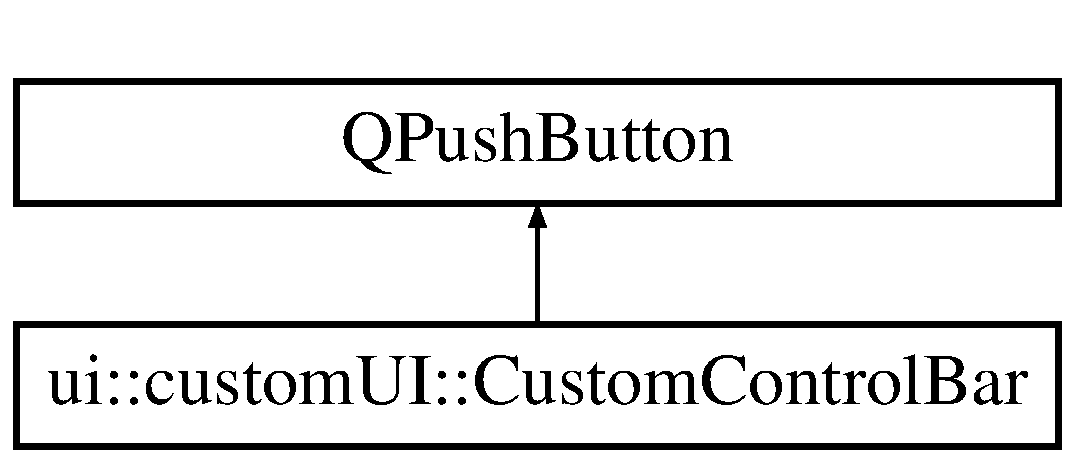
\includegraphics[height=2.000000cm]{classui_1_1custom_u_i_1_1_custom_control_bar}
\end{center}
\end{figure}
\subsection*{Public Member Functions}
\begin{DoxyCompactItemize}
\item 
\mbox{\Hypertarget{classui_1_1custom_u_i_1_1_custom_control_bar_a9329f07f4c566ad4427898976a7c54e9}\label{classui_1_1custom_u_i_1_1_custom_control_bar_a9329f07f4c566ad4427898976a7c54e9}} 
{\bfseries Custom\+Control\+Bar} (Q\+Widget $\ast$parent=nullptr)
\item 
\mbox{\Hypertarget{classui_1_1custom_u_i_1_1_custom_control_bar_a06869826febedb072e3563b67233c1a6}\label{classui_1_1custom_u_i_1_1_custom_control_bar_a06869826febedb072e3563b67233c1a6}} 
void {\bfseries set\+Dark\+Mode} (void)
\item 
\mbox{\Hypertarget{classui_1_1custom_u_i_1_1_custom_control_bar_ad144dfcd0631cf953f6835f725d8fb22}\label{classui_1_1custom_u_i_1_1_custom_control_bar_ad144dfcd0631cf953f6835f725d8fb22}} 
void {\bfseries set\+Light\+Mode} (void)
\item 
\mbox{\Hypertarget{classui_1_1custom_u_i_1_1_custom_control_bar_ad866a00b234d58ea00f485590a939e12}\label{classui_1_1custom_u_i_1_1_custom_control_bar_ad866a00b234d58ea00f485590a939e12}} 
void {\bfseries toggle\+Side} (void)
\item 
\mbox{\Hypertarget{classui_1_1custom_u_i_1_1_custom_control_bar_ab5d80c519c4c0675cc2b1de53a83ba27}\label{classui_1_1custom_u_i_1_1_custom_control_bar_ab5d80c519c4c0675cc2b1de53a83ba27}} 
bool {\bfseries pointing\+Left} (void)
\end{DoxyCompactItemize}
\subsection*{Public Attributes}
\begin{DoxyCompactItemize}
\item 
\mbox{\Hypertarget{classui_1_1custom_u_i_1_1_custom_control_bar_a7d084a4f5eeb2e4f4bdde5b28ab420e5}\label{classui_1_1custom_u_i_1_1_custom_control_bar_a7d084a4f5eeb2e4f4bdde5b28ab420e5}} 
bool {\bfseries dark}
\item 
\mbox{\Hypertarget{classui_1_1custom_u_i_1_1_custom_control_bar_a71286e6b39628683dbbcb8e9d330bf03}\label{classui_1_1custom_u_i_1_1_custom_control_bar_a71286e6b39628683dbbcb8e9d330bf03}} 
bool {\bfseries pointing\+In}
\item 
\mbox{\Hypertarget{classui_1_1custom_u_i_1_1_custom_control_bar_a15b8a21c567bc4ac7ae3ef90dd6091f4}\label{classui_1_1custom_u_i_1_1_custom_control_bar_a15b8a21c567bc4ac7ae3ef90dd6091f4}} 
Q\+Icon $\ast$ {\bfseries dark\+Mode\+Right}
\item 
\mbox{\Hypertarget{classui_1_1custom_u_i_1_1_custom_control_bar_a07e012267522c0d7b6087c5240dcbb4f}\label{classui_1_1custom_u_i_1_1_custom_control_bar_a07e012267522c0d7b6087c5240dcbb4f}} 
Q\+Icon $\ast$ {\bfseries light\+Mode\+Right}
\item 
\mbox{\Hypertarget{classui_1_1custom_u_i_1_1_custom_control_bar_acd10512d13b55401d2642f8f43fc2d17}\label{classui_1_1custom_u_i_1_1_custom_control_bar_acd10512d13b55401d2642f8f43fc2d17}} 
Q\+Icon $\ast$ {\bfseries dark\+Mode\+Left}
\item 
\mbox{\Hypertarget{classui_1_1custom_u_i_1_1_custom_control_bar_a1ebb7a5a1aad7f13191e7d47240f7068}\label{classui_1_1custom_u_i_1_1_custom_control_bar_a1ebb7a5a1aad7f13191e7d47240f7068}} 
Q\+Icon $\ast$ {\bfseries light\+Mode\+Left}
\end{DoxyCompactItemize}


\subsection{Detailed Description}
This class will be removed. 

The documentation for this class was generated from the following files\+:\begin{DoxyCompactItemize}
\item 
ui/custom\+U\+I/customcontrolbar.\+h\item 
ui/custom\+U\+I/customcontrolbar.\+cpp\end{DoxyCompactItemize}

\hypertarget{classui_1_1custom_u_i_1_1_custom_list_widget_item}{}\section{ui\+:\+:custom\+UI\+:\+:Custom\+List\+Widget\+Item Class Reference}
\label{classui_1_1custom_u_i_1_1_custom_list_widget_item}\index{ui\+::custom\+U\+I\+::\+Custom\+List\+Widget\+Item@{ui\+::custom\+U\+I\+::\+Custom\+List\+Widget\+Item}}


This class This class provides a custom impelemntation of a Listwidget.  




{\ttfamily \#include $<$customlistwidgetitem.\+h$>$}

Inheritance diagram for ui\+:\+:custom\+UI\+:\+:Custom\+List\+Widget\+Item\+:\begin{figure}[H]
\begin{center}
\leavevmode
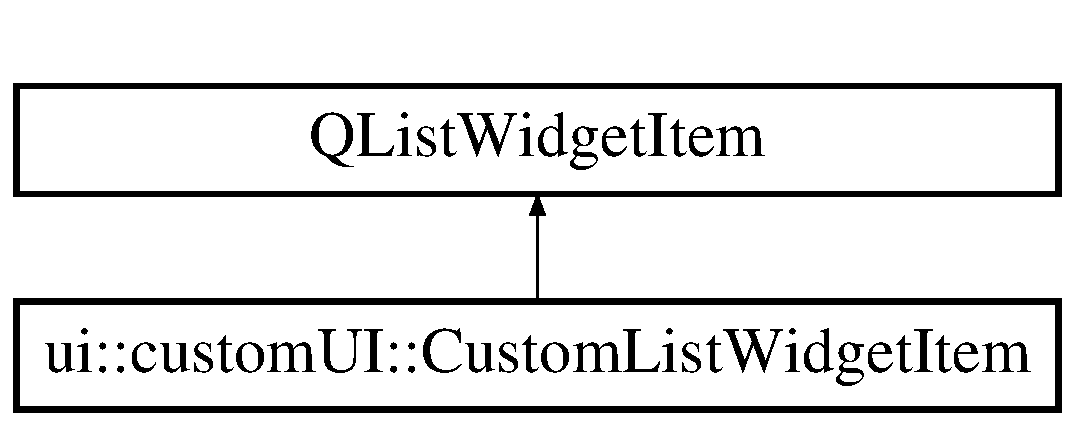
\includegraphics[height=2.000000cm]{classui_1_1custom_u_i_1_1_custom_list_widget_item}
\end{center}
\end{figure}
\subsection*{Public Member Functions}
\begin{DoxyCompactItemize}
\item 
\mbox{\hyperlink{classui_1_1custom_u_i_1_1_custom_list_widget_item_a7da08f342e6eeb0a2a4833c3031a9246}{Custom\+List\+Widget\+Item}} (Q\+String text, Q\+String res=nullptr)
\begin{DoxyCompactList}\small\item\em \mbox{\hyperlink{classui_1_1custom_u_i_1_1_custom_list_widget_item}{Custom\+List\+Widget\+Item}} This constructor creates a new instance of this class. \end{DoxyCompactList}\item 
virtual \mbox{\hyperlink{classui_1_1custom_u_i_1_1_custom_list_widget_item_abe90e419781fb947e684a4dea54568e4}{$\sim$\+Custom\+List\+Widget\+Item}} (void)
\begin{DoxyCompactList}\small\item\em $\sim$\+Custom\+List\+Widget\+Item Destructor \end{DoxyCompactList}\item 
void \mbox{\hyperlink{classui_1_1custom_u_i_1_1_custom_list_widget_item_a71d6b28f6e542c450807f2277ddacdc4}{enable\+Light\+Mode}} (void)
\begin{DoxyCompactList}\small\item\em enable\+Light\+Mode This method enabled the light mode \end{DoxyCompactList}\item 
void \mbox{\hyperlink{classui_1_1custom_u_i_1_1_custom_list_widget_item_a97000c77f8c27f46c8ef2cc0ee824db0}{enable\+Dark\+Mode}} (void)
\begin{DoxyCompactList}\small\item\em enable\+Light\+Mode This method enabled the dark mode \end{DoxyCompactList}\end{DoxyCompactItemize}
\subsection*{Private Attributes}
\begin{DoxyCompactItemize}
\item 
\mbox{\Hypertarget{classui_1_1custom_u_i_1_1_custom_list_widget_item_ac82e362c36815072e8927cd2b5f6011f}\label{classui_1_1custom_u_i_1_1_custom_list_widget_item_ac82e362c36815072e8927cd2b5f6011f}} 
bool \mbox{\hyperlink{classui_1_1custom_u_i_1_1_custom_list_widget_item_ac82e362c36815072e8927cd2b5f6011f}{dark\+\_\+m}}
\begin{DoxyCompactList}\small\item\em dark This attributes detemrines if the darkmode is enabled \end{DoxyCompactList}\item 
\mbox{\Hypertarget{classui_1_1custom_u_i_1_1_custom_list_widget_item_a62ba044883f9b0a2a1abc6e13efb3411}\label{classui_1_1custom_u_i_1_1_custom_list_widget_item_a62ba044883f9b0a2a1abc6e13efb3411}} 
Q\+Icon $\ast$ \mbox{\hyperlink{classui_1_1custom_u_i_1_1_custom_list_widget_item_a62ba044883f9b0a2a1abc6e13efb3411}{dark\+Mode\+Icon\+\_\+m}}
\begin{DoxyCompactList}\small\item\em dark\+Mode This icon contains the image of the darkmode \end{DoxyCompactList}\item 
\mbox{\Hypertarget{classui_1_1custom_u_i_1_1_custom_list_widget_item_a26296177f28c453439f056d550fe9c81}\label{classui_1_1custom_u_i_1_1_custom_list_widget_item_a26296177f28c453439f056d550fe9c81}} 
Q\+Icon $\ast$ \mbox{\hyperlink{classui_1_1custom_u_i_1_1_custom_list_widget_item_a26296177f28c453439f056d550fe9c81}{light\+Mode\+Icon\+\_\+m}}
\begin{DoxyCompactList}\small\item\em dark\+Mode This icon contains the image of the lightmode \end{DoxyCompactList}\end{DoxyCompactItemize}


\subsection{Detailed Description}
This class This class provides a custom impelemntation of a Listwidget. 

This class provides a custom implementation of the Q\+List\+Widget\+Class, it is a wrapper to enable different UI modes, such like dark and light \begin{DoxyAuthor}{Author}
Nils Milewski(10010480) 
\end{DoxyAuthor}


\subsection{Constructor \& Destructor Documentation}
\mbox{\Hypertarget{classui_1_1custom_u_i_1_1_custom_list_widget_item_a7da08f342e6eeb0a2a4833c3031a9246}\label{classui_1_1custom_u_i_1_1_custom_list_widget_item_a7da08f342e6eeb0a2a4833c3031a9246}} 
\index{ui\+::custom\+U\+I\+::\+Custom\+List\+Widget\+Item@{ui\+::custom\+U\+I\+::\+Custom\+List\+Widget\+Item}!Custom\+List\+Widget\+Item@{Custom\+List\+Widget\+Item}}
\index{Custom\+List\+Widget\+Item@{Custom\+List\+Widget\+Item}!ui\+::custom\+U\+I\+::\+Custom\+List\+Widget\+Item@{ui\+::custom\+U\+I\+::\+Custom\+List\+Widget\+Item}}
\subsubsection{\texorpdfstring{Custom\+List\+Widget\+Item()}{CustomListWidgetItem()}}
{\footnotesize\ttfamily Custom\+List\+Widget\+Item\+::\+Custom\+List\+Widget\+Item (\begin{DoxyParamCaption}\item[{Q\+String}]{text,  }\item[{Q\+String}]{res = {\ttfamily nullptr} }\end{DoxyParamCaption})}



\mbox{\hyperlink{classui_1_1custom_u_i_1_1_custom_list_widget_item}{Custom\+List\+Widget\+Item}} This constructor creates a new instance of this class. 

This constructor will initalize all attributes and set the default to darkmode 
\begin{DoxyParams}{Parameters}
{\em text} & Text which the List\+Widget\+Ite should display \\
\hline
{\em res} & Name of the resource, note \+:/images/theme/$<$mode$>$/res/$<$mode$>$/ will be set, use the Icon name, e.\+g. add.\+svg \\
\hline
\end{DoxyParams}
\mbox{\Hypertarget{classui_1_1custom_u_i_1_1_custom_list_widget_item_abe90e419781fb947e684a4dea54568e4}\label{classui_1_1custom_u_i_1_1_custom_list_widget_item_abe90e419781fb947e684a4dea54568e4}} 
\index{ui\+::custom\+U\+I\+::\+Custom\+List\+Widget\+Item@{ui\+::custom\+U\+I\+::\+Custom\+List\+Widget\+Item}!````~Custom\+List\+Widget\+Item@{$\sim$\+Custom\+List\+Widget\+Item}}
\index{````~Custom\+List\+Widget\+Item@{$\sim$\+Custom\+List\+Widget\+Item}!ui\+::custom\+U\+I\+::\+Custom\+List\+Widget\+Item@{ui\+::custom\+U\+I\+::\+Custom\+List\+Widget\+Item}}
\subsubsection{\texorpdfstring{$\sim$\+Custom\+List\+Widget\+Item()}{~CustomListWidgetItem()}}
{\footnotesize\ttfamily Custom\+List\+Widget\+Item\+::$\sim$\+Custom\+List\+Widget\+Item (\begin{DoxyParamCaption}\item[{void}]{ }\end{DoxyParamCaption})\hspace{0.3cm}{\ttfamily [virtual]}}



$\sim$\+Custom\+List\+Widget\+Item Destructor 

This destructor will free up used resources 

\subsection{Member Function Documentation}
\mbox{\Hypertarget{classui_1_1custom_u_i_1_1_custom_list_widget_item_a97000c77f8c27f46c8ef2cc0ee824db0}\label{classui_1_1custom_u_i_1_1_custom_list_widget_item_a97000c77f8c27f46c8ef2cc0ee824db0}} 
\index{ui\+::custom\+U\+I\+::\+Custom\+List\+Widget\+Item@{ui\+::custom\+U\+I\+::\+Custom\+List\+Widget\+Item}!enable\+Dark\+Mode@{enable\+Dark\+Mode}}
\index{enable\+Dark\+Mode@{enable\+Dark\+Mode}!ui\+::custom\+U\+I\+::\+Custom\+List\+Widget\+Item@{ui\+::custom\+U\+I\+::\+Custom\+List\+Widget\+Item}}
\subsubsection{\texorpdfstring{enable\+Dark\+Mode()}{enableDarkMode()}}
{\footnotesize\ttfamily void Custom\+List\+Widget\+Item\+::enable\+Dark\+Mode (\begin{DoxyParamCaption}\item[{void}]{ }\end{DoxyParamCaption})}



enable\+Light\+Mode This method enabled the dark mode 

This method sets the dark\+\_\+m attribute to true and sets the icon to the dark\+Mode\+Icon\+\_\+m \mbox{\Hypertarget{classui_1_1custom_u_i_1_1_custom_list_widget_item_a71d6b28f6e542c450807f2277ddacdc4}\label{classui_1_1custom_u_i_1_1_custom_list_widget_item_a71d6b28f6e542c450807f2277ddacdc4}} 
\index{ui\+::custom\+U\+I\+::\+Custom\+List\+Widget\+Item@{ui\+::custom\+U\+I\+::\+Custom\+List\+Widget\+Item}!enable\+Light\+Mode@{enable\+Light\+Mode}}
\index{enable\+Light\+Mode@{enable\+Light\+Mode}!ui\+::custom\+U\+I\+::\+Custom\+List\+Widget\+Item@{ui\+::custom\+U\+I\+::\+Custom\+List\+Widget\+Item}}
\subsubsection{\texorpdfstring{enable\+Light\+Mode()}{enableLightMode()}}
{\footnotesize\ttfamily void Custom\+List\+Widget\+Item\+::enable\+Light\+Mode (\begin{DoxyParamCaption}\item[{void}]{ }\end{DoxyParamCaption})}



enable\+Light\+Mode This method enabled the light mode 

This method sets the dark\+\_\+m attribute to false and sets the icon to the light\+Mode\+Icon\+\_\+m 

The documentation for this class was generated from the following files\+:\begin{DoxyCompactItemize}
\item 
ui/custom\+U\+I/customlistwidgetitem.\+h\item 
ui/custom\+U\+I/customlistwidgetitem.\+cpp\end{DoxyCompactItemize}

\hypertarget{classui_1_1window_1_1_detail_page}{}\section{ui\+:\+:window\+:\+:Detail\+Page Class Reference}
\label{classui_1_1window_1_1_detail_page}\index{ui\+::window\+::\+Detail\+Page@{ui\+::window\+::\+Detail\+Page}}


This class handles all new created windows.  




{\ttfamily \#include $<$detailpage.\+h$>$}

Inheritance diagram for ui\+:\+:window\+:\+:Detail\+Page\+:\begin{figure}[H]
\begin{center}
\leavevmode
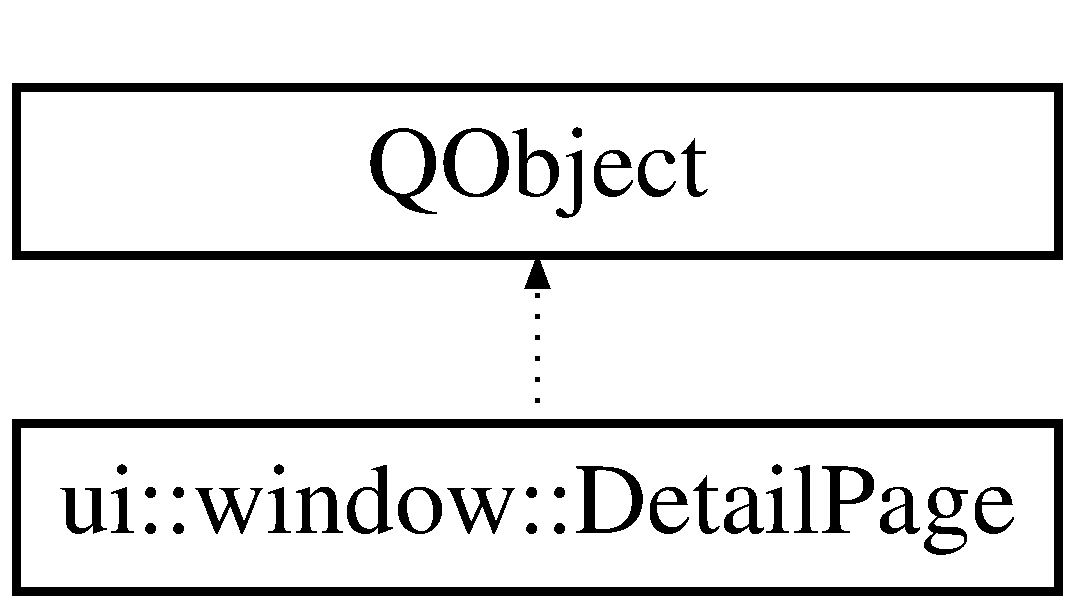
\includegraphics[height=2.000000cm]{classui_1_1window_1_1_detail_page}
\end{center}
\end{figure}
\subsection*{Public Types}
\begin{DoxyCompactItemize}
\item 
\mbox{\Hypertarget{classui_1_1window_1_1_detail_page_a4104cccd964dece9660152be1109e987}\label{classui_1_1window_1_1_detail_page_a4104cccd964dece9660152be1109e987}} 
enum {\bfseries display} \{ {\bfseries Disk\+\_\+\+Info}, 
{\bfseries Partition\+\_\+\+Resize}
 \}
\end{DoxyCompactItemize}
\subsection*{Public Member Functions}
\begin{DoxyCompactItemize}
\item 
\mbox{\hyperlink{classui_1_1window_1_1_detail_page_a151e61733c9f0cfbff77d58f161b15bf}{Detail\+Page}} ()
\begin{DoxyCompactList}\small\item\em \mbox{\hyperlink{classui_1_1window_1_1_detail_page}{Detail\+Page}} Constructor. \end{DoxyCompactList}\item 
virtual \mbox{\hyperlink{classui_1_1window_1_1_detail_page_ab50d547f466fa6b6bba924b79282aae1}{$\sim$\+Detail\+Page}} ()
\begin{DoxyCompactList}\small\item\em $\sim$\+Detail\+Page Destructor \end{DoxyCompactList}\item 
void \mbox{\hyperlink{classui_1_1window_1_1_detail_page_a1bbc24ad94c66e55e29ba208586a5bf5}{toggle\+Page}} (display which)
\begin{DoxyCompactList}\small\item\em toggle\+Page This method toggles the visibility of a window \end{DoxyCompactList}\item 
void \mbox{\hyperlink{classui_1_1window_1_1_detail_page_ad677d96003c9405071abed57a2310c9d}{set\+Disk}} (\mbox{\hyperlink{classcore_1_1disk_1_1_disk}{core\+::disk\+::\+Disk}} $\ast$disk)
\begin{DoxyCompactList}\small\item\em set\+Disk This method sets the workind disk \end{DoxyCompactList}\item 
void \mbox{\hyperlink{classui_1_1window_1_1_detail_page_a2eba9774cf72106a5b87357c2348f5ae}{close}} (void)
\begin{DoxyCompactList}\small\item\em close This method closes all windows \end{DoxyCompactList}\end{DoxyCompactItemize}
\subsection*{Private Attributes}
\begin{DoxyCompactItemize}
\item 
\mbox{\Hypertarget{classui_1_1window_1_1_detail_page_a6e23be528d79660b733da5130b237671}\label{classui_1_1window_1_1_detail_page_a6e23be528d79660b733da5130b237671}} 
\mbox{\hyperlink{classcore_1_1disk_1_1_disk}{core\+::disk\+::\+Disk}} $\ast$ \mbox{\hyperlink{classui_1_1window_1_1_detail_page_a6e23be528d79660b733da5130b237671}{working\+Disk\+\_\+m}}
\begin{DoxyCompactList}\small\item\em working\+Disk\+\_\+m This is the disk which all windows should be using \end{DoxyCompactList}\item 
\mbox{\Hypertarget{classui_1_1window_1_1_detail_page_a8d92bb2023fcec9ea1e5f89b51ca6f5e}\label{classui_1_1window_1_1_detail_page_a8d92bb2023fcec9ea1e5f89b51ca6f5e}} 
\mbox{\hyperlink{classui_1_1window_1_1_disk_info}{Disk\+Info}} $\ast$ \mbox{\hyperlink{classui_1_1window_1_1_detail_page_a8d92bb2023fcec9ea1e5f89b51ca6f5e}{disk\+Info\+Page\+\_\+m}}
\begin{DoxyCompactList}\small\item\em disk\+Info\+Page This page shows all infomration about a specified disk \end{DoxyCompactList}\item 
\mbox{\Hypertarget{classui_1_1window_1_1_detail_page_a03d29770a526ca650e3ed145d800ab1d}\label{classui_1_1window_1_1_detail_page_a03d29770a526ca650e3ed145d800ab1d}} 
\mbox{\hyperlink{classui_1_1window_1_1_resize_partition}{Resize\+Partition}} $\ast$ \mbox{\hyperlink{classui_1_1window_1_1_detail_page_a03d29770a526ca650e3ed145d800ab1d}{resize\+Partition\+\_\+m}}
\begin{DoxyCompactList}\small\item\em disk\+Info\+Page This page allows resizeing a partition from a specific partition of a specified disk \end{DoxyCompactList}\end{DoxyCompactItemize}


\subsection{Detailed Description}
This class handles all new created windows. 

This class is a handler for UI windows, it will create and destroy windows As well as manage their data content. \begin{DoxyAuthor}{Author}
Nils Milewski (10010480) 
\end{DoxyAuthor}


\subsection{Constructor \& Destructor Documentation}
\mbox{\Hypertarget{classui_1_1window_1_1_detail_page_a151e61733c9f0cfbff77d58f161b15bf}\label{classui_1_1window_1_1_detail_page_a151e61733c9f0cfbff77d58f161b15bf}} 
\index{ui\+::window\+::\+Detail\+Page@{ui\+::window\+::\+Detail\+Page}!Detail\+Page@{Detail\+Page}}
\index{Detail\+Page@{Detail\+Page}!ui\+::window\+::\+Detail\+Page@{ui\+::window\+::\+Detail\+Page}}
\subsubsection{\texorpdfstring{Detail\+Page()}{DetailPage()}}
{\footnotesize\ttfamily Detail\+Page\+::\+Detail\+Page (\begin{DoxyParamCaption}{ }\end{DoxyParamCaption})}



\mbox{\hyperlink{classui_1_1window_1_1_detail_page}{Detail\+Page}} Constructor. 

This constructor creates all required attritbutes and windows \mbox{\Hypertarget{classui_1_1window_1_1_detail_page_ab50d547f466fa6b6bba924b79282aae1}\label{classui_1_1window_1_1_detail_page_ab50d547f466fa6b6bba924b79282aae1}} 
\index{ui\+::window\+::\+Detail\+Page@{ui\+::window\+::\+Detail\+Page}!````~Detail\+Page@{$\sim$\+Detail\+Page}}
\index{````~Detail\+Page@{$\sim$\+Detail\+Page}!ui\+::window\+::\+Detail\+Page@{ui\+::window\+::\+Detail\+Page}}
\subsubsection{\texorpdfstring{$\sim$\+Detail\+Page()}{~DetailPage()}}
{\footnotesize\ttfamily Detail\+Page\+::$\sim$\+Detail\+Page (\begin{DoxyParamCaption}{ }\end{DoxyParamCaption})\hspace{0.3cm}{\ttfamily [virtual]}}



$\sim$\+Detail\+Page Destructor 

This destructor calls all windows destructors and frees his used heap memory. It will not destruct the workin\+Disk\+\_\+m attribute. 

\subsection{Member Function Documentation}
\mbox{\Hypertarget{classui_1_1window_1_1_detail_page_a2eba9774cf72106a5b87357c2348f5ae}\label{classui_1_1window_1_1_detail_page_a2eba9774cf72106a5b87357c2348f5ae}} 
\index{ui\+::window\+::\+Detail\+Page@{ui\+::window\+::\+Detail\+Page}!close@{close}}
\index{close@{close}!ui\+::window\+::\+Detail\+Page@{ui\+::window\+::\+Detail\+Page}}
\subsubsection{\texorpdfstring{close()}{close()}}
{\footnotesize\ttfamily void Detail\+Page\+::close (\begin{DoxyParamCaption}\item[{void}]{ }\end{DoxyParamCaption})}



close This method closes all windows 

This method calls the hide method from all available windows \mbox{\Hypertarget{classui_1_1window_1_1_detail_page_ad677d96003c9405071abed57a2310c9d}\label{classui_1_1window_1_1_detail_page_ad677d96003c9405071abed57a2310c9d}} 
\index{ui\+::window\+::\+Detail\+Page@{ui\+::window\+::\+Detail\+Page}!set\+Disk@{set\+Disk}}
\index{set\+Disk@{set\+Disk}!ui\+::window\+::\+Detail\+Page@{ui\+::window\+::\+Detail\+Page}}
\subsubsection{\texorpdfstring{set\+Disk()}{setDisk()}}
{\footnotesize\ttfamily void Detail\+Page\+::set\+Disk (\begin{DoxyParamCaption}\item[{\mbox{\hyperlink{classcore_1_1disk_1_1_disk}{core\+::disk\+::\+Disk}} $\ast$}]{disk }\end{DoxyParamCaption})}



set\+Disk This method sets the workind disk 


\begin{DoxyParams}{Parameters}
{\em disk} & New working disk\\
\hline
\end{DoxyParams}
This method sets the working disk of all windows using their set\+Disk method \mbox{\Hypertarget{classui_1_1window_1_1_detail_page_a1bbc24ad94c66e55e29ba208586a5bf5}\label{classui_1_1window_1_1_detail_page_a1bbc24ad94c66e55e29ba208586a5bf5}} 
\index{ui\+::window\+::\+Detail\+Page@{ui\+::window\+::\+Detail\+Page}!toggle\+Page@{toggle\+Page}}
\index{toggle\+Page@{toggle\+Page}!ui\+::window\+::\+Detail\+Page@{ui\+::window\+::\+Detail\+Page}}
\subsubsection{\texorpdfstring{toggle\+Page()}{togglePage()}}
{\footnotesize\ttfamily void Detail\+Page\+::toggle\+Page (\begin{DoxyParamCaption}\item[{Detail\+Page\+::display}]{which }\end{DoxyParamCaption})}



toggle\+Page This method toggles the visibility of a window 


\begin{DoxyParams}{Parameters}
{\em which} & Which window should be toggled \\
\hline
\end{DoxyParams}
\begin{DoxySeeAlso}{See also}
static enum display
\end{DoxySeeAlso}
This method toggles the visibility of a window. The window must be specified by the parameter which, which is an enum of all possible windows. If a window is allready visible it will hide the window. If a window is allready hidden it will show the window. 

The documentation for this class was generated from the following files\+:\begin{DoxyCompactItemize}
\item 
ui/pages/detailpage.\+h\item 
ui/pages/detailpage.\+cpp\end{DoxyCompactItemize}

\hypertarget{classcore_1_1disk_1_1_disk}{}\section{core\+:\+:disk\+:\+:Disk Class Reference}
\label{classcore_1_1disk_1_1_disk}\index{core\+::disk\+::\+Disk@{core\+::disk\+::\+Disk}}


The \mbox{\hyperlink{classcore_1_1disk_1_1_disk}{Disk}} class.  




{\ttfamily \#include $<$disk.\+h$>$}

\subsection*{Public Member Functions}
\begin{DoxyCompactItemize}
\item 
\mbox{\hyperlink{classcore_1_1disk_1_1_disk_a1531676df8b095dc6e818458aebf9dee}{Disk}} (unsigned long long \mbox{\hyperlink{classcore_1_1disk_1_1_disk_a4f0d7b0ab94fb0ed0a58bb19ce85729f}{capacity}}, std\+::string \mbox{\hyperlink{classcore_1_1disk_1_1_disk_a889c305501805431f1189f179d8281ca}{name}})
\begin{DoxyCompactList}\small\item\em \mbox{\hyperlink{classcore_1_1disk_1_1_disk}{Disk}} Constructor. \end{DoxyCompactList}\item 
\mbox{\hyperlink{classcore_1_1disk_1_1_disk_ad7164897c3af79602e86463065550754}{Disk}} (unsigned long long \mbox{\hyperlink{classcore_1_1disk_1_1_disk_a4f0d7b0ab94fb0ed0a58bb19ce85729f}{capacity}}, const char $\ast$\mbox{\hyperlink{classcore_1_1disk_1_1_disk_a889c305501805431f1189f179d8281ca}{name}})
\begin{DoxyCompactList}\small\item\em \mbox{\hyperlink{classcore_1_1disk_1_1_disk}{Disk}} Constructor. \end{DoxyCompactList}\item 
unsigned long long \mbox{\hyperlink{classcore_1_1disk_1_1_disk_a4f0d7b0ab94fb0ed0a58bb19ce85729f}{capacity}} (void)
\begin{DoxyCompactList}\small\item\em capacity This method returns the disk capacity \end{DoxyCompactList}\item 
const std\+::string \mbox{\hyperlink{classcore_1_1disk_1_1_disk_a889c305501805431f1189f179d8281ca}{name}} (void)
\begin{DoxyCompactList}\small\item\em name This method returns the manufcator name of the disk \end{DoxyCompactList}\item 
\mbox{\hyperlink{classcore_1_1disk_1_1_master_boot_record}{Master\+Boot\+Record}} $\ast$ \mbox{\hyperlink{classcore_1_1disk_1_1_disk_ac3ed02b2b44d2d15039d3616238c0985}{M\+BR}} (void)
\begin{DoxyCompactList}\small\item\em M\+BR This method returns the Master Boot Record. \end{DoxyCompactList}\end{DoxyCompactItemize}
\subsection*{Private Member Functions}
\begin{DoxyCompactItemize}
\item 
\mbox{\hyperlink{classcore_1_1disk_1_1_disk_ad1fec93b14401a2496053fee61ec093e}{Disk}} (\mbox{\hyperlink{classcore_1_1disk_1_1_disk}{Disk}} \&disk)
\begin{DoxyCompactList}\small\item\em \mbox{\hyperlink{classcore_1_1disk_1_1_disk}{Disk}} Copy Constructor. \end{DoxyCompactList}\item 
\mbox{\hyperlink{classcore_1_1disk_1_1_disk_a2c193c2ef0c575fe9ffa77eb2f7cf5ef}{Disk}} (\mbox{\hyperlink{classcore_1_1disk_1_1_disk}{Disk}} $\ast$disk)
\begin{DoxyCompactList}\small\item\em \mbox{\hyperlink{classcore_1_1disk_1_1_disk}{Disk}} Copy Constructor. \end{DoxyCompactList}\end{DoxyCompactItemize}
\subsection*{Private Attributes}
\begin{DoxyCompactItemize}
\item 
\mbox{\Hypertarget{classcore_1_1disk_1_1_disk_a318813d090c1ea19e8cbd71d275906c6}\label{classcore_1_1disk_1_1_disk_a318813d090c1ea19e8cbd71d275906c6}} 
unsigned long long \mbox{\hyperlink{classcore_1_1disk_1_1_disk_a318813d090c1ea19e8cbd71d275906c6}{capacity\+\_\+m}}
\begin{DoxyCompactList}\small\item\em capacity\+\_\+m This attributes contains the size of the disk \end{DoxyCompactList}\item 
\mbox{\Hypertarget{classcore_1_1disk_1_1_disk_a20569196ce0a16f1fe04e8065cb5e233}\label{classcore_1_1disk_1_1_disk_a20569196ce0a16f1fe04e8065cb5e233}} 
\mbox{\hyperlink{classcore_1_1disk_1_1_master_boot_record}{Master\+Boot\+Record}} $\ast$ \mbox{\hyperlink{classcore_1_1disk_1_1_disk_a20569196ce0a16f1fe04e8065cb5e233}{M\+B\+R\+\_\+m}}
\begin{DoxyCompactList}\small\item\em M\+B\+R\+\_\+m This attribute represents a Master Boot Recorc entry. \end{DoxyCompactList}\item 
\mbox{\Hypertarget{classcore_1_1disk_1_1_disk_a9669787c8b3049213956af71a99edf7b}\label{classcore_1_1disk_1_1_disk_a9669787c8b3049213956af71a99edf7b}} 
std\+::string \mbox{\hyperlink{classcore_1_1disk_1_1_disk_a9669787c8b3049213956af71a99edf7b}{name\+\_\+m}}
\begin{DoxyCompactList}\small\item\em name\+\_\+m This attributes contains the manufactor name \end{DoxyCompactList}\end{DoxyCompactItemize}
\subsection*{Friends}
\begin{DoxyCompactItemize}
\item 
\mbox{\Hypertarget{classcore_1_1disk_1_1_disk_ab1a95b006b3b89b708da1cd417d1d96d}\label{classcore_1_1disk_1_1_disk_ab1a95b006b3b89b708da1cd417d1d96d}} 
std\+::ostream \& {\bfseries operator$<$$<$} (std\+::ostream \&os, \mbox{\hyperlink{classcore_1_1disk_1_1_disk}{Disk}} \&disk)
\end{DoxyCompactItemize}


\subsection{Detailed Description}
The \mbox{\hyperlink{classcore_1_1disk_1_1_disk}{Disk}} class. 

This class is a representation of a physical disk \begin{DoxyAuthor}{Author}
Nils Milewski (10010480) 
\end{DoxyAuthor}


\subsection{Constructor \& Destructor Documentation}
\mbox{\Hypertarget{classcore_1_1disk_1_1_disk_ad1fec93b14401a2496053fee61ec093e}\label{classcore_1_1disk_1_1_disk_ad1fec93b14401a2496053fee61ec093e}} 
\index{core\+::disk\+::\+Disk@{core\+::disk\+::\+Disk}!Disk@{Disk}}
\index{Disk@{Disk}!core\+::disk\+::\+Disk@{core\+::disk\+::\+Disk}}
\subsubsection{\texorpdfstring{Disk()}{Disk()}\hspace{0.1cm}{\footnotesize\ttfamily [1/4]}}
{\footnotesize\ttfamily Disk\+::\+Disk (\begin{DoxyParamCaption}\item[{\mbox{\hyperlink{classcore_1_1disk_1_1_disk}{Disk}} \&}]{disk }\end{DoxyParamCaption})\hspace{0.3cm}{\ttfamily [private]}}



\mbox{\hyperlink{classcore_1_1disk_1_1_disk}{Disk}} Copy Constructor. 

A disk copy operation is not allowed as a result to represent a physical hard drive 
\begin{DoxyExceptions}{Exceptions}
{\em Allways} & throws a runtime exception \\
\hline
\end{DoxyExceptions}
\mbox{\Hypertarget{classcore_1_1disk_1_1_disk_a2c193c2ef0c575fe9ffa77eb2f7cf5ef}\label{classcore_1_1disk_1_1_disk_a2c193c2ef0c575fe9ffa77eb2f7cf5ef}} 
\index{core\+::disk\+::\+Disk@{core\+::disk\+::\+Disk}!Disk@{Disk}}
\index{Disk@{Disk}!core\+::disk\+::\+Disk@{core\+::disk\+::\+Disk}}
\subsubsection{\texorpdfstring{Disk()}{Disk()}\hspace{0.1cm}{\footnotesize\ttfamily [2/4]}}
{\footnotesize\ttfamily Disk\+::\+Disk (\begin{DoxyParamCaption}\item[{\mbox{\hyperlink{classcore_1_1disk_1_1_disk}{Disk}} $\ast$}]{disk }\end{DoxyParamCaption})\hspace{0.3cm}{\ttfamily [private]}}



\mbox{\hyperlink{classcore_1_1disk_1_1_disk}{Disk}} Copy Constructor. 

A disk copy operation is not allowed as a result to represent a physical hard drive 
\begin{DoxyExceptions}{Exceptions}
{\em Allways} & throws a runtime exception \\
\hline
\end{DoxyExceptions}
\mbox{\Hypertarget{classcore_1_1disk_1_1_disk_a1531676df8b095dc6e818458aebf9dee}\label{classcore_1_1disk_1_1_disk_a1531676df8b095dc6e818458aebf9dee}} 
\index{core\+::disk\+::\+Disk@{core\+::disk\+::\+Disk}!Disk@{Disk}}
\index{Disk@{Disk}!core\+::disk\+::\+Disk@{core\+::disk\+::\+Disk}}
\subsubsection{\texorpdfstring{Disk()}{Disk()}\hspace{0.1cm}{\footnotesize\ttfamily [3/4]}}
{\footnotesize\ttfamily Disk\+::\+Disk (\begin{DoxyParamCaption}\item[{unsigned long long}]{capacity,  }\item[{std\+::string}]{name }\end{DoxyParamCaption})}



\mbox{\hyperlink{classcore_1_1disk_1_1_disk}{Disk}} Constructor. 

This constructor creates a new \mbox{\hyperlink{classcore_1_1disk_1_1_disk}{Disk}} with an empty Master Boot Record 
\begin{DoxyParams}{Parameters}
{\em capacity} & This argument will be assigned to capacity\+\_\+m and specify the disk capactiy \\
\hline
{\em name} & This argument will be assigned to name\+\_\+m and specify the manufcator name \\
\hline
\end{DoxyParams}
\mbox{\Hypertarget{classcore_1_1disk_1_1_disk_ad7164897c3af79602e86463065550754}\label{classcore_1_1disk_1_1_disk_ad7164897c3af79602e86463065550754}} 
\index{core\+::disk\+::\+Disk@{core\+::disk\+::\+Disk}!Disk@{Disk}}
\index{Disk@{Disk}!core\+::disk\+::\+Disk@{core\+::disk\+::\+Disk}}
\subsubsection{\texorpdfstring{Disk()}{Disk()}\hspace{0.1cm}{\footnotesize\ttfamily [4/4]}}
{\footnotesize\ttfamily Disk\+::\+Disk (\begin{DoxyParamCaption}\item[{unsigned long long}]{capacity,  }\item[{const char $\ast$}]{name }\end{DoxyParamCaption})}



\mbox{\hyperlink{classcore_1_1disk_1_1_disk}{Disk}} Constructor. 

This constructor creates a new \mbox{\hyperlink{classcore_1_1disk_1_1_disk}{Disk}} with an empty Master Boot Record 
\begin{DoxyParams}{Parameters}
{\em capacity} & This argument will be assigned to capacity\+\_\+m and specify the disk capactiy \\
\hline
{\em name} & This argument will be assigned to name\+\_\+m and specify the manufcator name \\
\hline
\end{DoxyParams}


\subsection{Member Function Documentation}
\mbox{\Hypertarget{classcore_1_1disk_1_1_disk_a4f0d7b0ab94fb0ed0a58bb19ce85729f}\label{classcore_1_1disk_1_1_disk_a4f0d7b0ab94fb0ed0a58bb19ce85729f}} 
\index{core\+::disk\+::\+Disk@{core\+::disk\+::\+Disk}!capacity@{capacity}}
\index{capacity@{capacity}!core\+::disk\+::\+Disk@{core\+::disk\+::\+Disk}}
\subsubsection{\texorpdfstring{capacity()}{capacity()}}
{\footnotesize\ttfamily unsigned long long Disk\+::capacity (\begin{DoxyParamCaption}\item[{void}]{ }\end{DoxyParamCaption})}



capacity This method returns the disk capacity 

\begin{DoxyReturn}{Returns}
capacity\+\_\+m 
\end{DoxyReturn}
\mbox{\Hypertarget{classcore_1_1disk_1_1_disk_ac3ed02b2b44d2d15039d3616238c0985}\label{classcore_1_1disk_1_1_disk_ac3ed02b2b44d2d15039d3616238c0985}} 
\index{core\+::disk\+::\+Disk@{core\+::disk\+::\+Disk}!M\+BR@{M\+BR}}
\index{M\+BR@{M\+BR}!core\+::disk\+::\+Disk@{core\+::disk\+::\+Disk}}
\subsubsection{\texorpdfstring{M\+B\+R()}{MBR()}}
{\footnotesize\ttfamily \mbox{\hyperlink{classcore_1_1disk_1_1_master_boot_record}{Master\+Boot\+Record}} $\ast$ Disk\+::\+M\+BR (\begin{DoxyParamCaption}\item[{void}]{ }\end{DoxyParamCaption})}



M\+BR This method returns the Master Boot Record. 

\begin{DoxyReturn}{Returns}
mbr\+\_\+m 
\end{DoxyReturn}
\mbox{\Hypertarget{classcore_1_1disk_1_1_disk_a889c305501805431f1189f179d8281ca}\label{classcore_1_1disk_1_1_disk_a889c305501805431f1189f179d8281ca}} 
\index{core\+::disk\+::\+Disk@{core\+::disk\+::\+Disk}!name@{name}}
\index{name@{name}!core\+::disk\+::\+Disk@{core\+::disk\+::\+Disk}}
\subsubsection{\texorpdfstring{name()}{name()}}
{\footnotesize\ttfamily const std\+::string Disk\+::name (\begin{DoxyParamCaption}\item[{void}]{ }\end{DoxyParamCaption})}



name This method returns the manufcator name of the disk 

\begin{DoxyReturn}{Returns}
name\+\_\+m 
\end{DoxyReturn}


The documentation for this class was generated from the following files\+:\begin{DoxyCompactItemize}
\item 
core/disk.\+h\item 
core/disk.\+cpp\end{DoxyCompactItemize}

\hypertarget{classui_1_1window_1_1_disk_info}{}\section{ui\+:\+:window\+:\+:Disk\+Info Class Reference}
\label{classui_1_1window_1_1_disk_info}\index{ui\+::window\+::\+Disk\+Info@{ui\+::window\+::\+Disk\+Info}}


This class provides a disk info window.  




{\ttfamily \#include $<$diskinfo.\+h$>$}

Inheritance diagram for ui\+:\+:window\+:\+:Disk\+Info\+:\begin{figure}[H]
\begin{center}
\leavevmode
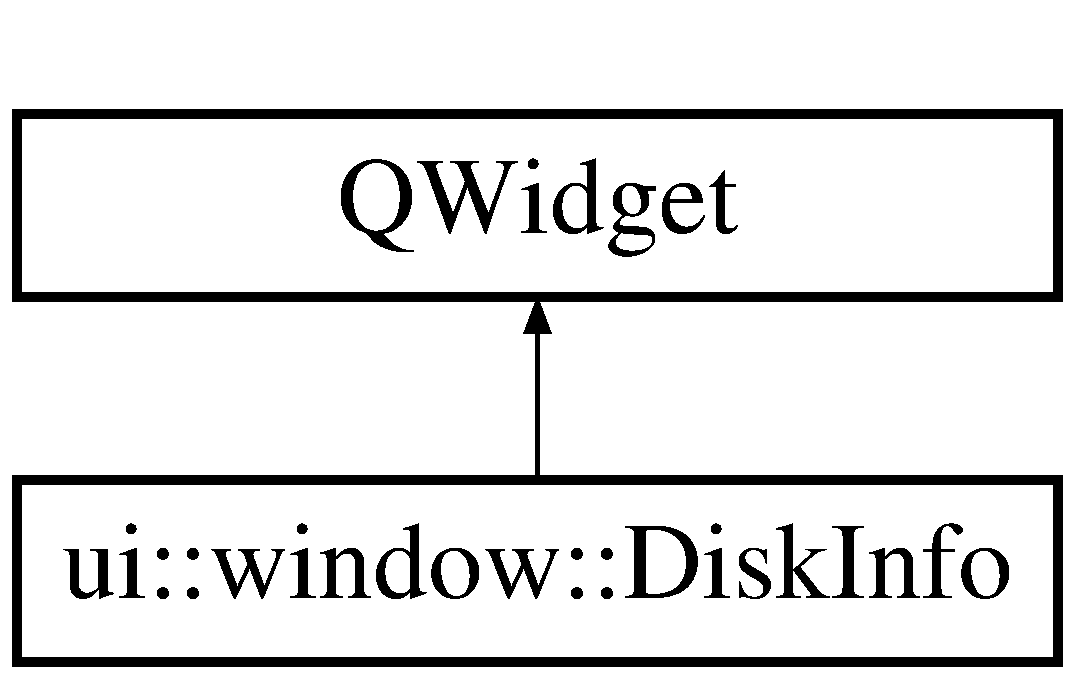
\includegraphics[height=2.000000cm]{classui_1_1window_1_1_disk_info}
\end{center}
\end{figure}
\subsection*{Public Member Functions}
\begin{DoxyCompactItemize}
\item 
\mbox{\hyperlink{classui_1_1window_1_1_disk_info_aca4cde2e854e44f42f3edb8c9bba47ea}{Disk\+Info}} ()
\begin{DoxyCompactList}\small\item\em \mbox{\hyperlink{classui_1_1window_1_1_disk_info}{Disk\+Info}} Constructor. \end{DoxyCompactList}\item 
\mbox{\hyperlink{classui_1_1window_1_1_disk_info_a8a4c3385e2661ba6dc614d00f8dec9d9}{$\sim$\+Disk\+Info}} ()
\begin{DoxyCompactList}\small\item\em $\sim$\+Disk\+Info Destructor \end{DoxyCompactList}\item 
void \mbox{\hyperlink{classui_1_1window_1_1_disk_info_ad818d3e209f7458d33d79a354958035b}{set\+Disk}} (\mbox{\hyperlink{classcore_1_1disk_1_1_disk}{core\+::disk\+::\+Disk}} $\ast$\mbox{\hyperlink{classui_1_1window_1_1_disk_info_a61fcd8caba70cb0c493618e7263a0015}{working\+Disk\+\_\+m}})
\begin{DoxyCompactList}\small\item\em set\+Disk This method sets the working disk \end{DoxyCompactList}\end{DoxyCompactItemize}
\subsection*{Private Attributes}
\begin{DoxyCompactItemize}
\item 
\mbox{\Hypertarget{classui_1_1window_1_1_disk_info_aeafc105508e39cb65fa96cfab0952767}\label{classui_1_1window_1_1_disk_info_aeafc105508e39cb65fa96cfab0952767}} 
Q\+Grid\+Layout $\ast$ \mbox{\hyperlink{classui_1_1window_1_1_disk_info_aeafc105508e39cb65fa96cfab0952767}{disk\+Layout}}
\begin{DoxyCompactList}\small\item\em disk\+Layout This provides a container for the disk info layout \end{DoxyCompactList}\item 
\mbox{\Hypertarget{classui_1_1window_1_1_disk_info_a4f88b60bcb68c4501190811842c24ccf}\label{classui_1_1window_1_1_disk_info_a4f88b60bcb68c4501190811842c24ccf}} 
Q\+Grid\+Layout $\ast$ \mbox{\hyperlink{classui_1_1window_1_1_disk_info_a4f88b60bcb68c4501190811842c24ccf}{partition1\+Layout}}
\begin{DoxyCompactList}\small\item\em partition1\+Layout This provides a container for the parititon 1 \end{DoxyCompactList}\item 
\mbox{\Hypertarget{classui_1_1window_1_1_disk_info_aa51f73e26e08b76b31db591c52b2f533}\label{classui_1_1window_1_1_disk_info_aa51f73e26e08b76b31db591c52b2f533}} 
Q\+Grid\+Layout $\ast$ \mbox{\hyperlink{classui_1_1window_1_1_disk_info_aa51f73e26e08b76b31db591c52b2f533}{partition2\+Layout}}
\begin{DoxyCompactList}\small\item\em partition1\+Layout This provides a container for the parititon 2 \end{DoxyCompactList}\item 
\mbox{\Hypertarget{classui_1_1window_1_1_disk_info_a8d335504811b65dcc19a1f6014508857}\label{classui_1_1window_1_1_disk_info_a8d335504811b65dcc19a1f6014508857}} 
Q\+Grid\+Layout $\ast$ \mbox{\hyperlink{classui_1_1window_1_1_disk_info_a8d335504811b65dcc19a1f6014508857}{partition3\+Layout}}
\begin{DoxyCompactList}\small\item\em partition1\+Layout This provides a container for the parititon 3 \end{DoxyCompactList}\item 
\mbox{\Hypertarget{classui_1_1window_1_1_disk_info_a7bf34bab44808bc3a025d7ff04f1131c}\label{classui_1_1window_1_1_disk_info_a7bf34bab44808bc3a025d7ff04f1131c}} 
Q\+Grid\+Layout $\ast$ \mbox{\hyperlink{classui_1_1window_1_1_disk_info_a7bf34bab44808bc3a025d7ff04f1131c}{partition4\+Layout}}
\begin{DoxyCompactList}\small\item\em partition1\+Layout This provides a container for the parititon 4 \end{DoxyCompactList}\item 
\mbox{\Hypertarget{classui_1_1window_1_1_disk_info_af49e29a7007689ae42eb22e9e7d44d85}\label{classui_1_1window_1_1_disk_info_af49e29a7007689ae42eb22e9e7d44d85}} 
Q\+Label $\ast$ \mbox{\hyperlink{classui_1_1window_1_1_disk_info_af49e29a7007689ae42eb22e9e7d44d85}{lb\+Disk\+Capacity}}
\begin{DoxyCompactList}\small\item\em lb\+Disk\+Capacity This UI element provides the displaying of the space functionality \end{DoxyCompactList}\item 
\mbox{\Hypertarget{classui_1_1window_1_1_disk_info_a3512c625ec97e79a49976abc310ff812}\label{classui_1_1window_1_1_disk_info_a3512c625ec97e79a49976abc310ff812}} 
Q\+Label $\ast$ \mbox{\hyperlink{classui_1_1window_1_1_disk_info_a3512c625ec97e79a49976abc310ff812}{lb\+Disk\+Name}}
\begin{DoxyCompactList}\small\item\em lb\+Disk\+Name This UI element provides the displaying of the disk name \end{DoxyCompactList}\item 
\mbox{\Hypertarget{classui_1_1window_1_1_disk_info_a67caeff64a4088f077001a83b4d24545}\label{classui_1_1window_1_1_disk_info_a67caeff64a4088f077001a83b4d24545}} 
Q\+Label $\ast$ \mbox{\hyperlink{classui_1_1window_1_1_disk_info_a67caeff64a4088f077001a83b4d24545}{lb\+Partition1\+Size}}
\begin{DoxyCompactList}\small\item\em lb\+Partition1\+Size This UI element provides the display of partition 1 size \end{DoxyCompactList}\item 
\mbox{\Hypertarget{classui_1_1window_1_1_disk_info_ab4b828f288920d306d5e5502acd6234e}\label{classui_1_1window_1_1_disk_info_ab4b828f288920d306d5e5502acd6234e}} 
Q\+Label $\ast$ \mbox{\hyperlink{classui_1_1window_1_1_disk_info_ab4b828f288920d306d5e5502acd6234e}{lb\+Partition1\+Amount\+Blocks}}
\begin{DoxyCompactList}\small\item\em lb\+Partition1\+Amount\+Blocks This UI element provides the display of partition 1 used blocks \end{DoxyCompactList}\item 
\mbox{\Hypertarget{classui_1_1window_1_1_disk_info_a15ba61260c684e95dd97fa92674a927e}\label{classui_1_1window_1_1_disk_info_a15ba61260c684e95dd97fa92674a927e}} 
Q\+Label $\ast$ \mbox{\hyperlink{classui_1_1window_1_1_disk_info_a15ba61260c684e95dd97fa92674a927e}{lb\+Partition1\+Mounted}}
\begin{DoxyCompactList}\small\item\em lb\+Partition1\+Mounted This UI element provides the display about the mounted state of partition 1 \end{DoxyCompactList}\item 
\mbox{\Hypertarget{classui_1_1window_1_1_disk_info_aa81ccf5936d3c5a683b429299901a623}\label{classui_1_1window_1_1_disk_info_aa81ccf5936d3c5a683b429299901a623}} 
Q\+Label $\ast$ \mbox{\hyperlink{classui_1_1window_1_1_disk_info_aa81ccf5936d3c5a683b429299901a623}{lb\+Partition2\+Size}}
\begin{DoxyCompactList}\small\item\em lb\+Partition1\+Size This UI element provides the display of partition 2 size \end{DoxyCompactList}\item 
\mbox{\Hypertarget{classui_1_1window_1_1_disk_info_a40396213defabc8a9b91bda033c2b85e}\label{classui_1_1window_1_1_disk_info_a40396213defabc8a9b91bda033c2b85e}} 
Q\+Label $\ast$ \mbox{\hyperlink{classui_1_1window_1_1_disk_info_a40396213defabc8a9b91bda033c2b85e}{lb\+Partition2\+Amount\+Blocks}}
\begin{DoxyCompactList}\small\item\em lb\+Partition1\+Amount\+Blocks This UI element provides the display of partition 2 used blocks \end{DoxyCompactList}\item 
\mbox{\Hypertarget{classui_1_1window_1_1_disk_info_aeba5bada8031f9ed4e73f8411dd78591}\label{classui_1_1window_1_1_disk_info_aeba5bada8031f9ed4e73f8411dd78591}} 
Q\+Label $\ast$ \mbox{\hyperlink{classui_1_1window_1_1_disk_info_aeba5bada8031f9ed4e73f8411dd78591}{lb\+Partition2\+Mounted}}
\begin{DoxyCompactList}\small\item\em lb\+Partition1\+Mounted This UI element provides the display about the mounted state of partition 2 \end{DoxyCompactList}\item 
\mbox{\Hypertarget{classui_1_1window_1_1_disk_info_a97603510a38aaf5d13c550aa606f4c99}\label{classui_1_1window_1_1_disk_info_a97603510a38aaf5d13c550aa606f4c99}} 
Q\+Label $\ast$ \mbox{\hyperlink{classui_1_1window_1_1_disk_info_a97603510a38aaf5d13c550aa606f4c99}{lb\+Partition3\+Size}}
\begin{DoxyCompactList}\small\item\em lb\+Partition1\+Size This UI element provides the display of partition 3 size \end{DoxyCompactList}\item 
\mbox{\Hypertarget{classui_1_1window_1_1_disk_info_a05b4a04aee897e5a589b892d5462e756}\label{classui_1_1window_1_1_disk_info_a05b4a04aee897e5a589b892d5462e756}} 
Q\+Label $\ast$ \mbox{\hyperlink{classui_1_1window_1_1_disk_info_a05b4a04aee897e5a589b892d5462e756}{lb\+Partition3\+Amount\+Blocks}}
\begin{DoxyCompactList}\small\item\em lb\+Partition1\+Amount\+Blocks This UI element provides the display of partition 3 used blocks \end{DoxyCompactList}\item 
\mbox{\Hypertarget{classui_1_1window_1_1_disk_info_ae03aff76e9ca7625a5b6dd96f6d3f478}\label{classui_1_1window_1_1_disk_info_ae03aff76e9ca7625a5b6dd96f6d3f478}} 
Q\+Label $\ast$ \mbox{\hyperlink{classui_1_1window_1_1_disk_info_ae03aff76e9ca7625a5b6dd96f6d3f478}{lb\+Partition3\+Mounted}}
\begin{DoxyCompactList}\small\item\em lb\+Partition1\+Mounted This UI element provides the display about the mounted state of partition 3 \end{DoxyCompactList}\item 
\mbox{\Hypertarget{classui_1_1window_1_1_disk_info_afd7d0629887029eb93a2842192eaff35}\label{classui_1_1window_1_1_disk_info_afd7d0629887029eb93a2842192eaff35}} 
Q\+Label $\ast$ \mbox{\hyperlink{classui_1_1window_1_1_disk_info_afd7d0629887029eb93a2842192eaff35}{lb\+Partition4\+Size}}
\begin{DoxyCompactList}\small\item\em lb\+Partition1\+Size This UI element provides the display of partition 4 size \end{DoxyCompactList}\item 
\mbox{\Hypertarget{classui_1_1window_1_1_disk_info_a5cc2f462a187529316a3203eebd3492a}\label{classui_1_1window_1_1_disk_info_a5cc2f462a187529316a3203eebd3492a}} 
Q\+Label $\ast$ \mbox{\hyperlink{classui_1_1window_1_1_disk_info_a5cc2f462a187529316a3203eebd3492a}{lb\+Partition4\+Amount\+Blocks}}
\begin{DoxyCompactList}\small\item\em lb\+Partition1\+Amount\+Blocks This UI element provides the display of partition 4 used blocks \end{DoxyCompactList}\item 
\mbox{\Hypertarget{classui_1_1window_1_1_disk_info_a4bf4decf4fd58a568d31cffd3fbcd9f3}\label{classui_1_1window_1_1_disk_info_a4bf4decf4fd58a568d31cffd3fbcd9f3}} 
Q\+Label $\ast$ \mbox{\hyperlink{classui_1_1window_1_1_disk_info_a4bf4decf4fd58a568d31cffd3fbcd9f3}{lb\+Partition4\+Mounted}}
\begin{DoxyCompactList}\small\item\em lb\+Partition1\+Mounted This UI element provides the display about the mounted state of partition 4 \end{DoxyCompactList}\item 
\mbox{\Hypertarget{classui_1_1window_1_1_disk_info_a61fcd8caba70cb0c493618e7263a0015}\label{classui_1_1window_1_1_disk_info_a61fcd8caba70cb0c493618e7263a0015}} 
\mbox{\hyperlink{classcore_1_1disk_1_1_disk}{core\+::disk\+::\+Disk}} $\ast$ \mbox{\hyperlink{classui_1_1window_1_1_disk_info_a61fcd8caba70cb0c493618e7263a0015}{working\+Disk\+\_\+m}}
\begin{DoxyCompactList}\small\item\em working\+Disk\+\_\+m This attribute is used as the disk which all information contains \end{DoxyCompactList}\end{DoxyCompactItemize}


\subsection{Detailed Description}
This class provides a disk info window. 

This class is a window which displays all basic information about a disk As basic information we understand the name, size and M\+BR Entries. From the M\+BR entry only the partitions are shown with the basic information \begin{DoxyAuthor}{Author}
Nils Milewski (10010480) 
\end{DoxyAuthor}


\subsection{Constructor \& Destructor Documentation}
\mbox{\Hypertarget{classui_1_1window_1_1_disk_info_aca4cde2e854e44f42f3edb8c9bba47ea}\label{classui_1_1window_1_1_disk_info_aca4cde2e854e44f42f3edb8c9bba47ea}} 
\index{ui\+::window\+::\+Disk\+Info@{ui\+::window\+::\+Disk\+Info}!Disk\+Info@{Disk\+Info}}
\index{Disk\+Info@{Disk\+Info}!ui\+::window\+::\+Disk\+Info@{ui\+::window\+::\+Disk\+Info}}
\subsubsection{\texorpdfstring{Disk\+Info()}{DiskInfo()}}
{\footnotesize\ttfamily Disk\+Info\+::\+Disk\+Info (\begin{DoxyParamCaption}{ }\end{DoxyParamCaption})}



\mbox{\hyperlink{classui_1_1window_1_1_disk_info}{Disk\+Info}} Constructor. 

This constructor initalizes all required attributes and UI Elements, it will also create the whole UI. \mbox{\Hypertarget{classui_1_1window_1_1_disk_info_a8a4c3385e2661ba6dc614d00f8dec9d9}\label{classui_1_1window_1_1_disk_info_a8a4c3385e2661ba6dc614d00f8dec9d9}} 
\index{ui\+::window\+::\+Disk\+Info@{ui\+::window\+::\+Disk\+Info}!````~Disk\+Info@{$\sim$\+Disk\+Info}}
\index{````~Disk\+Info@{$\sim$\+Disk\+Info}!ui\+::window\+::\+Disk\+Info@{ui\+::window\+::\+Disk\+Info}}
\subsubsection{\texorpdfstring{$\sim$\+Disk\+Info()}{~DiskInfo()}}
{\footnotesize\ttfamily Disk\+Info\+::$\sim$\+Disk\+Info (\begin{DoxyParamCaption}{ }\end{DoxyParamCaption})}



$\sim$\+Disk\+Info Destructor 

This destructor will destroy all UI elements. It will not destruct the working\+Disk\+\_\+m attirbute 

\subsection{Member Function Documentation}
\mbox{\Hypertarget{classui_1_1window_1_1_disk_info_ad818d3e209f7458d33d79a354958035b}\label{classui_1_1window_1_1_disk_info_ad818d3e209f7458d33d79a354958035b}} 
\index{ui\+::window\+::\+Disk\+Info@{ui\+::window\+::\+Disk\+Info}!set\+Disk@{set\+Disk}}
\index{set\+Disk@{set\+Disk}!ui\+::window\+::\+Disk\+Info@{ui\+::window\+::\+Disk\+Info}}
\subsubsection{\texorpdfstring{set\+Disk()}{setDisk()}}
{\footnotesize\ttfamily void Disk\+Info\+::set\+Disk (\begin{DoxyParamCaption}\item[{\mbox{\hyperlink{classcore_1_1disk_1_1_disk}{core\+::disk\+::\+Disk}} $\ast$}]{working\+Disk\+\_\+m }\end{DoxyParamCaption})}



set\+Disk This method sets the working disk 


\begin{DoxyParams}{Parameters}
{\em disk} & New working disk\\
\hline
\end{DoxyParams}
This method sets the working disk of this windows 

The documentation for this class was generated from the following files\+:\begin{DoxyCompactItemize}
\item 
ui/pages/diskinfo.\+h\item 
ui/pages/diskinfo.\+cpp\end{DoxyCompactItemize}

\hypertarget{classui_1_1wizard_1_1pages_1_1_disk_page}{}\section{ui\+:\+:wizard\+:\+:pages\+:\+:Disk\+Page Class Reference}
\label{classui_1_1wizard_1_1pages_1_1_disk_page}\index{ui\+::wizard\+::pages\+::\+Disk\+Page@{ui\+::wizard\+::pages\+::\+Disk\+Page}}


This class provides a custom implementation of a wizard page.  




{\ttfamily \#include $<$diskpage.\+h$>$}

Inheritance diagram for ui\+:\+:wizard\+:\+:pages\+:\+:Disk\+Page\+:\begin{figure}[H]
\begin{center}
\leavevmode
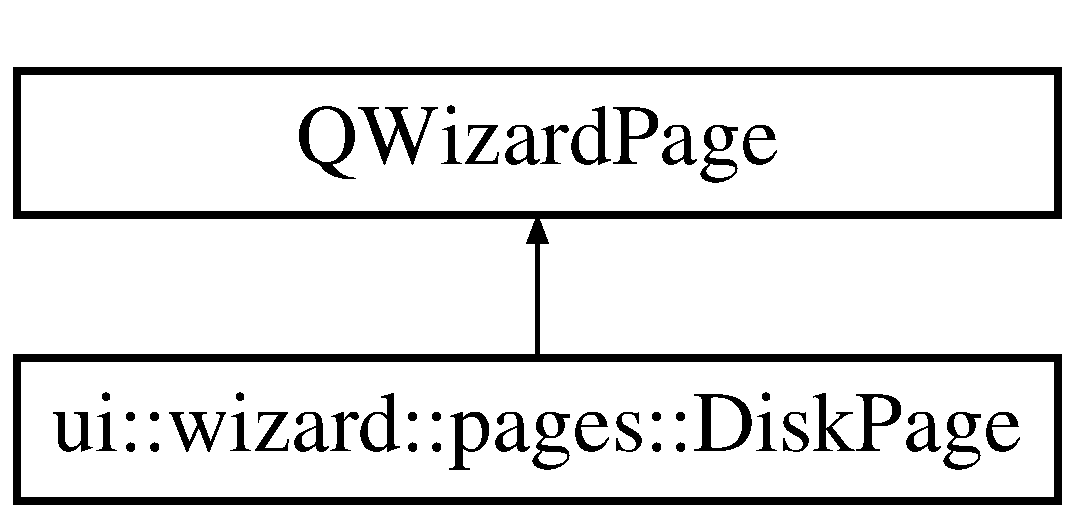
\includegraphics[height=2.000000cm]{classui_1_1wizard_1_1pages_1_1_disk_page}
\end{center}
\end{figure}
\subsection*{Public Member Functions}
\begin{DoxyCompactItemize}
\item 
\mbox{\hyperlink{classui_1_1wizard_1_1pages_1_1_disk_page_a7962a9459e0cb49c1f587de2d595cc04}{Disk\+Page}} (Q\+Widget $\ast$parent=nullptr)
\begin{DoxyCompactList}\small\item\em \mbox{\hyperlink{classui_1_1wizard_1_1pages_1_1_disk_page}{Disk\+Page}} This is a constructor. \end{DoxyCompactList}\item 
virtual \mbox{\hyperlink{classui_1_1wizard_1_1pages_1_1_disk_page_adb9feba7b9ac2bbfa5b944920a2328e3}{$\sim$\+Disk\+Page}} (void) override
\begin{DoxyCompactList}\small\item\em $\sim$\+Disk\+Page Destructor \end{DoxyCompactList}\item 
int \mbox{\hyperlink{classui_1_1wizard_1_1pages_1_1_disk_page_ac6cb9ab53d89deac235d43251b333354}{next\+Id}} () const override
\begin{DoxyCompactList}\small\item\em next\+Id This method returns the next id \end{DoxyCompactList}\end{DoxyCompactItemize}


\subsection{Detailed Description}
This class provides a custom implementation of a wizard page. 

This class is a custom implementation of a wizard page It request all required information for a disk creation \begin{DoxyAuthor}{Author}
Nils Milewski (10010480) 
\end{DoxyAuthor}


\subsection{Constructor \& Destructor Documentation}
\mbox{\Hypertarget{classui_1_1wizard_1_1pages_1_1_disk_page_a7962a9459e0cb49c1f587de2d595cc04}\label{classui_1_1wizard_1_1pages_1_1_disk_page_a7962a9459e0cb49c1f587de2d595cc04}} 
\index{ui\+::wizard\+::pages\+::\+Disk\+Page@{ui\+::wizard\+::pages\+::\+Disk\+Page}!Disk\+Page@{Disk\+Page}}
\index{Disk\+Page@{Disk\+Page}!ui\+::wizard\+::pages\+::\+Disk\+Page@{ui\+::wizard\+::pages\+::\+Disk\+Page}}
\subsubsection{\texorpdfstring{Disk\+Page()}{DiskPage()}}
{\footnotesize\ttfamily Disk\+Page\+::\+Disk\+Page (\begin{DoxyParamCaption}\item[{Q\+Widget $\ast$}]{parent = {\ttfamily nullptr} }\end{DoxyParamCaption})}



\mbox{\hyperlink{classui_1_1wizard_1_1pages_1_1_disk_page}{Disk\+Page}} This is a constructor. 

This constructor creates the layout of the page and set required attributes 
\begin{DoxyParams}{Parameters}
{\em parent} & Parent object which this object is associated with \\
\hline
\end{DoxyParams}
\mbox{\Hypertarget{classui_1_1wizard_1_1pages_1_1_disk_page_adb9feba7b9ac2bbfa5b944920a2328e3}\label{classui_1_1wizard_1_1pages_1_1_disk_page_adb9feba7b9ac2bbfa5b944920a2328e3}} 
\index{ui\+::wizard\+::pages\+::\+Disk\+Page@{ui\+::wizard\+::pages\+::\+Disk\+Page}!````~Disk\+Page@{$\sim$\+Disk\+Page}}
\index{````~Disk\+Page@{$\sim$\+Disk\+Page}!ui\+::wizard\+::pages\+::\+Disk\+Page@{ui\+::wizard\+::pages\+::\+Disk\+Page}}
\subsubsection{\texorpdfstring{$\sim$\+Disk\+Page()}{~DiskPage()}}
{\footnotesize\ttfamily Disk\+Page\+::$\sim$\+Disk\+Page (\begin{DoxyParamCaption}\item[{void}]{ }\end{DoxyParamCaption})\hspace{0.3cm}{\ttfamily [override]}, {\ttfamily [virtual]}}



$\sim$\+Disk\+Page Destructor 

This destructor will free up used resources 

\subsection{Member Function Documentation}
\mbox{\Hypertarget{classui_1_1wizard_1_1pages_1_1_disk_page_ac6cb9ab53d89deac235d43251b333354}\label{classui_1_1wizard_1_1pages_1_1_disk_page_ac6cb9ab53d89deac235d43251b333354}} 
\index{ui\+::wizard\+::pages\+::\+Disk\+Page@{ui\+::wizard\+::pages\+::\+Disk\+Page}!next\+Id@{next\+Id}}
\index{next\+Id@{next\+Id}!ui\+::wizard\+::pages\+::\+Disk\+Page@{ui\+::wizard\+::pages\+::\+Disk\+Page}}
\subsubsection{\texorpdfstring{next\+Id()}{nextId()}}
{\footnotesize\ttfamily int Disk\+Page\+::next\+Id (\begin{DoxyParamCaption}{ }\end{DoxyParamCaption}) const\hspace{0.3cm}{\ttfamily [override]}}



next\+Id This method returns the next id 

This method overrides the default implementation to utilize different intro pages. It will return the enum of next\+\_\+page to differenciate between disk and partition pages \begin{DoxyReturn}{Returns}
Next id for the wizard 
\end{DoxyReturn}


The documentation for this class was generated from the following files\+:\begin{DoxyCompactItemize}
\item 
ui/wizard/pages/diskpage.\+h\item 
ui/wizard/pages/diskpage.\+cpp\end{DoxyCompactItemize}

\hypertarget{classui_1_1wizard_1_1_disk_wizard}{}\section{ui\+:\+:wizard\+:\+:Disk\+Wizard Class Reference}
\label{classui_1_1wizard_1_1_disk_wizard}\index{ui\+::wizard\+::\+Disk\+Wizard@{ui\+::wizard\+::\+Disk\+Wizard}}


This class this class implements a wizard.  




{\ttfamily \#include $<$diskwizard.\+h$>$}

Inheritance diagram for ui\+:\+:wizard\+:\+:Disk\+Wizard\+:\begin{figure}[H]
\begin{center}
\leavevmode
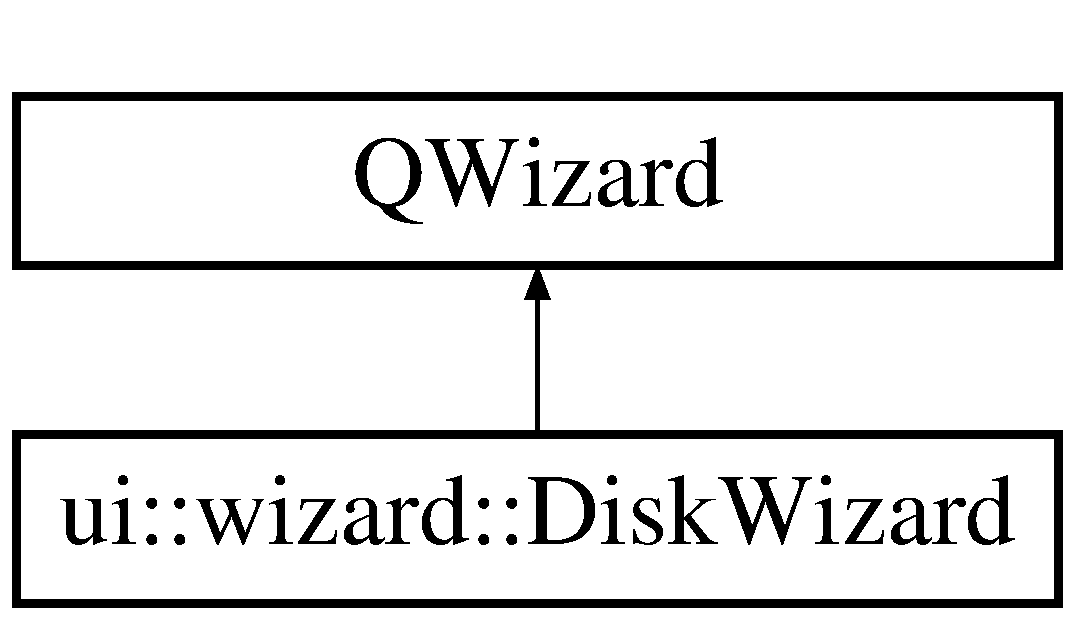
\includegraphics[height=2.000000cm]{classui_1_1wizard_1_1_disk_wizard}
\end{center}
\end{figure}
\subsection*{Public Member Functions}
\begin{DoxyCompactItemize}
\item 
\mbox{\hyperlink{classui_1_1wizard_1_1_disk_wizard_a728f3938ee8a8f44cef12158b6e6ab1f}{Disk\+Wizard}} (Q\+Widget $\ast$parent=nullptr)
\begin{DoxyCompactList}\small\item\em \mbox{\hyperlink{classui_1_1wizard_1_1_disk_wizard}{Disk\+Wizard}} Constructor. \end{DoxyCompactList}\item 
\mbox{\Hypertarget{classui_1_1wizard_1_1_disk_wizard_a9376442c638a808b79a27be0379f83c2}\label{classui_1_1wizard_1_1_disk_wizard_a9376442c638a808b79a27be0379f83c2}} 
virtual \mbox{\hyperlink{classui_1_1wizard_1_1_disk_wizard_a9376442c638a808b79a27be0379f83c2}{$\sim$\+Disk\+Wizard}} (void) override
\begin{DoxyCompactList}\small\item\em $\sim$\+Disk\+Wizard Destrucotr \end{DoxyCompactList}\item 
\mbox{\hyperlink{classcore_1_1disk_1_1_disk}{core\+::disk\+::\+Disk}} $\ast$ \mbox{\hyperlink{classui_1_1wizard_1_1_disk_wizard_ae62aaaaa962e9cac555928bf84579e8f}{get\+Resulted\+Disk}} (void)
\begin{DoxyCompactList}\small\item\em get\+Resulted\+Disk This method returns the disk which where created. \end{DoxyCompactList}\end{DoxyCompactItemize}
\subsection*{Protected Member Functions}
\begin{DoxyCompactItemize}
\item 
virtual void \mbox{\hyperlink{classui_1_1wizard_1_1_disk_wizard_aa0569c57c5568c9b03bbae99661f11ac}{done}} (int result) override
\begin{DoxyCompactList}\small\item\em done This is a custom implementation of the done event \end{DoxyCompactList}\end{DoxyCompactItemize}


\subsection{Detailed Description}
This class this class implements a wizard. 

This class is a custom implementation of a wizard. It handles all pages and serves as an interaction with the calling object \begin{DoxyAuthor}{Author}
Nils Milewski (10010480) 
\end{DoxyAuthor}


\subsection{Constructor \& Destructor Documentation}
\mbox{\Hypertarget{classui_1_1wizard_1_1_disk_wizard_a728f3938ee8a8f44cef12158b6e6ab1f}\label{classui_1_1wizard_1_1_disk_wizard_a728f3938ee8a8f44cef12158b6e6ab1f}} 
\index{ui\+::wizard\+::\+Disk\+Wizard@{ui\+::wizard\+::\+Disk\+Wizard}!Disk\+Wizard@{Disk\+Wizard}}
\index{Disk\+Wizard@{Disk\+Wizard}!ui\+::wizard\+::\+Disk\+Wizard@{ui\+::wizard\+::\+Disk\+Wizard}}
\subsubsection{\texorpdfstring{Disk\+Wizard()}{DiskWizard()}}
{\footnotesize\ttfamily Disk\+Wizard\+::\+Disk\+Wizard (\begin{DoxyParamCaption}\item[{Q\+Widget $\ast$}]{parent = {\ttfamily nullptr} }\end{DoxyParamCaption})}



\mbox{\hyperlink{classui_1_1wizard_1_1_disk_wizard}{Disk\+Wizard}} Constructor. 

This constructor construct a wizard and assign the page order. 
\begin{DoxyParams}{Parameters}
{\em parent} & \\
\hline
\end{DoxyParams}


\subsection{Member Function Documentation}
\mbox{\Hypertarget{classui_1_1wizard_1_1_disk_wizard_aa0569c57c5568c9b03bbae99661f11ac}\label{classui_1_1wizard_1_1_disk_wizard_aa0569c57c5568c9b03bbae99661f11ac}} 
\index{ui\+::wizard\+::\+Disk\+Wizard@{ui\+::wizard\+::\+Disk\+Wizard}!done@{done}}
\index{done@{done}!ui\+::wizard\+::\+Disk\+Wizard@{ui\+::wizard\+::\+Disk\+Wizard}}
\subsubsection{\texorpdfstring{done()}{done()}}
{\footnotesize\ttfamily void Disk\+Wizard\+::done (\begin{DoxyParamCaption}\item[{int}]{result }\end{DoxyParamCaption})\hspace{0.3cm}{\ttfamily [override]}, {\ttfamily [protected]}, {\ttfamily [virtual]}}



done This is a custom implementation of the done event 

This event will ensure that the wizard only closes after the user aproved it with an anwser of a close question. 
\begin{DoxyParams}{Parameters}
{\em result} & Qt internal \\
\hline
\end{DoxyParams}
\mbox{\Hypertarget{classui_1_1wizard_1_1_disk_wizard_ae62aaaaa962e9cac555928bf84579e8f}\label{classui_1_1wizard_1_1_disk_wizard_ae62aaaaa962e9cac555928bf84579e8f}} 
\index{ui\+::wizard\+::\+Disk\+Wizard@{ui\+::wizard\+::\+Disk\+Wizard}!get\+Resulted\+Disk@{get\+Resulted\+Disk}}
\index{get\+Resulted\+Disk@{get\+Resulted\+Disk}!ui\+::wizard\+::\+Disk\+Wizard@{ui\+::wizard\+::\+Disk\+Wizard}}
\subsubsection{\texorpdfstring{get\+Resulted\+Disk()}{getResultedDisk()}}
{\footnotesize\ttfamily \mbox{\hyperlink{classcore_1_1disk_1_1_disk}{core\+::disk\+::\+Disk}} $\ast$ Disk\+Wizard\+::get\+Resulted\+Disk (\begin{DoxyParamCaption}\item[{void}]{ }\end{DoxyParamCaption})}



get\+Resulted\+Disk This method returns the disk which where created. 

This method creates a new Disk based on prviuous entered information \begin{DoxyReturn}{Returns}
Disk based on previous information 
\end{DoxyReturn}


The documentation for this class was generated from the following files\+:\begin{DoxyCompactItemize}
\item 
ui/wizard/diskwizard.\+h\item 
ui/wizard/diskwizard.\+cpp\end{DoxyCompactItemize}

\hypertarget{classcore_1_1_i_file_system}{}\section{core\+:\+:I\+File\+System Class Reference}
\label{classcore_1_1_i_file_system}\index{core\+::\+I\+File\+System@{core\+::\+I\+File\+System}}
\subsection*{Public Member Functions}
\begin{DoxyCompactItemize}
\item 
\mbox{\Hypertarget{classcore_1_1_i_file_system_a6ce2b2c38629462050b9ec53eda0a248}\label{classcore_1_1_i_file_system_a6ce2b2c38629462050b9ec53eda0a248}} 
{\bfseries I\+File\+System} (long block\+Size, long block\+Count)
\item 
\mbox{\Hypertarget{classcore_1_1_i_file_system_a493334ffcc971d8319bd00a141dca6e5}\label{classcore_1_1_i_file_system_a493334ffcc971d8319bd00a141dca6e5}} 
long {\bfseries block\+Size} (void)
\item 
\mbox{\Hypertarget{classcore_1_1_i_file_system_abd457a1423ac45a0c2e1fb980120dbf5}\label{classcore_1_1_i_file_system_abd457a1423ac45a0c2e1fb980120dbf5}} 
long {\bfseries amount\+Blocks} (void)
\item 
\mbox{\Hypertarget{classcore_1_1_i_file_system_a00693ff330dde579f2ac4740903d9904}\label{classcore_1_1_i_file_system_a00693ff330dde579f2ac4740903d9904}} 
virtual void {\bfseries mount} (void)=0
\item 
\mbox{\Hypertarget{classcore_1_1_i_file_system_a1fc1e6c654103f93abcd307009b7b175}\label{classcore_1_1_i_file_system_a1fc1e6c654103f93abcd307009b7b175}} 
virtual void {\bfseries unmount} (void)=0
\item 
\mbox{\Hypertarget{classcore_1_1_i_file_system_a05a699c4bd1efafa91871b71d40dac7f}\label{classcore_1_1_i_file_system_a05a699c4bd1efafa91871b71d40dac7f}} 
virtual void {\bfseries self\+Check} (void)=0
\item 
\mbox{\Hypertarget{classcore_1_1_i_file_system_a4c968735ba948b62fcd401b9a4d0d76b}\label{classcore_1_1_i_file_system_a4c968735ba948b62fcd401b9a4d0d76b}} 
virtual void {\bfseries self\+Repair} (void)=0
\item 
\mbox{\Hypertarget{classcore_1_1_i_file_system_a1c197a52cb302e708a961fedfd0f2b4f}\label{classcore_1_1_i_file_system_a1c197a52cb302e708a961fedfd0f2b4f}} 
virtual void {\bfseries create\+File} (void)=0
\item 
\mbox{\Hypertarget{classcore_1_1_i_file_system_a2afdee3dd280f84415d6d0e8cf3c43b9}\label{classcore_1_1_i_file_system_a2afdee3dd280f84415d6d0e8cf3c43b9}} 
virtual void {\bfseries create\+Directory} (void)=0
\item 
\mbox{\Hypertarget{classcore_1_1_i_file_system_acbf35289019edc01a4ca8705e7894ec0}\label{classcore_1_1_i_file_system_acbf35289019edc01a4ca8705e7894ec0}} 
virtual void {\bfseries delete\+File} (void)=0
\item 
\mbox{\Hypertarget{classcore_1_1_i_file_system_a2aa404fe7bd033745a7e8a84a6f59e21}\label{classcore_1_1_i_file_system_a2aa404fe7bd033745a7e8a84a6f59e21}} 
virtual void {\bfseries delete\+Directory} (void)=0
\item 
\mbox{\Hypertarget{classcore_1_1_i_file_system_a79903fcc3d8c3e3cb42eebed7dd0b0f0}\label{classcore_1_1_i_file_system_a79903fcc3d8c3e3cb42eebed7dd0b0f0}} 
virtual void {\bfseries open\+File} (void)=0
\item 
\mbox{\Hypertarget{classcore_1_1_i_file_system_a85d426cd90b6f6bb437d64cf17303226}\label{classcore_1_1_i_file_system_a85d426cd90b6f6bb437d64cf17303226}} 
virtual void {\bfseries close\+File} (void)=0
\item 
\mbox{\Hypertarget{classcore_1_1_i_file_system_a2f3e927026b148bbefd9d44f3e1dfaef}\label{classcore_1_1_i_file_system_a2f3e927026b148bbefd9d44f3e1dfaef}} 
virtual const char $\ast$ {\bfseries read\+File} (void)=0
\item 
\mbox{\Hypertarget{classcore_1_1_i_file_system_adbcc31a9db94f4787620d326bc920d60}\label{classcore_1_1_i_file_system_adbcc31a9db94f4787620d326bc920d60}} 
virtual const char $\ast$ {\bfseries read\+File} (int length)=0
\item 
\mbox{\Hypertarget{classcore_1_1_i_file_system_ae1108a72181c1c304426e90ceda31d25}\label{classcore_1_1_i_file_system_ae1108a72181c1c304426e90ceda31d25}} 
virtual void {\bfseries write\+File} (const char $\ast$data, int length)=0
\item 
\mbox{\Hypertarget{classcore_1_1_i_file_system_ab55a79b54bc802aea7a013cb8c8914e8}\label{classcore_1_1_i_file_system_ab55a79b54bc802aea7a013cb8c8914e8}} 
virtual char {\bfseries fragmentation} (void)=0
\item 
\mbox{\Hypertarget{classcore_1_1_i_file_system_a6938f746c7a5f520884e746543d00658}\label{classcore_1_1_i_file_system_a6938f746c7a5f520884e746543d00658}} 
virtual void {\bfseries defrag} (void)=0
\item 
\mbox{\Hypertarget{classcore_1_1_i_file_system_ac2a36a24f58595213d43df9d7935a390}\label{classcore_1_1_i_file_system_ac2a36a24f58595213d43df9d7935a390}} 
virtual long {\bfseries free\+Space} (void)=0
\item 
\mbox{\Hypertarget{classcore_1_1_i_file_system_a88692a64f0e55150680b81c1db4eb020}\label{classcore_1_1_i_file_system_a88692a64f0e55150680b81c1db4eb020}} 
virtual long {\bfseries used\+Space} (void)=0
\item 
\mbox{\Hypertarget{classcore_1_1_i_file_system_a1051ca91a2c34231e437956a5a5b2acd}\label{classcore_1_1_i_file_system_a1051ca91a2c34231e437956a5a5b2acd}} 
virtual long {\bfseries capacity} (void)=0
\item 
\mbox{\Hypertarget{classcore_1_1_i_file_system_a117d4301045c1f8cb85290f5c73e5c8b}\label{classcore_1_1_i_file_system_a117d4301045c1f8cb85290f5c73e5c8b}} 
virtual void {\bfseries change\+Attributes} ()=0
\end{DoxyCompactItemize}
\subsection*{Private Attributes}
\begin{DoxyCompactItemize}
\item 
\mbox{\Hypertarget{classcore_1_1_i_file_system_a6fc974f16f1350e21941989075e01023}\label{classcore_1_1_i_file_system_a6fc974f16f1350e21941989075e01023}} 
long {\bfseries block\+Size\+\_\+m}
\item 
\mbox{\Hypertarget{classcore_1_1_i_file_system_ae87ddee28a5da64b90c2d197b83ed3c9}\label{classcore_1_1_i_file_system_ae87ddee28a5da64b90c2d197b83ed3c9}} 
long {\bfseries block\+Count\+\_\+m}
\end{DoxyCompactItemize}


The documentation for this class was generated from the following files\+:\begin{DoxyCompactItemize}
\item 
core/ifilesystem.\+h\item 
core/ifilesystem.\+cpp\end{DoxyCompactItemize}

\hypertarget{classui_1_1wizard_1_1pages_1_1_intro_page}{}\section{ui\+:\+:wizard\+:\+:pages\+:\+:Intro\+Page Class Reference}
\label{classui_1_1wizard_1_1pages_1_1_intro_page}\index{ui\+::wizard\+::pages\+::\+Intro\+Page@{ui\+::wizard\+::pages\+::\+Intro\+Page}}


This class provides a custom implementation of a wizard page.  




{\ttfamily \#include $<$intropage.\+h$>$}

Inheritance diagram for ui\+:\+:wizard\+:\+:pages\+:\+:Intro\+Page\+:\begin{figure}[H]
\begin{center}
\leavevmode
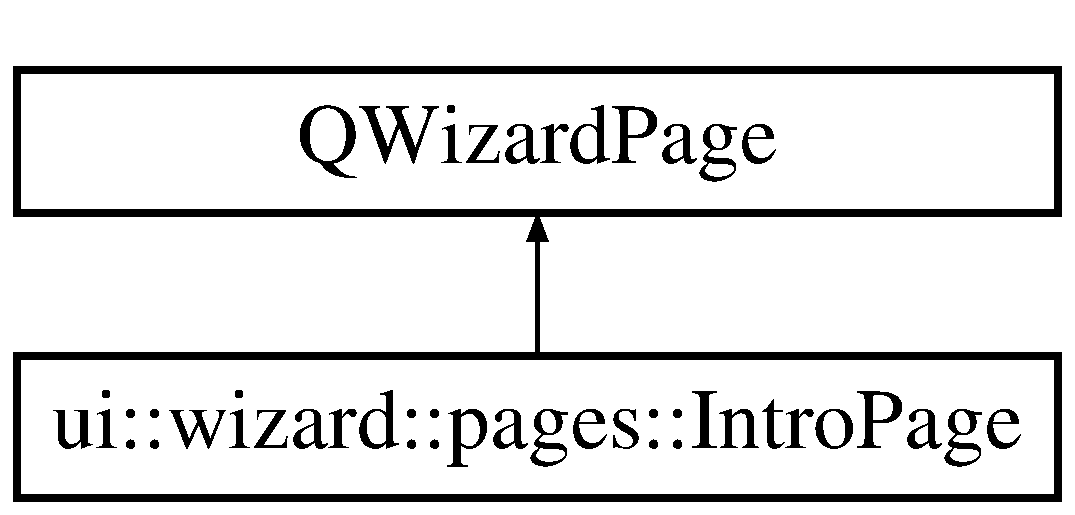
\includegraphics[height=2.000000cm]{classui_1_1wizard_1_1pages_1_1_intro_page}
\end{center}
\end{figure}
\subsection*{Public Member Functions}
\begin{DoxyCompactItemize}
\item 
\mbox{\hyperlink{classui_1_1wizard_1_1pages_1_1_intro_page_ad984d57f77f15e89e82d1184c997b778}{Intro\+Page}} (Q\+String text, \mbox{\hyperlink{namespaceui_1_1wizard_1_1pages_a1a25c157e498474f0cf868944a52bf44}{pages\+\_\+enum}} next\+Page, Q\+Widget $\ast$parent=nullptr)
\begin{DoxyCompactList}\small\item\em \mbox{\hyperlink{classui_1_1wizard_1_1pages_1_1_intro_page}{Intro\+Page}} This is a constructor. \end{DoxyCompactList}\item 
virtual \mbox{\hyperlink{classui_1_1wizard_1_1pages_1_1_intro_page_ac83805abea5b47093cc0e3ff4c85abf3}{$\sim$\+Intro\+Page}} (void) override
\begin{DoxyCompactList}\small\item\em $\sim$\+Intro\+Page Destructor \end{DoxyCompactList}\item 
int \mbox{\hyperlink{classui_1_1wizard_1_1pages_1_1_intro_page_a210708d731eaca79e5c0d220c08ad739}{next\+Id}} () const override
\begin{DoxyCompactList}\small\item\em next\+Id This method returns the next id \end{DoxyCompactList}\end{DoxyCompactItemize}
\subsection*{Private Attributes}
\begin{DoxyCompactItemize}
\item 
\mbox{\hyperlink{namespaceui_1_1wizard_1_1pages_a1a25c157e498474f0cf868944a52bf44}{pages\+\_\+enum}} \mbox{\hyperlink{classui_1_1wizard_1_1pages_1_1_intro_page_a8b77ec9feb8996a03d71f034ee3296ca}{next\+Page\+\_\+m}}
\begin{DoxyCompactList}\small\item\em next\+Page\+\_\+m This variable contains the next page, \end{DoxyCompactList}\end{DoxyCompactItemize}


\subsection{Detailed Description}
This class provides a custom implementation of a wizard page. 

This class is a custom implementation of a wizard page It provides a quick introduction about the following wizard steps \begin{DoxyAuthor}{Author}
Nils Milewski (10010480) 
\end{DoxyAuthor}


\subsection{Constructor \& Destructor Documentation}
\mbox{\Hypertarget{classui_1_1wizard_1_1pages_1_1_intro_page_ad984d57f77f15e89e82d1184c997b778}\label{classui_1_1wizard_1_1pages_1_1_intro_page_ad984d57f77f15e89e82d1184c997b778}} 
\index{ui\+::wizard\+::pages\+::\+Intro\+Page@{ui\+::wizard\+::pages\+::\+Intro\+Page}!Intro\+Page@{Intro\+Page}}
\index{Intro\+Page@{Intro\+Page}!ui\+::wizard\+::pages\+::\+Intro\+Page@{ui\+::wizard\+::pages\+::\+Intro\+Page}}
\subsubsection{\texorpdfstring{Intro\+Page()}{IntroPage()}}
{\footnotesize\ttfamily Intro\+Page\+::\+Intro\+Page (\begin{DoxyParamCaption}\item[{Q\+String}]{text,  }\item[{\mbox{\hyperlink{namespaceui_1_1wizard_1_1pages_a1a25c157e498474f0cf868944a52bf44}{pages\+\_\+enum}}}]{next\+Page,  }\item[{Q\+Widget $\ast$}]{parent = {\ttfamily nullptr} }\end{DoxyParamCaption})}



\mbox{\hyperlink{classui_1_1wizard_1_1pages_1_1_intro_page}{Intro\+Page}} This is a constructor. 

This constructor creates the layout of the page and set required attributes 
\begin{DoxyParams}{Parameters}
{\em text} & Text which should be displayed to the user \\
\hline
{\em next\+Page} & Enum from the next step \\
\hline
\end{DoxyParams}
\begin{DoxySeeAlso}{See also}
\mbox{\hyperlink{pages__enum_8h_source}{pages\+\_\+enum.\+h}} 
\end{DoxySeeAlso}

\begin{DoxyParams}{Parameters}
{\em parent} & Parent object which this object is associated with \\
\hline
\end{DoxyParams}
\mbox{\Hypertarget{classui_1_1wizard_1_1pages_1_1_intro_page_ac83805abea5b47093cc0e3ff4c85abf3}\label{classui_1_1wizard_1_1pages_1_1_intro_page_ac83805abea5b47093cc0e3ff4c85abf3}} 
\index{ui\+::wizard\+::pages\+::\+Intro\+Page@{ui\+::wizard\+::pages\+::\+Intro\+Page}!````~Intro\+Page@{$\sim$\+Intro\+Page}}
\index{````~Intro\+Page@{$\sim$\+Intro\+Page}!ui\+::wizard\+::pages\+::\+Intro\+Page@{ui\+::wizard\+::pages\+::\+Intro\+Page}}
\subsubsection{\texorpdfstring{$\sim$\+Intro\+Page()}{~IntroPage()}}
{\footnotesize\ttfamily Intro\+Page\+::$\sim$\+Intro\+Page (\begin{DoxyParamCaption}\item[{void}]{ }\end{DoxyParamCaption})\hspace{0.3cm}{\ttfamily [override]}, {\ttfamily [virtual]}}



$\sim$\+Intro\+Page Destructor 

This destructor will free up used resources 

\subsection{Member Function Documentation}
\mbox{\Hypertarget{classui_1_1wizard_1_1pages_1_1_intro_page_a210708d731eaca79e5c0d220c08ad739}\label{classui_1_1wizard_1_1pages_1_1_intro_page_a210708d731eaca79e5c0d220c08ad739}} 
\index{ui\+::wizard\+::pages\+::\+Intro\+Page@{ui\+::wizard\+::pages\+::\+Intro\+Page}!next\+Id@{next\+Id}}
\index{next\+Id@{next\+Id}!ui\+::wizard\+::pages\+::\+Intro\+Page@{ui\+::wizard\+::pages\+::\+Intro\+Page}}
\subsubsection{\texorpdfstring{next\+Id()}{nextId()}}
{\footnotesize\ttfamily int Intro\+Page\+::next\+Id (\begin{DoxyParamCaption}{ }\end{DoxyParamCaption}) const\hspace{0.3cm}{\ttfamily [override]}}



next\+Id This method returns the next id 

This method overrides the default implementation to utilize different intro pages. It will return the enum of next\+\_\+page to differenciate between disk and partition pages \begin{DoxyReturn}{Returns}
Next id for the wizard 
\end{DoxyReturn}


\subsection{Member Data Documentation}
\mbox{\Hypertarget{classui_1_1wizard_1_1pages_1_1_intro_page_a8b77ec9feb8996a03d71f034ee3296ca}\label{classui_1_1wizard_1_1pages_1_1_intro_page_a8b77ec9feb8996a03d71f034ee3296ca}} 
\index{ui\+::wizard\+::pages\+::\+Intro\+Page@{ui\+::wizard\+::pages\+::\+Intro\+Page}!next\+Page\+\_\+m@{next\+Page\+\_\+m}}
\index{next\+Page\+\_\+m@{next\+Page\+\_\+m}!ui\+::wizard\+::pages\+::\+Intro\+Page@{ui\+::wizard\+::pages\+::\+Intro\+Page}}
\subsubsection{\texorpdfstring{next\+Page\+\_\+m}{nextPage\_m}}
{\footnotesize\ttfamily \mbox{\hyperlink{namespaceui_1_1wizard_1_1pages_a1a25c157e498474f0cf868944a52bf44}{pages\+\_\+enum}} ui\+::wizard\+::pages\+::\+Intro\+Page\+::next\+Page\+\_\+m\hspace{0.3cm}{\ttfamily [private]}}



next\+Page\+\_\+m This variable contains the next page, 

next page containt the page index which should follow. You can look into \mbox{\hyperlink{pages__enum_8h_source}{pages\+\_\+enum.\+h}} for a detailed look about all possible pages. Most of the time it will be used to switch between disk and partition pages. 

The documentation for this class was generated from the following files\+:\begin{DoxyCompactItemize}
\item 
ui/wizard/pages/intropage.\+h\item 
ui/wizard/pages/intropage.\+cpp\end{DoxyCompactItemize}

\hypertarget{classui_1_1window_1_1_main_window}{}\section{ui\+:\+:window\+:\+:Main\+Window Class Reference}
\label{classui_1_1window_1_1_main_window}\index{ui\+::window\+::\+Main\+Window@{ui\+::window\+::\+Main\+Window}}


The \mbox{\hyperlink{classui_1_1window_1_1_main_window}{Main\+Window}} class.  




{\ttfamily \#include $<$mainwindow.\+h$>$}

Inheritance diagram for ui\+:\+:window\+:\+:Main\+Window\+:\begin{figure}[H]
\begin{center}
\leavevmode
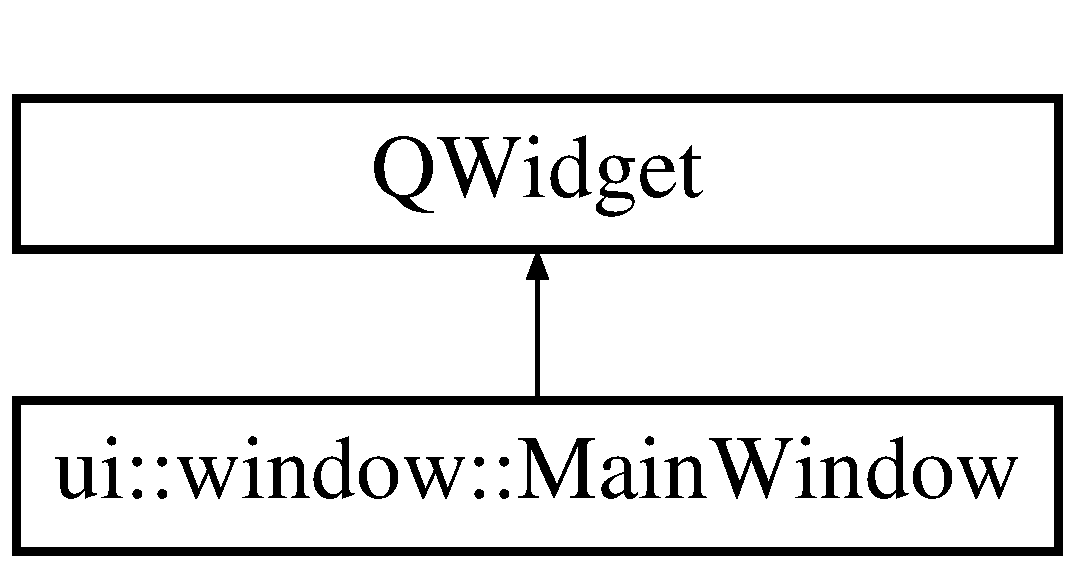
\includegraphics[height=2.000000cm]{classui_1_1window_1_1_main_window}
\end{center}
\end{figure}
\subsection*{Public Slots}
\begin{DoxyCompactItemize}
\item 
\mbox{\Hypertarget{classui_1_1window_1_1_main_window_a59fc90a3e94d7b3749a01420154b7180}\label{classui_1_1window_1_1_main_window_a59fc90a3e94d7b3749a01420154b7180}} 
void {\bfseries disk\+Pane\+Item\+Clicked} (Q\+List\+Widget\+Item $\ast$item)
\item 
\mbox{\Hypertarget{classui_1_1window_1_1_main_window_a1c0253c5f8350142145e647ba11b4eb5}\label{classui_1_1window_1_1_main_window_a1c0253c5f8350142145e647ba11b4eb5}} 
void {\bfseries click} ()
\item 
\mbox{\Hypertarget{classui_1_1window_1_1_main_window_a3c3e137427fb9ef9f774f08d40b98d7b}\label{classui_1_1window_1_1_main_window_a3c3e137427fb9ef9f774f08d40b98d7b}} 
void {\bfseries control\+Pane\+Item\+Clicked} (Q\+List\+Widget\+Item $\ast$item)
\item 
\mbox{\Hypertarget{classui_1_1window_1_1_main_window_a6b7db1a39889962fc97e0f8a0840ab4c}\label{classui_1_1window_1_1_main_window_a6b7db1a39889962fc97e0f8a0840ab4c}} 
void {\bfseries partition\+Pane\+Item\+Clicked} (Q\+List\+Widget\+Item $\ast$item)
\end{DoxyCompactItemize}
\subsection*{Public Member Functions}
\begin{DoxyCompactItemize}
\item 
\mbox{\Hypertarget{classui_1_1window_1_1_main_window_a770edeeb1dca0d8365f28ded5ac8c1a7}\label{classui_1_1window_1_1_main_window_a770edeeb1dca0d8365f28ded5ac8c1a7}} 
void {\bfseries refresh\+Disks} (void)
\item 
\mbox{\Hypertarget{classui_1_1window_1_1_main_window_a1e20191c2f6cecf881ed3a4de6147e12}\label{classui_1_1window_1_1_main_window_a1e20191c2f6cecf881ed3a4de6147e12}} 
void {\bfseries refresh\+Partition} (void)
\item 
\mbox{\Hypertarget{classui_1_1window_1_1_main_window_a8f650e410a52c007fbc62e13b09cceef}\label{classui_1_1window_1_1_main_window_a8f650e410a52c007fbc62e13b09cceef}} 
void {\bfseries refresh\+UI} ()
\end{DoxyCompactItemize}
\subsection*{Protected Member Functions}
\begin{DoxyCompactItemize}
\item 
\mbox{\Hypertarget{classui_1_1window_1_1_main_window_a5721fc9aa7fcc5727e137c8f4264db24}\label{classui_1_1window_1_1_main_window_a5721fc9aa7fcc5727e137c8f4264db24}} 
void {\bfseries hide\+Event} (Q\+Hide\+Event $\ast$event) override
\end{DoxyCompactItemize}
\subsection*{Private Attributes}
\begin{DoxyCompactItemize}
\item 
\mbox{\Hypertarget{classui_1_1window_1_1_main_window_a04cbd2f131266718a62c4330ccbaacee}\label{classui_1_1window_1_1_main_window_a04cbd2f131266718a62c4330ccbaacee}} 
\mbox{\hyperlink{classui_1_1window_1_1_detail_page}{Detail\+Page}} $\ast$ {\bfseries page}
\item 
\mbox{\Hypertarget{classui_1_1window_1_1_main_window_a96e1e831a4fdba02f811a4b06c6d4c44}\label{classui_1_1window_1_1_main_window_a96e1e831a4fdba02f811a4b06c6d4c44}} 
Q\+Tab\+Widget $\ast$ {\bfseries tab\+Widget}
\item 
\mbox{\Hypertarget{classui_1_1window_1_1_main_window_aa7325ee0fcf7d33b9065f69851122a0f}\label{classui_1_1window_1_1_main_window_aa7325ee0fcf7d33b9065f69851122a0f}} 
Q\+H\+Box\+Layout $\ast$ {\bfseries layout}
\item 
\mbox{\Hypertarget{classui_1_1window_1_1_main_window_a54496f7d21ae1ae510aafbeb837e0c1e}\label{classui_1_1window_1_1_main_window_a54496f7d21ae1ae510aafbeb837e0c1e}} 
Q\+H\+Box\+Layout $\ast$ {\bfseries detail\+Pane}
\item 
\mbox{\Hypertarget{classui_1_1window_1_1_main_window_a517b2e82838b0eab89ab089c1c7bfe01}\label{classui_1_1window_1_1_main_window_a517b2e82838b0eab89ab089c1c7bfe01}} 
\mbox{\hyperlink{classui_1_1custom_u_i_1_1_custom_control_bar}{ui\+::custom\+U\+I\+::\+Custom\+Control\+Bar}} $\ast$ {\bfseries tmp}
\item 
\mbox{\Hypertarget{classui_1_1window_1_1_main_window_aa00bcce6e063ac300b700aa5c7348259}\label{classui_1_1window_1_1_main_window_aa00bcce6e063ac300b700aa5c7348259}} 
Q\+List\+Widget $\ast$ {\bfseries disk\+Pane}
\item 
\mbox{\Hypertarget{classui_1_1window_1_1_main_window_ab2ba1f351c5f476c5ccbaeed683e90eb}\label{classui_1_1window_1_1_main_window_ab2ba1f351c5f476c5ccbaeed683e90eb}} 
Q\+List\+Widget\+Item $\ast$ {\bfseries current\+Disk}
\item 
\mbox{\Hypertarget{classui_1_1window_1_1_main_window_a88bebba612acbd3eec664693c0d9a722}\label{classui_1_1window_1_1_main_window_a88bebba612acbd3eec664693c0d9a722}} 
Q\+List\+Widget $\ast$ {\bfseries partition\+Pane}
\item 
\mbox{\Hypertarget{classui_1_1window_1_1_main_window_aa29b3eeaa0ca10708a642a199d09c990}\label{classui_1_1window_1_1_main_window_aa29b3eeaa0ca10708a642a199d09c990}} 
Q\+List\+Widget\+Item $\ast$ {\bfseries current\+Partition}
\item 
\mbox{\Hypertarget{classui_1_1window_1_1_main_window_a1cbe56c915e49bbe6deecc8748472cea}\label{classui_1_1window_1_1_main_window_a1cbe56c915e49bbe6deecc8748472cea}} 
Q\+List\+Widget $\ast$ {\bfseries tool\+Pane}
\item 
\mbox{\Hypertarget{classui_1_1window_1_1_main_window_a03223362f26005b9c351eab066c1a7d5}\label{classui_1_1window_1_1_main_window_a03223362f26005b9c351eab066c1a7d5}} 
Q\+List\+Widget\+Item $\ast$ {\bfseries current\+Tool}
\item 
\mbox{\Hypertarget{classui_1_1window_1_1_main_window_ab2ab4d5f6ee5536275458c4808827b1c}\label{classui_1_1window_1_1_main_window_ab2ab4d5f6ee5536275458c4808827b1c}} 
\mbox{\hyperlink{classui_1_1custom_u_i_1_1_custom_list_widget_item}{ui\+::custom\+U\+I\+::\+Custom\+List\+Widget\+Item}} $\ast$ {\bfseries root\+Item}
\item 
\mbox{\Hypertarget{classui_1_1window_1_1_main_window_a8c4aeb9590f059a4c2b8173354f1045f}\label{classui_1_1window_1_1_main_window_a8c4aeb9590f059a4c2b8173354f1045f}} 
\mbox{\hyperlink{classui_1_1custom_u_i_1_1_custom_list_widget_item}{ui\+::custom\+U\+I\+::\+Custom\+List\+Widget\+Item}} $\ast$ {\bfseries disk\+Info\+Item}
\item 
\mbox{\Hypertarget{classui_1_1window_1_1_main_window_a8f927ac7149efbea7fe51fb6552d9b51}\label{classui_1_1window_1_1_main_window_a8f927ac7149efbea7fe51fb6552d9b51}} 
\mbox{\hyperlink{classui_1_1custom_u_i_1_1_custom_list_widget_item}{ui\+::custom\+U\+I\+::\+Custom\+List\+Widget\+Item}} $\ast$ {\bfseries resize\+Item}
\item 
\mbox{\Hypertarget{classui_1_1window_1_1_main_window_ab4386fa5b81b950f86703493c8a15521}\label{classui_1_1window_1_1_main_window_ab4386fa5b81b950f86703493c8a15521}} 
\mbox{\hyperlink{classui_1_1custom_u_i_1_1_custom_list_widget_item}{ui\+::custom\+U\+I\+::\+Custom\+List\+Widget\+Item}} $\ast$ {\bfseries add\+Partition}
\item 
\mbox{\Hypertarget{classui_1_1window_1_1_main_window_abb9c3b148ed4962768f35d43f8bdb7ca}\label{classui_1_1window_1_1_main_window_abb9c3b148ed4962768f35d43f8bdb7ca}} 
std\+::vector$<$ \mbox{\hyperlink{classcore_1_1disk_1_1_disk}{core\+::disk\+::\+Disk}} $\ast$ $>$ $\ast$ {\bfseries disks}
\item 
\mbox{\Hypertarget{classui_1_1window_1_1_main_window_a1ebb4730f1b18ab3cbf672d3651006e8}\label{classui_1_1window_1_1_main_window_a1ebb4730f1b18ab3cbf672d3651006e8}} 
\mbox{\hyperlink{classcore_1_1disk_1_1_disk}{core\+::disk\+::\+Disk}} $\ast$ {\bfseries working\+Disk}
\end{DoxyCompactItemize}


\subsection{Detailed Description}
The \mbox{\hyperlink{classui_1_1window_1_1_main_window}{Main\+Window}} class. 

The documentation for this class was generated from the following files\+:\begin{DoxyCompactItemize}
\item 
ui/pages/mainwindow.\+h\item 
ui/pages/mainwindow.\+cpp\end{DoxyCompactItemize}

\hypertarget{classcore_1_1disk_1_1_master_boot_record}{}\section{core\+:\+:disk\+:\+:Master\+Boot\+Record Class Reference}
\label{classcore_1_1disk_1_1_master_boot_record}\index{core\+::disk\+::\+Master\+Boot\+Record@{core\+::disk\+::\+Master\+Boot\+Record}}


The \mbox{\hyperlink{classcore_1_1disk_1_1_master_boot_record}{Master\+Boot\+Record}} class.  




{\ttfamily \#include $<$masterbootrecord.\+h$>$}

\subsection*{Public Member Functions}
\begin{DoxyCompactItemize}
\item 
\mbox{\hyperlink{classcore_1_1disk_1_1_master_boot_record_ad037f4c38e76f64b7d06f8795531442c}{Master\+Boot\+Record}} (unsigned long long disk\+Capacity)
\begin{DoxyCompactList}\small\item\em \mbox{\hyperlink{classcore_1_1disk_1_1_master_boot_record}{Master\+Boot\+Record}} Constructor. \end{DoxyCompactList}\item 
\mbox{\hyperlink{classcore_1_1logic_1_1_partition}{logic\+::\+Partition}} $\ast$ \mbox{\hyperlink{classcore_1_1disk_1_1_master_boot_record_a857825face8484c5bbc23768cd4344d6}{get\+Partition}} (int index)
\begin{DoxyCompactList}\small\item\em get\+Partition This method queries a partition from the Master Boot Record \end{DoxyCompactList}\item 
bool \mbox{\hyperlink{classcore_1_1disk_1_1_master_boot_record_ab1f46cc41735db1fcdd2aef912da29a4}{add\+Partition}} (long block\+Size, long amount\+Blocks, \mbox{\hyperlink{classcore_1_1_i_file_system}{I\+File\+System}} $\ast$file\+System)
\begin{DoxyCompactList}\small\item\em add\+Partition Adds a new partition to the M\+BR \end{DoxyCompactList}\item 
bool \mbox{\hyperlink{classcore_1_1disk_1_1_master_boot_record_a901d6bfb4b860b739e204be4f6cc47a4}{add\+Partition}} (int index, long block\+Size, long amount\+Blocks, \mbox{\hyperlink{classcore_1_1_i_file_system}{I\+File\+System}} $\ast$file\+System)
\begin{DoxyCompactList}\small\item\em add\+Partition Adds a new partition to the M\+BR \end{DoxyCompactList}\item 
bool \mbox{\hyperlink{classcore_1_1disk_1_1_master_boot_record_af155df4b9738c217678a8f875e679c50}{remove\+Partition}} (int index)
\begin{DoxyCompactList}\small\item\em remove\+Partition Removes a partition \end{DoxyCompactList}\item 
\mbox{\Hypertarget{classcore_1_1disk_1_1_master_boot_record_a87a82e1edd865a766f6cf73de147a9e1}\label{classcore_1_1disk_1_1_master_boot_record_a87a82e1edd865a766f6cf73de147a9e1}} 
unsigned long long {\bfseries available\+Space} (void)
\item 
\mbox{\Hypertarget{classcore_1_1disk_1_1_master_boot_record_a2247447acf2ad887c9ef1effbd397fae}\label{classcore_1_1disk_1_1_master_boot_record_a2247447acf2ad887c9ef1effbd397fae}} 
bool {\bfseries add\+Partition} (\mbox{\hyperlink{classcore_1_1logic_1_1_partition}{logic\+::\+Partition}} $\ast$partition)
\end{DoxyCompactItemize}
\subsection*{Static Public Attributes}
\begin{DoxyCompactItemize}
\item 
\mbox{\Hypertarget{classcore_1_1disk_1_1_master_boot_record_a8db81e19979e90b3f826745c9a14288b}\label{classcore_1_1disk_1_1_master_boot_record_a8db81e19979e90b3f826745c9a14288b}} 
static const int \mbox{\hyperlink{classcore_1_1disk_1_1_master_boot_record_a8db81e19979e90b3f826745c9a14288b}{M\+A\+X\+\_\+\+P\+A\+R\+T\+I\+T\+I\+ON}} = 4
\begin{DoxyCompactList}\small\item\em M\+A\+X\+\_\+\+P\+A\+R\+T\+I\+T\+I\+ON This variable contains the maximum of available partition. \end{DoxyCompactList}\end{DoxyCompactItemize}
\subsection*{Private Attributes}
\begin{DoxyCompactItemize}
\item 
\mbox{\Hypertarget{classcore_1_1disk_1_1_master_boot_record_ab332516409a1180967132f0a5249e3e6}\label{classcore_1_1disk_1_1_master_boot_record_ab332516409a1180967132f0a5249e3e6}} 
\mbox{\hyperlink{classcore_1_1logic_1_1_partition}{logic\+::\+Partition}} $\ast$ \mbox{\hyperlink{classcore_1_1disk_1_1_master_boot_record_ab332516409a1180967132f0a5249e3e6}{partitions\+\_\+m}} \mbox{[}\mbox{\hyperlink{classcore_1_1disk_1_1_master_boot_record_a8db81e19979e90b3f826745c9a14288b}{M\+A\+X\+\_\+\+P\+A\+R\+T\+I\+T\+I\+ON}}\mbox{]}
\begin{DoxyCompactList}\small\item\em partitions\+\_\+m This attribute is array of all registred partitions \end{DoxyCompactList}\item 
\mbox{\Hypertarget{classcore_1_1disk_1_1_master_boot_record_a133c97daafd6f7abd543f99a72744578}\label{classcore_1_1disk_1_1_master_boot_record_a133c97daafd6f7abd543f99a72744578}} 
unsigned long long \mbox{\hyperlink{classcore_1_1disk_1_1_master_boot_record_a133c97daafd6f7abd543f99a72744578}{disk\+Capacity\+\_\+m}}
\begin{DoxyCompactList}\small\item\em disk\+Capacity\+\_\+m This attributes contains the size of the disk \end{DoxyCompactList}\item 
\mbox{\Hypertarget{classcore_1_1disk_1_1_master_boot_record_a1e70503a01c4c4511050ca8e5173c43e}\label{classcore_1_1disk_1_1_master_boot_record_a1e70503a01c4c4511050ca8e5173c43e}} 
unsigned long long \mbox{\hyperlink{classcore_1_1disk_1_1_master_boot_record_a1e70503a01c4c4511050ca8e5173c43e}{available\+Disk\+Capacity\+\_\+m}}
\begin{DoxyCompactList}\small\item\em available\+Disk\+Capacity\+\_\+m This attributes contains the available size of the disk \end{DoxyCompactList}\end{DoxyCompactItemize}
\subsection*{Friends}
\begin{DoxyCompactItemize}
\item 
\mbox{\Hypertarget{classcore_1_1disk_1_1_master_boot_record_a33e3ea037895ea6142548552beee358a}\label{classcore_1_1disk_1_1_master_boot_record_a33e3ea037895ea6142548552beee358a}} 
std\+::ostream \& {\bfseries operator$<$$<$} (std\+::ostream \&os, \mbox{\hyperlink{classcore_1_1disk_1_1_master_boot_record}{Master\+Boot\+Record}} \&mbr)
\end{DoxyCompactItemize}


\subsection{Detailed Description}
The \mbox{\hyperlink{classcore_1_1disk_1_1_master_boot_record}{Master\+Boot\+Record}} class. 

This class represent a Master Boot Record entry \begin{DoxyAuthor}{Author}
Nils Milewski (10010480) 
\end{DoxyAuthor}


\subsection{Constructor \& Destructor Documentation}
\mbox{\Hypertarget{classcore_1_1disk_1_1_master_boot_record_ad037f4c38e76f64b7d06f8795531442c}\label{classcore_1_1disk_1_1_master_boot_record_ad037f4c38e76f64b7d06f8795531442c}} 
\index{core\+::disk\+::\+Master\+Boot\+Record@{core\+::disk\+::\+Master\+Boot\+Record}!Master\+Boot\+Record@{Master\+Boot\+Record}}
\index{Master\+Boot\+Record@{Master\+Boot\+Record}!core\+::disk\+::\+Master\+Boot\+Record@{core\+::disk\+::\+Master\+Boot\+Record}}
\subsubsection{\texorpdfstring{Master\+Boot\+Record()}{MasterBootRecord()}}
{\footnotesize\ttfamily Master\+Boot\+Record\+::\+Master\+Boot\+Record (\begin{DoxyParamCaption}\item[{unsigned long long}]{disk\+Capacity }\end{DoxyParamCaption})}



\mbox{\hyperlink{classcore_1_1disk_1_1_master_boot_record}{Master\+Boot\+Record}} Constructor. 

This Constructor sets the disk capacity and creates the array of partitions (partitions\+\_\+m) with null pointer 
\begin{DoxyParams}{Parameters}
{\em disk\+Capacity} & \\
\hline
\end{DoxyParams}


\subsection{Member Function Documentation}
\mbox{\Hypertarget{classcore_1_1disk_1_1_master_boot_record_ab1f46cc41735db1fcdd2aef912da29a4}\label{classcore_1_1disk_1_1_master_boot_record_ab1f46cc41735db1fcdd2aef912da29a4}} 
\index{core\+::disk\+::\+Master\+Boot\+Record@{core\+::disk\+::\+Master\+Boot\+Record}!add\+Partition@{add\+Partition}}
\index{add\+Partition@{add\+Partition}!core\+::disk\+::\+Master\+Boot\+Record@{core\+::disk\+::\+Master\+Boot\+Record}}
\subsubsection{\texorpdfstring{add\+Partition()}{addPartition()}\hspace{0.1cm}{\footnotesize\ttfamily [1/2]}}
{\footnotesize\ttfamily bool Master\+Boot\+Record\+::add\+Partition (\begin{DoxyParamCaption}\item[{long}]{block\+Size,  }\item[{long}]{amount\+Blocks,  }\item[{\mbox{\hyperlink{classcore_1_1_i_file_system}{I\+File\+System}} $\ast$}]{file\+System }\end{DoxyParamCaption})}



add\+Partition Adds a new partition to the M\+BR 

First a check if enough space is available is done. Next the M\+BR iterates over all entries from his partition table, iff the M\+BR finds a free spot (entry is nullptr) the M\+BR creates a new partition and returns true otherwise the M\+BR iterates to the end if all entries are used (not nullptr) false will be returned. 
\begin{DoxyParams}{Parameters}
{\em block\+Size} & Size of the block in bytes \\
\hline
{\em amount\+Blocks} & Amount of blocks the partition owns \\
\hline
{\em file\+System} & Filesystem of the Partition \\
\hline
\end{DoxyParams}
\begin{DoxyReturn}{Returns}
true if the Partition was created otherwise false 
\end{DoxyReturn}
\mbox{\Hypertarget{classcore_1_1disk_1_1_master_boot_record_a901d6bfb4b860b739e204be4f6cc47a4}\label{classcore_1_1disk_1_1_master_boot_record_a901d6bfb4b860b739e204be4f6cc47a4}} 
\index{core\+::disk\+::\+Master\+Boot\+Record@{core\+::disk\+::\+Master\+Boot\+Record}!add\+Partition@{add\+Partition}}
\index{add\+Partition@{add\+Partition}!core\+::disk\+::\+Master\+Boot\+Record@{core\+::disk\+::\+Master\+Boot\+Record}}
\subsubsection{\texorpdfstring{add\+Partition()}{addPartition()}\hspace{0.1cm}{\footnotesize\ttfamily [2/2]}}
{\footnotesize\ttfamily bool Master\+Boot\+Record\+::add\+Partition (\begin{DoxyParamCaption}\item[{int}]{index,  }\item[{long}]{block\+Size,  }\item[{long}]{amount\+Blocks,  }\item[{\mbox{\hyperlink{classcore_1_1_i_file_system}{I\+File\+System}} $\ast$}]{file\+System }\end{DoxyParamCaption})}



add\+Partition Adds a new partition to the M\+BR 

First a check if enough space is available is done. Next the M\+BR tries to insert a new Partition at given index, iff the spoti a free spot (entry is nullptr) the M\+BR creates a new partition and returns true otherwise the M\+BR false will be returned. 
\begin{DoxyParams}{Parameters}
{\em index} & Index where the partition should be located, range 0 -\/ 3 \\
\hline
{\em block\+Size} & Size of the block in bytes \\
\hline
{\em amount\+Blocks} & Amount of blocks the partition owns \\
\hline
{\em file\+System} & Filesystem of the Partition \\
\hline
\end{DoxyParams}
\begin{DoxyReturn}{Returns}
true if the Partition was created otherwise false 
\end{DoxyReturn}
\mbox{\Hypertarget{classcore_1_1disk_1_1_master_boot_record_a857825face8484c5bbc23768cd4344d6}\label{classcore_1_1disk_1_1_master_boot_record_a857825face8484c5bbc23768cd4344d6}} 
\index{core\+::disk\+::\+Master\+Boot\+Record@{core\+::disk\+::\+Master\+Boot\+Record}!get\+Partition@{get\+Partition}}
\index{get\+Partition@{get\+Partition}!core\+::disk\+::\+Master\+Boot\+Record@{core\+::disk\+::\+Master\+Boot\+Record}}
\subsubsection{\texorpdfstring{get\+Partition()}{getPartition()}}
{\footnotesize\ttfamily \mbox{\hyperlink{classcore_1_1logic_1_1_partition}{core\+::logic\+::\+Partition}} $\ast$ Master\+Boot\+Record\+::get\+Partition (\begin{DoxyParamCaption}\item[{int}]{index }\end{DoxyParamCaption})}



get\+Partition This method queries a partition from the Master Boot Record 

First a check about the index will be done, iff the index is out of range a exception will be thrown. Next a nullpointer check will be done, iff index argument points to a nullpointer entry a exception will be thrown. Iff all checks are done without an exceptiont the querried partition will be returned 
\begin{DoxyParams}{Parameters}
{\em index} & Index to access, range form 0 to 3 \\
\hline
\end{DoxyParams}
\begin{DoxyReturn}{Returns}
Partition assoziated with index Index 
\end{DoxyReturn}

\begin{DoxyExceptions}{Exceptions}
{\em runtime} & error if the index is out of range or the access would be a nullpointer \\
\hline
\end{DoxyExceptions}
\mbox{\Hypertarget{classcore_1_1disk_1_1_master_boot_record_af155df4b9738c217678a8f875e679c50}\label{classcore_1_1disk_1_1_master_boot_record_af155df4b9738c217678a8f875e679c50}} 
\index{core\+::disk\+::\+Master\+Boot\+Record@{core\+::disk\+::\+Master\+Boot\+Record}!remove\+Partition@{remove\+Partition}}
\index{remove\+Partition@{remove\+Partition}!core\+::disk\+::\+Master\+Boot\+Record@{core\+::disk\+::\+Master\+Boot\+Record}}
\subsubsection{\texorpdfstring{remove\+Partition()}{removePartition()}}
{\footnotesize\ttfamily bool Master\+Boot\+Record\+::remove\+Partition (\begin{DoxyParamCaption}\item[{int}]{index }\end{DoxyParamCaption})}



remove\+Partition Removes a partition 

This method removes a partiton at given index. First a check will be done to ensure that the index is not out of range(0 -\/ 3), if its out of range a runtimeexception will be thrown Next a check will be done to ensure that the partition is not a nullpoint, if its a nullpointer a runtimeexception will be trhown Iff all checks are done without an exception the partiton will be removed using his destructor and assign a nullpointer to the spot inside the partition table 
\begin{DoxyParams}{Parameters}
{\em index} & \\
\hline
\end{DoxyParams}
\begin{DoxyReturn}{Returns}

\end{DoxyReturn}


The documentation for this class was generated from the following files\+:\begin{DoxyCompactItemize}
\item 
core/masterbootrecord.\+h\item 
core/masterbootrecord.\+cpp\end{DoxyCompactItemize}

\hypertarget{classcore_1_1logic_1_1_partition}{}\section{core\+:\+:logic\+:\+:Partition Class Reference}
\label{classcore_1_1logic_1_1_partition}\index{core\+::logic\+::\+Partition@{core\+::logic\+::\+Partition}}


The \mbox{\hyperlink{classcore_1_1logic_1_1_partition}{Partition}} class.  




{\ttfamily \#include $<$partition.\+h$>$}

\subsection*{Public Member Functions}
\begin{DoxyCompactItemize}
\item 
\mbox{\hyperlink{classcore_1_1logic_1_1_partition_ad4a50cfda17b7996c8b1480e8701cf3a}{Partition}} (unsigned long long \mbox{\hyperlink{classcore_1_1logic_1_1_partition_ad3fb03e884170c6068b6724f1121ecc6}{block\+Size}}, unsigned long long \mbox{\hyperlink{classcore_1_1logic_1_1_partition_a28f8b672dccb67a06036e223be813950}{amount\+Blocks}}, \mbox{\hyperlink{classcore_1_1_i_file_system}{I\+File\+System}} $\ast$\mbox{\hyperlink{classcore_1_1logic_1_1_partition_a37dd86b3bc84bc1c7463beaf6d3adc57}{file\+System}})
\begin{DoxyCompactList}\small\item\em \mbox{\hyperlink{classcore_1_1logic_1_1_partition}{Partition}} Constructor. \end{DoxyCompactList}\item 
bool \mbox{\hyperlink{classcore_1_1logic_1_1_partition_a6530ca85e608e3af7243ac2b32e4c4e5}{format}} (unsigned long long \mbox{\hyperlink{classcore_1_1logic_1_1_partition_ad3fb03e884170c6068b6724f1121ecc6}{block\+Size}}, unsigned long long \mbox{\hyperlink{classcore_1_1logic_1_1_partition_a28f8b672dccb67a06036e223be813950}{amount\+Blocks}}, \mbox{\hyperlink{classcore_1_1_i_file_system}{I\+File\+System}} $\ast$\mbox{\hyperlink{classcore_1_1logic_1_1_partition_a37dd86b3bc84bc1c7463beaf6d3adc57}{file\+System}})
\begin{DoxyCompactList}\small\item\em format This method formats the partition \end{DoxyCompactList}\item 
bool \mbox{\hyperlink{classcore_1_1logic_1_1_partition_a43ea90c84d2d9b90e665efbc06d5d626}{erase}} (void)
\begin{DoxyCompactList}\small\item\em erase This method erased the partition \end{DoxyCompactList}\item 
unsigned long long \mbox{\hyperlink{classcore_1_1logic_1_1_partition_ad3fb03e884170c6068b6724f1121ecc6}{block\+Size}} (void)
\begin{DoxyCompactList}\small\item\em block\+Size getter of block size \end{DoxyCompactList}\item 
unsigned long long \mbox{\hyperlink{classcore_1_1logic_1_1_partition_a28f8b672dccb67a06036e223be813950}{amount\+Blocks}} (void)
\begin{DoxyCompactList}\small\item\em amount\+Blocks getter of amount block \end{DoxyCompactList}\item 
\mbox{\hyperlink{classcore_1_1_i_file_system}{I\+File\+System}} $\ast$ \mbox{\hyperlink{classcore_1_1logic_1_1_partition_a37dd86b3bc84bc1c7463beaf6d3adc57}{file\+System}} (void)
\begin{DoxyCompactList}\small\item\em file\+System getter of file system \end{DoxyCompactList}\item 
\mbox{\Hypertarget{classcore_1_1logic_1_1_partition_adeee9ac61d563134c5c1157d5e8d80d5}\label{classcore_1_1logic_1_1_partition_adeee9ac61d563134c5c1157d5e8d80d5}} 
void \mbox{\hyperlink{classcore_1_1logic_1_1_partition_adeee9ac61d563134c5c1157d5e8d80d5}{mount}} (void)
\begin{DoxyCompactList}\small\item\em mount This method mounts the partition and sets the mounted\+\_\+m attribute to true \end{DoxyCompactList}\item 
\mbox{\Hypertarget{classcore_1_1logic_1_1_partition_adc87e31edb60281d230acdf4bd972848}\label{classcore_1_1logic_1_1_partition_adc87e31edb60281d230acdf4bd972848}} 
void \mbox{\hyperlink{classcore_1_1logic_1_1_partition_adc87e31edb60281d230acdf4bd972848}{unmount}} (void)
\begin{DoxyCompactList}\small\item\em mount This method unmounts the partition and sets the mounted\+\_\+m attribute to false \end{DoxyCompactList}\item 
bool \mbox{\hyperlink{classcore_1_1logic_1_1_partition_a2278f8791ff716985ea54bd61470d96f}{is\+Mounted}} (void)
\begin{DoxyCompactList}\small\item\em mount This method determines if the partition is mounted. \end{DoxyCompactList}\item 
void \mbox{\hyperlink{classcore_1_1logic_1_1_partition_ab7b1a0f3847b9117a284cf4022e05e88}{resize}} (unsigned long long new\+Size)
\begin{DoxyCompactList}\small\item\em resize This method resizes the partition \end{DoxyCompactList}\end{DoxyCompactItemize}
\subsection*{Private Member Functions}
\begin{DoxyCompactItemize}
\item 
\mbox{\hyperlink{classcore_1_1logic_1_1_partition_acb291b3b0ccf48005e141be32fdd7efd}{Partition}} (\mbox{\hyperlink{classcore_1_1logic_1_1_partition}{Partition}} $\ast$partition)
\begin{DoxyCompactList}\small\item\em \mbox{\hyperlink{classcore_1_1logic_1_1_partition}{Partition}} Copy Constructor. \end{DoxyCompactList}\item 
\mbox{\hyperlink{classcore_1_1logic_1_1_partition_a019dc9e3d0c13954cd5d72f2049f21fd}{Partition}} (\mbox{\hyperlink{classcore_1_1logic_1_1_partition}{Partition}} \&partition)
\begin{DoxyCompactList}\small\item\em \mbox{\hyperlink{classcore_1_1logic_1_1_partition}{Partition}} Copy Constructor. \end{DoxyCompactList}\end{DoxyCompactItemize}
\subsection*{Private Attributes}
\begin{DoxyCompactItemize}
\item 
\mbox{\Hypertarget{classcore_1_1logic_1_1_partition_a57332acda5675a2f957f9dae15cb95ce}\label{classcore_1_1logic_1_1_partition_a57332acda5675a2f957f9dae15cb95ce}} 
unsigned long long \mbox{\hyperlink{classcore_1_1logic_1_1_partition_a57332acda5675a2f957f9dae15cb95ce}{block\+Size\+\_\+m}}
\begin{DoxyCompactList}\small\item\em block\+Size\+\_\+m Size of each block \end{DoxyCompactList}\item 
\mbox{\Hypertarget{classcore_1_1logic_1_1_partition_a373c1aa0747a05cf2cce5e52f45190f0}\label{classcore_1_1logic_1_1_partition_a373c1aa0747a05cf2cce5e52f45190f0}} 
unsigned long long \mbox{\hyperlink{classcore_1_1logic_1_1_partition_a373c1aa0747a05cf2cce5e52f45190f0}{amount\+Blocks\+\_\+m}}
\begin{DoxyCompactList}\small\item\em amount\+Blocks\+\_\+m Amount of used blocks \end{DoxyCompactList}\item 
\mbox{\Hypertarget{classcore_1_1logic_1_1_partition_a46f21abe3e81b2abf000c7d7c745d9dd}\label{classcore_1_1logic_1_1_partition_a46f21abe3e81b2abf000c7d7c745d9dd}} 
std\+::list$<$ \mbox{\hyperlink{classcore_1_1logic_1_1_block}{Block}} $\ast$ $>$ $\ast$ \mbox{\hyperlink{classcore_1_1logic_1_1_partition_a46f21abe3e81b2abf000c7d7c745d9dd}{blocks\+\_\+m}}
\begin{DoxyCompactList}\small\item\em blocks\+\_\+m The actual blocks \end{DoxyCompactList}\item 
\mbox{\Hypertarget{classcore_1_1logic_1_1_partition_a7f3c15de42e1b59f74f216cd382545d4}\label{classcore_1_1logic_1_1_partition_a7f3c15de42e1b59f74f216cd382545d4}} 
\mbox{\hyperlink{classcore_1_1_i_file_system}{I\+File\+System}} $\ast$ \mbox{\hyperlink{classcore_1_1logic_1_1_partition_a7f3c15de42e1b59f74f216cd382545d4}{file\+System\+\_\+m}}
\begin{DoxyCompactList}\small\item\em file\+System\+\_\+m The used filesystem(\+I\+Node, F\+A\+T) \end{DoxyCompactList}\item 
\mbox{\Hypertarget{classcore_1_1logic_1_1_partition_a1d5f9ed9365a32e9b78b6d9329b80b04}\label{classcore_1_1logic_1_1_partition_a1d5f9ed9365a32e9b78b6d9329b80b04}} 
bool \mbox{\hyperlink{classcore_1_1logic_1_1_partition_a1d5f9ed9365a32e9b78b6d9329b80b04}{mounted\+\_\+m}}
\begin{DoxyCompactList}\small\item\em mounted\+\_\+m States if the partition is mounted or not \end{DoxyCompactList}\end{DoxyCompactItemize}
\subsection*{Friends}
\begin{DoxyCompactItemize}
\item 
\mbox{\Hypertarget{classcore_1_1logic_1_1_partition_a9182c56fedac445f5d17d76f2efc9896}\label{classcore_1_1logic_1_1_partition_a9182c56fedac445f5d17d76f2efc9896}} 
std\+::ostream \& {\bfseries operator$<$$<$} (std\+::ostream \&os, \mbox{\hyperlink{classcore_1_1logic_1_1_partition}{Partition}} \&partition)
\end{DoxyCompactItemize}


\subsection{Detailed Description}
The \mbox{\hyperlink{classcore_1_1logic_1_1_partition}{Partition}} class. 

This class represent a partition with all required attributes and method. A partition contains the block information(size and amount) as well as the blocks itself. It also contains a file system and can be mounted. The partition can be formated and erased, as well as mounted and unmounted \begin{DoxyAuthor}{Author}
Nils Milewski (10010480) 
\end{DoxyAuthor}


\subsection{Constructor \& Destructor Documentation}
\mbox{\Hypertarget{classcore_1_1logic_1_1_partition_acb291b3b0ccf48005e141be32fdd7efd}\label{classcore_1_1logic_1_1_partition_acb291b3b0ccf48005e141be32fdd7efd}} 
\index{core\+::logic\+::\+Partition@{core\+::logic\+::\+Partition}!Partition@{Partition}}
\index{Partition@{Partition}!core\+::logic\+::\+Partition@{core\+::logic\+::\+Partition}}
\subsubsection{\texorpdfstring{Partition()}{Partition()}\hspace{0.1cm}{\footnotesize\ttfamily [1/3]}}
{\footnotesize\ttfamily Partition\+::\+Partition (\begin{DoxyParamCaption}\item[{\mbox{\hyperlink{classcore_1_1logic_1_1_partition}{Partition}} $\ast$}]{partition }\end{DoxyParamCaption})\hspace{0.3cm}{\ttfamily [private]}}



\mbox{\hyperlink{classcore_1_1logic_1_1_partition}{Partition}} Copy Constructor. 

A partition copy operation is not allowed to ensure that the partition will not be accessed twice 
\begin{DoxyExceptions}{Exceptions}
{\em Allways} & throws a runtime exception \\
\hline
\end{DoxyExceptions}
\mbox{\Hypertarget{classcore_1_1logic_1_1_partition_a019dc9e3d0c13954cd5d72f2049f21fd}\label{classcore_1_1logic_1_1_partition_a019dc9e3d0c13954cd5d72f2049f21fd}} 
\index{core\+::logic\+::\+Partition@{core\+::logic\+::\+Partition}!Partition@{Partition}}
\index{Partition@{Partition}!core\+::logic\+::\+Partition@{core\+::logic\+::\+Partition}}
\subsubsection{\texorpdfstring{Partition()}{Partition()}\hspace{0.1cm}{\footnotesize\ttfamily [2/3]}}
{\footnotesize\ttfamily Partition\+::\+Partition (\begin{DoxyParamCaption}\item[{\mbox{\hyperlink{classcore_1_1logic_1_1_partition}{Partition}} \&}]{partition }\end{DoxyParamCaption})\hspace{0.3cm}{\ttfamily [private]}}



\mbox{\hyperlink{classcore_1_1logic_1_1_partition}{Partition}} Copy Constructor. 

A partition copy operation is not allowed to ensure that the partition will not be accessed twice 
\begin{DoxyExceptions}{Exceptions}
{\em Allways} & throws a runtime exception \\
\hline
\end{DoxyExceptions}
\mbox{\Hypertarget{classcore_1_1logic_1_1_partition_ad4a50cfda17b7996c8b1480e8701cf3a}\label{classcore_1_1logic_1_1_partition_ad4a50cfda17b7996c8b1480e8701cf3a}} 
\index{core\+::logic\+::\+Partition@{core\+::logic\+::\+Partition}!Partition@{Partition}}
\index{Partition@{Partition}!core\+::logic\+::\+Partition@{core\+::logic\+::\+Partition}}
\subsubsection{\texorpdfstring{Partition()}{Partition()}\hspace{0.1cm}{\footnotesize\ttfamily [3/3]}}
{\footnotesize\ttfamily Partition\+::\+Partition (\begin{DoxyParamCaption}\item[{unsigned long long}]{block\+Size,  }\item[{unsigned long long}]{amount\+Blocks,  }\item[{\mbox{\hyperlink{classcore_1_1_i_file_system}{I\+File\+System}} $\ast$}]{file\+System }\end{DoxyParamCaption})}



\mbox{\hyperlink{classcore_1_1logic_1_1_partition}{Partition}} Constructor. 

This method constructs a new partition. All required attributes will be set and ininitalized The partition will not be mounted 
\begin{DoxyParams}{Parameters}
{\em block\+Size} & Size of each block \\
\hline
{\em amount\+Blocks} & Amount of the blocks, how many block should be created \\
\hline
{\em file\+System} & The underlying file system \\
\hline
\end{DoxyParams}


\subsection{Member Function Documentation}
\mbox{\Hypertarget{classcore_1_1logic_1_1_partition_a28f8b672dccb67a06036e223be813950}\label{classcore_1_1logic_1_1_partition_a28f8b672dccb67a06036e223be813950}} 
\index{core\+::logic\+::\+Partition@{core\+::logic\+::\+Partition}!amount\+Blocks@{amount\+Blocks}}
\index{amount\+Blocks@{amount\+Blocks}!core\+::logic\+::\+Partition@{core\+::logic\+::\+Partition}}
\subsubsection{\texorpdfstring{amount\+Blocks()}{amountBlocks()}}
{\footnotesize\ttfamily unsigned long long Partition\+::amount\+Blocks (\begin{DoxyParamCaption}\item[{void}]{ }\end{DoxyParamCaption})}



amount\+Blocks getter of amount block 

\begin{DoxyReturn}{Returns}
amount\+Blocks\+\_\+m 
\end{DoxyReturn}
\mbox{\Hypertarget{classcore_1_1logic_1_1_partition_ad3fb03e884170c6068b6724f1121ecc6}\label{classcore_1_1logic_1_1_partition_ad3fb03e884170c6068b6724f1121ecc6}} 
\index{core\+::logic\+::\+Partition@{core\+::logic\+::\+Partition}!block\+Size@{block\+Size}}
\index{block\+Size@{block\+Size}!core\+::logic\+::\+Partition@{core\+::logic\+::\+Partition}}
\subsubsection{\texorpdfstring{block\+Size()}{blockSize()}}
{\footnotesize\ttfamily unsigned long long Partition\+::block\+Size (\begin{DoxyParamCaption}\item[{void}]{ }\end{DoxyParamCaption})}



block\+Size getter of block size 

\begin{DoxyReturn}{Returns}
block\+Size\+\_\+m 
\end{DoxyReturn}
\mbox{\Hypertarget{classcore_1_1logic_1_1_partition_a43ea90c84d2d9b90e665efbc06d5d626}\label{classcore_1_1logic_1_1_partition_a43ea90c84d2d9b90e665efbc06d5d626}} 
\index{core\+::logic\+::\+Partition@{core\+::logic\+::\+Partition}!erase@{erase}}
\index{erase@{erase}!core\+::logic\+::\+Partition@{core\+::logic\+::\+Partition}}
\subsubsection{\texorpdfstring{erase()}{erase()}}
{\footnotesize\ttfamily bool Partition\+::erase (\begin{DoxyParamCaption}\item[{void}]{ }\end{DoxyParamCaption})}



erase This method erased the partition 

First a check if the partition is mounted will be done if not the operation will abort and returns false. Next all attributes except filesystem and blocks will be set to zero (0) Following the filesystem will be deleted using its destructor Finally the blocks are cleared and deleted using a destructor Sidenote filesystem as wel as blocks will only deleted if neither one is a nullpointer \begin{DoxyReturn}{Returns}
true iff the erase operation was succesfull 
\end{DoxyReturn}
\mbox{\Hypertarget{classcore_1_1logic_1_1_partition_a37dd86b3bc84bc1c7463beaf6d3adc57}\label{classcore_1_1logic_1_1_partition_a37dd86b3bc84bc1c7463beaf6d3adc57}} 
\index{core\+::logic\+::\+Partition@{core\+::logic\+::\+Partition}!file\+System@{file\+System}}
\index{file\+System@{file\+System}!core\+::logic\+::\+Partition@{core\+::logic\+::\+Partition}}
\subsubsection{\texorpdfstring{file\+System()}{fileSystem()}}
{\footnotesize\ttfamily \mbox{\hyperlink{classcore_1_1_i_file_system}{I\+File\+System}} $\ast$ Partition\+::file\+System (\begin{DoxyParamCaption}\item[{void}]{ }\end{DoxyParamCaption})}



file\+System getter of file system 

This method is the primary way to interact with the underlying file system \begin{DoxyReturn}{Returns}
file\+System\+\_\+m 
\end{DoxyReturn}
\mbox{\Hypertarget{classcore_1_1logic_1_1_partition_a6530ca85e608e3af7243ac2b32e4c4e5}\label{classcore_1_1logic_1_1_partition_a6530ca85e608e3af7243ac2b32e4c4e5}} 
\index{core\+::logic\+::\+Partition@{core\+::logic\+::\+Partition}!format@{format}}
\index{format@{format}!core\+::logic\+::\+Partition@{core\+::logic\+::\+Partition}}
\subsubsection{\texorpdfstring{format()}{format()}}
{\footnotesize\ttfamily bool Partition\+::format (\begin{DoxyParamCaption}\item[{unsigned long long}]{block\+Size,  }\item[{unsigned long long}]{amount\+Blocks,  }\item[{\mbox{\hyperlink{classcore_1_1_i_file_system}{I\+File\+System}} $\ast$}]{file\+System }\end{DoxyParamCaption})}



format This method formats the partition 

A format operation contains of a check if the partition is mounted and could be erased If these check fails the operation will abort and return false. The first check is done to inspect the mounted attribute if its false the next check will be done Next check if the partition was erased, this is done with invoking the erase method, if this was succesfull the partition will be formated. Finally the operation as the constructor done will be executed 
\begin{DoxyParams}{Parameters}
{\em block\+Size} & New Blocksize \\
\hline
{\em amount\+Blocks} & New amount of blocks \\
\hline
{\em file\+System} & New File syste, \\
\hline
\end{DoxyParams}
\begin{DoxyReturn}{Returns}
true if the partition was formated otherwise false 
\end{DoxyReturn}
\mbox{\Hypertarget{classcore_1_1logic_1_1_partition_a2278f8791ff716985ea54bd61470d96f}\label{classcore_1_1logic_1_1_partition_a2278f8791ff716985ea54bd61470d96f}} 
\index{core\+::logic\+::\+Partition@{core\+::logic\+::\+Partition}!is\+Mounted@{is\+Mounted}}
\index{is\+Mounted@{is\+Mounted}!core\+::logic\+::\+Partition@{core\+::logic\+::\+Partition}}
\subsubsection{\texorpdfstring{is\+Mounted()}{isMounted()}}
{\footnotesize\ttfamily bool Partition\+::is\+Mounted (\begin{DoxyParamCaption}\item[{void}]{ }\end{DoxyParamCaption})}



mount This method determines if the partition is mounted. 

\begin{DoxyReturn}{Returns}
true iff the partition is mounted (attribtued mounted\+\_\+m is true), otherwise false 
\end{DoxyReturn}
\mbox{\Hypertarget{classcore_1_1logic_1_1_partition_ab7b1a0f3847b9117a284cf4022e05e88}\label{classcore_1_1logic_1_1_partition_ab7b1a0f3847b9117a284cf4022e05e88}} 
\index{core\+::logic\+::\+Partition@{core\+::logic\+::\+Partition}!resize@{resize}}
\index{resize@{resize}!core\+::logic\+::\+Partition@{core\+::logic\+::\+Partition}}
\subsubsection{\texorpdfstring{resize()}{resize()}}
{\footnotesize\ttfamily void Partition\+::resize (\begin{DoxyParamCaption}\item[{unsigned long long}]{new\+Size }\end{DoxyParamCaption})}



resize This method resizes the partition 

This method resized the partition, it will shrink the partition if the new size is smaller than the previous size and grow if the new size is bigger than the previous size. If the partition will shrink data will be lost. 
\begin{DoxyParams}{Parameters}
{\em new\+Size} & New size of the partition \\
\hline
\end{DoxyParams}


The documentation for this class was generated from the following files\+:\begin{DoxyCompactItemize}
\item 
core/partition.\+h\item 
core/partition.\+cpp\end{DoxyCompactItemize}

\hypertarget{classui_1_1wizard_1_1pages_1_1_partition_page}{}\section{ui\+:\+:wizard\+:\+:pages\+:\+:Partition\+Page Class Reference}
\label{classui_1_1wizard_1_1pages_1_1_partition_page}\index{ui\+::wizard\+::pages\+::\+Partition\+Page@{ui\+::wizard\+::pages\+::\+Partition\+Page}}


This class provides a custom implementation of a wizard page.  




{\ttfamily \#include $<$partitionpage.\+h$>$}

Inheritance diagram for ui\+:\+:wizard\+:\+:pages\+:\+:Partition\+Page\+:\begin{figure}[H]
\begin{center}
\leavevmode
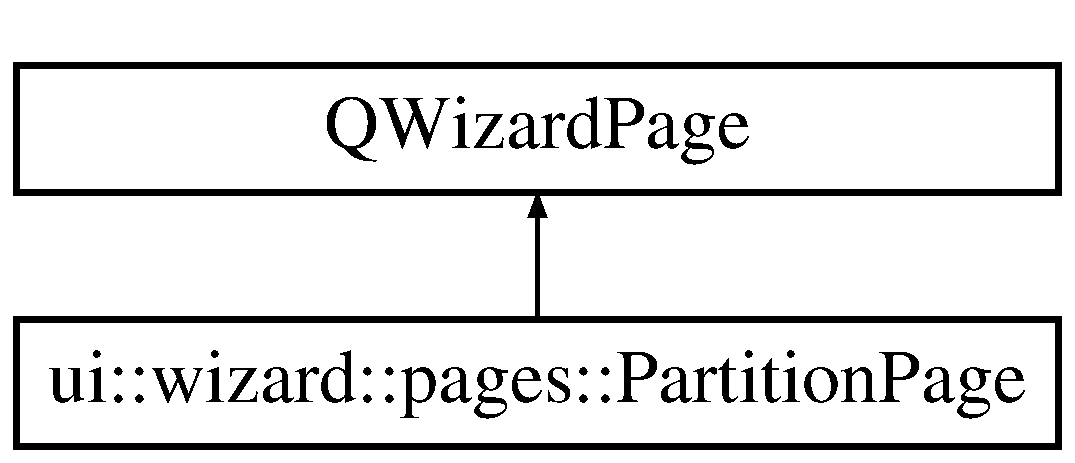
\includegraphics[height=2.000000cm]{classui_1_1wizard_1_1pages_1_1_partition_page}
\end{center}
\end{figure}
\subsection*{Public Slots}
\begin{DoxyCompactItemize}
\item 
void \mbox{\hyperlink{classui_1_1wizard_1_1pages_1_1_partition_page_a0160f5f4dd1dcc377dc7a2f1db732f24}{amount\+Blocks\+Slider\+Value\+Changed}} (int amount)
\begin{DoxyCompactList}\small\item\em amount\+Blocks\+Slider\+Value\+Changed This slot is used to change the value of the partition \end{DoxyCompactList}\item 
void \mbox{\hyperlink{classui_1_1wizard_1_1pages_1_1_partition_page_aa90723be1956b54ce182cc64b3b4ce6f}{block\+Size\+Changed}} (int index)
\begin{DoxyCompactList}\small\item\em block\+Size\+Changed This slot is used to change the block size of the partition \end{DoxyCompactList}\end{DoxyCompactItemize}
\subsection*{Public Member Functions}
\begin{DoxyCompactItemize}
\item 
\mbox{\hyperlink{classui_1_1wizard_1_1pages_1_1_partition_page_a0d12fa168dd41719b3d70cb2effd3629}{Partition\+Page}} (Q\+Widget $\ast$parent=nullptr)
\begin{DoxyCompactList}\small\item\em \mbox{\hyperlink{classui_1_1wizard_1_1pages_1_1_partition_page}{Partition\+Page}} This is a constructor. \end{DoxyCompactList}\item 
virtual \mbox{\hyperlink{classui_1_1wizard_1_1pages_1_1_partition_page_ae74768e1ba91fbf4c094f73ae40ed62c}{$\sim$\+Partition\+Page}} (void) override
\begin{DoxyCompactList}\small\item\em $\sim$\+Partition\+Page Destructor \end{DoxyCompactList}\item 
\mbox{\hyperlink{classui_1_1wizard_1_1pages_1_1_partition_page_a426e777d0785c6992bcfa8a1badd242e}{Partition\+Page}} (unsigned long long \mbox{\hyperlink{classui_1_1wizard_1_1pages_1_1_partition_page_a79050f29e018d84c862fed6fe70bb91c}{disk\+Size}}, Q\+Widget $\ast$parent=nullptr)
\begin{DoxyCompactList}\small\item\em \mbox{\hyperlink{classui_1_1wizard_1_1pages_1_1_partition_page}{Partition\+Page}} This is a constructor. \end{DoxyCompactList}\item 
int \mbox{\hyperlink{classui_1_1wizard_1_1pages_1_1_partition_page_a63ae270155bc6d01ae83adf63860d6f9}{next\+Id}} () const override
\begin{DoxyCompactList}\small\item\em next\+Id This method returns the next id \end{DoxyCompactList}\item 
void \mbox{\hyperlink{classui_1_1wizard_1_1pages_1_1_partition_page_a105573c5cd7af63d8425672c45d2540f}{set\+Visible}} (bool visible) override
\begin{DoxyCompactList}\small\item\em set\+Visible This method toggles the visiblity state of the pages \end{DoxyCompactList}\end{DoxyCompactItemize}
\subsection*{Private Attributes}
\begin{DoxyCompactItemize}
\item 
\mbox{\Hypertarget{classui_1_1wizard_1_1pages_1_1_partition_page_a79050f29e018d84c862fed6fe70bb91c}\label{classui_1_1wizard_1_1pages_1_1_partition_page_a79050f29e018d84c862fed6fe70bb91c}} 
unsigned long long \mbox{\hyperlink{classui_1_1wizard_1_1pages_1_1_partition_page_a79050f29e018d84c862fed6fe70bb91c}{disk\+Size}}
\begin{DoxyCompactList}\small\item\em disk\+Size This attribute state the total usable disk size \end{DoxyCompactList}\item 
\mbox{\Hypertarget{classui_1_1wizard_1_1pages_1_1_partition_page_a62c449957b198f8c748391509bd5ac7a}\label{classui_1_1wizard_1_1pages_1_1_partition_page_a62c449957b198f8c748391509bd5ac7a}} 
Q\+Label $\ast$ \mbox{\hyperlink{classui_1_1wizard_1_1pages_1_1_partition_page_a62c449957b198f8c748391509bd5ac7a}{lb\+Slider\+Value}}
\begin{DoxyCompactList}\small\item\em lb\+Slider\+Value This UI element shows the current value of the slider \end{DoxyCompactList}\item 
\mbox{\Hypertarget{classui_1_1wizard_1_1pages_1_1_partition_page_a0beeb7a451145d8a128160a6ec9a4eef}\label{classui_1_1wizard_1_1pages_1_1_partition_page_a0beeb7a451145d8a128160a6ec9a4eef}} 
Q\+Slider $\ast$ \mbox{\hyperlink{classui_1_1wizard_1_1pages_1_1_partition_page_a0beeb7a451145d8a128160a6ec9a4eef}{slider}}
\begin{DoxyCompactList}\small\item\em slider This UI element changes the partition size \end{DoxyCompactList}\end{DoxyCompactItemize}


\subsection{Detailed Description}
This class provides a custom implementation of a wizard page. 

This class is a custom implementation of a wizard page It request all required information for a partition creation \begin{DoxyAuthor}{Author}
Nils Milewski (10010480) 
\end{DoxyAuthor}


\subsection{Constructor \& Destructor Documentation}
\mbox{\Hypertarget{classui_1_1wizard_1_1pages_1_1_partition_page_a0d12fa168dd41719b3d70cb2effd3629}\label{classui_1_1wizard_1_1pages_1_1_partition_page_a0d12fa168dd41719b3d70cb2effd3629}} 
\index{ui\+::wizard\+::pages\+::\+Partition\+Page@{ui\+::wizard\+::pages\+::\+Partition\+Page}!Partition\+Page@{Partition\+Page}}
\index{Partition\+Page@{Partition\+Page}!ui\+::wizard\+::pages\+::\+Partition\+Page@{ui\+::wizard\+::pages\+::\+Partition\+Page}}
\subsubsection{\texorpdfstring{Partition\+Page()}{PartitionPage()}\hspace{0.1cm}{\footnotesize\ttfamily [1/2]}}
{\footnotesize\ttfamily Partition\+Page\+::\+Partition\+Page (\begin{DoxyParamCaption}\item[{Q\+Widget $\ast$}]{parent = {\ttfamily nullptr} }\end{DoxyParamCaption})}



\mbox{\hyperlink{classui_1_1wizard_1_1pages_1_1_partition_page}{Partition\+Page}} This is a constructor. 

This constructor creates the layout of the page and set required attributes Note only call iff this page is used during a disk creation process 
\begin{DoxyParams}{Parameters}
{\em parent} & Parent object which this object is associated with \\
\hline
\end{DoxyParams}
\mbox{\Hypertarget{classui_1_1wizard_1_1pages_1_1_partition_page_ae74768e1ba91fbf4c094f73ae40ed62c}\label{classui_1_1wizard_1_1pages_1_1_partition_page_ae74768e1ba91fbf4c094f73ae40ed62c}} 
\index{ui\+::wizard\+::pages\+::\+Partition\+Page@{ui\+::wizard\+::pages\+::\+Partition\+Page}!````~Partition\+Page@{$\sim$\+Partition\+Page}}
\index{````~Partition\+Page@{$\sim$\+Partition\+Page}!ui\+::wizard\+::pages\+::\+Partition\+Page@{ui\+::wizard\+::pages\+::\+Partition\+Page}}
\subsubsection{\texorpdfstring{$\sim$\+Partition\+Page()}{~PartitionPage()}}
{\footnotesize\ttfamily Partition\+Page\+::$\sim$\+Partition\+Page (\begin{DoxyParamCaption}\item[{void}]{ }\end{DoxyParamCaption})\hspace{0.3cm}{\ttfamily [override]}, {\ttfamily [virtual]}}



$\sim$\+Partition\+Page Destructor 

This destructor will free up used resources \mbox{\Hypertarget{classui_1_1wizard_1_1pages_1_1_partition_page_a426e777d0785c6992bcfa8a1badd242e}\label{classui_1_1wizard_1_1pages_1_1_partition_page_a426e777d0785c6992bcfa8a1badd242e}} 
\index{ui\+::wizard\+::pages\+::\+Partition\+Page@{ui\+::wizard\+::pages\+::\+Partition\+Page}!Partition\+Page@{Partition\+Page}}
\index{Partition\+Page@{Partition\+Page}!ui\+::wizard\+::pages\+::\+Partition\+Page@{ui\+::wizard\+::pages\+::\+Partition\+Page}}
\subsubsection{\texorpdfstring{Partition\+Page()}{PartitionPage()}\hspace{0.1cm}{\footnotesize\ttfamily [2/2]}}
{\footnotesize\ttfamily Partition\+Page\+::\+Partition\+Page (\begin{DoxyParamCaption}\item[{unsigned long long}]{disk\+Size,  }\item[{Q\+Widget $\ast$}]{parent = {\ttfamily nullptr} }\end{DoxyParamCaption})}



\mbox{\hyperlink{classui_1_1wizard_1_1pages_1_1_partition_page}{Partition\+Page}} This is a constructor. 

This constructor creates the layout of the page and set required attributes, 
\begin{DoxyParams}{Parameters}
{\em disk\+Size} & Size of the disk \\
\hline
{\em parent} & Parent object which this object is associated with \\
\hline
\end{DoxyParams}


\subsection{Member Function Documentation}
\mbox{\Hypertarget{classui_1_1wizard_1_1pages_1_1_partition_page_a0160f5f4dd1dcc377dc7a2f1db732f24}\label{classui_1_1wizard_1_1pages_1_1_partition_page_a0160f5f4dd1dcc377dc7a2f1db732f24}} 
\index{ui\+::wizard\+::pages\+::\+Partition\+Page@{ui\+::wizard\+::pages\+::\+Partition\+Page}!amount\+Blocks\+Slider\+Value\+Changed@{amount\+Blocks\+Slider\+Value\+Changed}}
\index{amount\+Blocks\+Slider\+Value\+Changed@{amount\+Blocks\+Slider\+Value\+Changed}!ui\+::wizard\+::pages\+::\+Partition\+Page@{ui\+::wizard\+::pages\+::\+Partition\+Page}}
\subsubsection{\texorpdfstring{amount\+Blocks\+Slider\+Value\+Changed}{amountBlocksSliderValueChanged}}
{\footnotesize\ttfamily void Partition\+Page\+::amount\+Blocks\+Slider\+Value\+Changed (\begin{DoxyParamCaption}\item[{int}]{amount }\end{DoxyParamCaption})\hspace{0.3cm}{\ttfamily [slot]}}



amount\+Blocks\+Slider\+Value\+Changed This slot is used to change the value of the partition 

This method is invoked if the slider changes his value, inside the method the new partition size will be set 
\begin{DoxyParams}{Parameters}
{\em amount} & Amount of the change \\
\hline
\end{DoxyParams}
\mbox{\Hypertarget{classui_1_1wizard_1_1pages_1_1_partition_page_aa90723be1956b54ce182cc64b3b4ce6f}\label{classui_1_1wizard_1_1pages_1_1_partition_page_aa90723be1956b54ce182cc64b3b4ce6f}} 
\index{ui\+::wizard\+::pages\+::\+Partition\+Page@{ui\+::wizard\+::pages\+::\+Partition\+Page}!block\+Size\+Changed@{block\+Size\+Changed}}
\index{block\+Size\+Changed@{block\+Size\+Changed}!ui\+::wizard\+::pages\+::\+Partition\+Page@{ui\+::wizard\+::pages\+::\+Partition\+Page}}
\subsubsection{\texorpdfstring{block\+Size\+Changed}{blockSizeChanged}}
{\footnotesize\ttfamily void Partition\+Page\+::block\+Size\+Changed (\begin{DoxyParamCaption}\item[{int}]{index }\end{DoxyParamCaption})\hspace{0.3cm}{\ttfamily [slot]}}



block\+Size\+Changed This slot is used to change the block size of the partition 

This method is invoked if the user changes the content of the blocksize combo box, it will set the new block size and adjust the slider max value. 
\begin{DoxyParams}{Parameters}
{\em index} & Index corresponding to block size. 0 = 512, 1 = 1024, 2 = 2048, 3 = 4096, 4 = 8192 \\
\hline
\end{DoxyParams}
\mbox{\Hypertarget{classui_1_1wizard_1_1pages_1_1_partition_page_a63ae270155bc6d01ae83adf63860d6f9}\label{classui_1_1wizard_1_1pages_1_1_partition_page_a63ae270155bc6d01ae83adf63860d6f9}} 
\index{ui\+::wizard\+::pages\+::\+Partition\+Page@{ui\+::wizard\+::pages\+::\+Partition\+Page}!next\+Id@{next\+Id}}
\index{next\+Id@{next\+Id}!ui\+::wizard\+::pages\+::\+Partition\+Page@{ui\+::wizard\+::pages\+::\+Partition\+Page}}
\subsubsection{\texorpdfstring{next\+Id()}{nextId()}}
{\footnotesize\ttfamily int Partition\+Page\+::next\+Id (\begin{DoxyParamCaption}{ }\end{DoxyParamCaption}) const\hspace{0.3cm}{\ttfamily [override]}}



next\+Id This method returns the next id 

This method overrides the default implementation to utilize different intro pages. It will return the enum of next\+\_\+page to differenciate between disk and partition pages \begin{DoxyReturn}{Returns}
Next id for the wizard 
\end{DoxyReturn}
\mbox{\Hypertarget{classui_1_1wizard_1_1pages_1_1_partition_page_a105573c5cd7af63d8425672c45d2540f}\label{classui_1_1wizard_1_1pages_1_1_partition_page_a105573c5cd7af63d8425672c45d2540f}} 
\index{ui\+::wizard\+::pages\+::\+Partition\+Page@{ui\+::wizard\+::pages\+::\+Partition\+Page}!set\+Visible@{set\+Visible}}
\index{set\+Visible@{set\+Visible}!ui\+::wizard\+::pages\+::\+Partition\+Page@{ui\+::wizard\+::pages\+::\+Partition\+Page}}
\subsubsection{\texorpdfstring{set\+Visible()}{setVisible()}}
{\footnotesize\ttfamily void Partition\+Page\+::set\+Visible (\begin{DoxyParamCaption}\item[{bool}]{visible }\end{DoxyParamCaption})\hspace{0.3cm}{\ttfamily [override]}}



set\+Visible This method toggles the visiblity state of the pages 

This method sets the page visible or unset it. It is used to set specific information The page require to operate based on previous information. 
\begin{DoxyParams}{Parameters}
{\em visible} & Visibility state of the page \\
\hline
\end{DoxyParams}


The documentation for this class was generated from the following files\+:\begin{DoxyCompactItemize}
\item 
ui/wizard/pages/partitionpage.\+h\item 
ui/wizard/pages/partitionpage.\+cpp\end{DoxyCompactItemize}

\hypertarget{classui_1_1wizard_1_1_partition_wizard}{}\section{ui\+:\+:wizard\+:\+:Partition\+Wizard Class Reference}
\label{classui_1_1wizard_1_1_partition_wizard}\index{ui\+::wizard\+::\+Partition\+Wizard@{ui\+::wizard\+::\+Partition\+Wizard}}


This class this class implements a wizard.  




{\ttfamily \#include $<$partitionwizard.\+h$>$}

Inheritance diagram for ui\+:\+:wizard\+:\+:Partition\+Wizard\+:\begin{figure}[H]
\begin{center}
\leavevmode
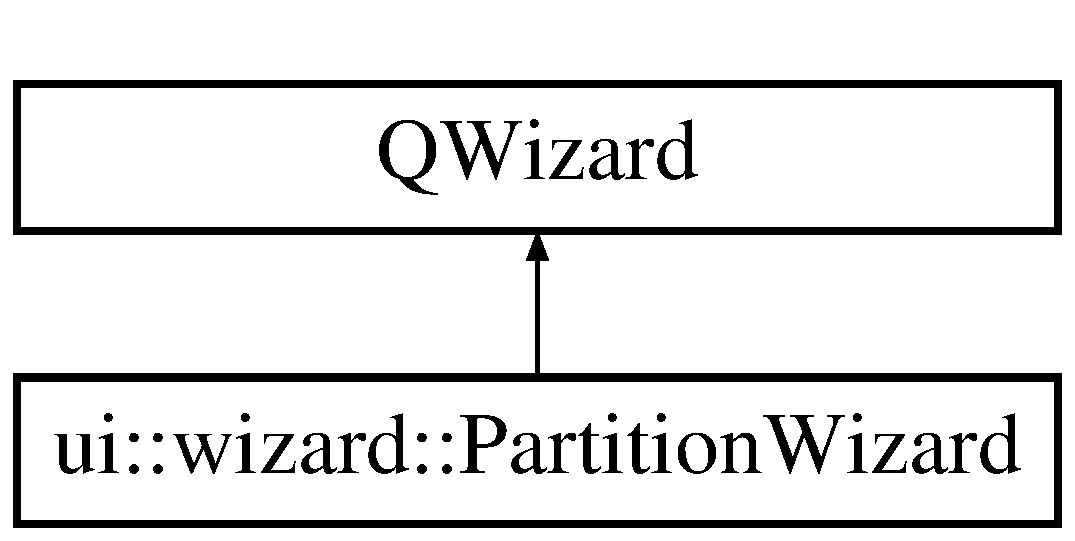
\includegraphics[height=2.000000cm]{classui_1_1wizard_1_1_partition_wizard}
\end{center}
\end{figure}
\subsection*{Public Member Functions}
\begin{DoxyCompactItemize}
\item 
\mbox{\hyperlink{classui_1_1wizard_1_1_partition_wizard_aab98955e5371a971ac94b7f0d4b24258}{Partition\+Wizard}} (unsigned long long disk\+Size, Q\+Widget $\ast$parent=nullptr)
\begin{DoxyCompactList}\small\item\em \mbox{\hyperlink{classui_1_1wizard_1_1_partition_wizard}{Partition\+Wizard}} Constructor. \end{DoxyCompactList}\item 
virtual \mbox{\hyperlink{classui_1_1wizard_1_1_partition_wizard_a356484066944c627c00346690d3ffc80}{$\sim$\+Partition\+Wizard}} (void) override
\begin{DoxyCompactList}\small\item\em $\sim$\+Partition\+Wizard Destructor \end{DoxyCompactList}\item 
\mbox{\hyperlink{classcore_1_1logic_1_1_partition}{core\+::logic\+::\+Partition}} $\ast$ \mbox{\hyperlink{classui_1_1wizard_1_1_partition_wizard_a0ae0814425acc12ed09291de436f8771}{get\+Resulted\+Partition}} (void)
\begin{DoxyCompactList}\small\item\em get\+Resulted\+Partition This method returns the partition which where created. \end{DoxyCompactList}\end{DoxyCompactItemize}
\subsection*{Protected Member Functions}
\begin{DoxyCompactItemize}
\item 
virtual void \mbox{\hyperlink{classui_1_1wizard_1_1_partition_wizard_af5141307f45f8fc9bd091c718a0f31b6}{done}} (int result) override
\begin{DoxyCompactList}\small\item\em done This is a custom implementation of the done event \end{DoxyCompactList}\end{DoxyCompactItemize}


\subsection{Detailed Description}
This class this class implements a wizard. 

This class is a custom implementation of a wizard. It handles all pages and serves as an interaction with the calling object \begin{DoxyAuthor}{Author}
Nils Milewski (10010480) 
\end{DoxyAuthor}


\subsection{Constructor \& Destructor Documentation}
\mbox{\Hypertarget{classui_1_1wizard_1_1_partition_wizard_aab98955e5371a971ac94b7f0d4b24258}\label{classui_1_1wizard_1_1_partition_wizard_aab98955e5371a971ac94b7f0d4b24258}} 
\index{ui\+::wizard\+::\+Partition\+Wizard@{ui\+::wizard\+::\+Partition\+Wizard}!Partition\+Wizard@{Partition\+Wizard}}
\index{Partition\+Wizard@{Partition\+Wizard}!ui\+::wizard\+::\+Partition\+Wizard@{ui\+::wizard\+::\+Partition\+Wizard}}
\subsubsection{\texorpdfstring{Partition\+Wizard()}{PartitionWizard()}}
{\footnotesize\ttfamily Partition\+Wizard\+::\+Partition\+Wizard (\begin{DoxyParamCaption}\item[{unsigned long long}]{disk\+Size,  }\item[{Q\+Widget $\ast$}]{parent = {\ttfamily nullptr} }\end{DoxyParamCaption})}



\mbox{\hyperlink{classui_1_1wizard_1_1_partition_wizard}{Partition\+Wizard}} Constructor. 

This constructor construct a wizard and assign the page order. 
\begin{DoxyParams}{Parameters}
{\em disk\+Size} & Size of the disk where the partition should be created \\
\hline
{\em parent} & \\
\hline
\end{DoxyParams}
\mbox{\Hypertarget{classui_1_1wizard_1_1_partition_wizard_a356484066944c627c00346690d3ffc80}\label{classui_1_1wizard_1_1_partition_wizard_a356484066944c627c00346690d3ffc80}} 
\index{ui\+::wizard\+::\+Partition\+Wizard@{ui\+::wizard\+::\+Partition\+Wizard}!````~Partition\+Wizard@{$\sim$\+Partition\+Wizard}}
\index{````~Partition\+Wizard@{$\sim$\+Partition\+Wizard}!ui\+::wizard\+::\+Partition\+Wizard@{ui\+::wizard\+::\+Partition\+Wizard}}
\subsubsection{\texorpdfstring{$\sim$\+Partition\+Wizard()}{~PartitionWizard()}}
{\footnotesize\ttfamily Partition\+Wizard\+::$\sim$\+Partition\+Wizard (\begin{DoxyParamCaption}\item[{void}]{ }\end{DoxyParamCaption})\hspace{0.3cm}{\ttfamily [override]}, {\ttfamily [virtual]}}



$\sim$\+Partition\+Wizard Destructor 

This destructor will free up used resources 

\subsection{Member Function Documentation}
\mbox{\Hypertarget{classui_1_1wizard_1_1_partition_wizard_af5141307f45f8fc9bd091c718a0f31b6}\label{classui_1_1wizard_1_1_partition_wizard_af5141307f45f8fc9bd091c718a0f31b6}} 
\index{ui\+::wizard\+::\+Partition\+Wizard@{ui\+::wizard\+::\+Partition\+Wizard}!done@{done}}
\index{done@{done}!ui\+::wizard\+::\+Partition\+Wizard@{ui\+::wizard\+::\+Partition\+Wizard}}
\subsubsection{\texorpdfstring{done()}{done()}}
{\footnotesize\ttfamily void Partition\+Wizard\+::done (\begin{DoxyParamCaption}\item[{int}]{result }\end{DoxyParamCaption})\hspace{0.3cm}{\ttfamily [override]}, {\ttfamily [protected]}, {\ttfamily [virtual]}}



done This is a custom implementation of the done event 

This event will ensure that the wizard only closes after the user aproved it with an anwser of a close question. 
\begin{DoxyParams}{Parameters}
{\em result} & Qt internal \\
\hline
\end{DoxyParams}
\mbox{\Hypertarget{classui_1_1wizard_1_1_partition_wizard_a0ae0814425acc12ed09291de436f8771}\label{classui_1_1wizard_1_1_partition_wizard_a0ae0814425acc12ed09291de436f8771}} 
\index{ui\+::wizard\+::\+Partition\+Wizard@{ui\+::wizard\+::\+Partition\+Wizard}!get\+Resulted\+Partition@{get\+Resulted\+Partition}}
\index{get\+Resulted\+Partition@{get\+Resulted\+Partition}!ui\+::wizard\+::\+Partition\+Wizard@{ui\+::wizard\+::\+Partition\+Wizard}}
\subsubsection{\texorpdfstring{get\+Resulted\+Partition()}{getResultedPartition()}}
{\footnotesize\ttfamily \mbox{\hyperlink{classcore_1_1logic_1_1_partition}{core\+::logic\+::\+Partition}} $\ast$ Partition\+Wizard\+::get\+Resulted\+Partition (\begin{DoxyParamCaption}\item[{void}]{ }\end{DoxyParamCaption})}



get\+Resulted\+Partition This method returns the partition which where created. 

This method creates a new partition based on prviouus entered information \begin{DoxyReturn}{Returns}
partition based on previous information 
\end{DoxyReturn}


The documentation for this class was generated from the following files\+:\begin{DoxyCompactItemize}
\item 
ui/wizard/partitionwizard.\+h\item 
ui/wizard/partitionwizard.\+cpp\end{DoxyCompactItemize}

\hypertarget{classui_1_1window_1_1_resize_partition}{}\section{ui\+:\+:window\+:\+:Resize\+Partition Class Reference}
\label{classui_1_1window_1_1_resize_partition}\index{ui\+::window\+::\+Resize\+Partition@{ui\+::window\+::\+Resize\+Partition}}


This class provides a partition resize window.  




{\ttfamily \#include $<$resizepartition.\+h$>$}

Inheritance diagram for ui\+:\+:window\+:\+:Resize\+Partition\+:\begin{figure}[H]
\begin{center}
\leavevmode
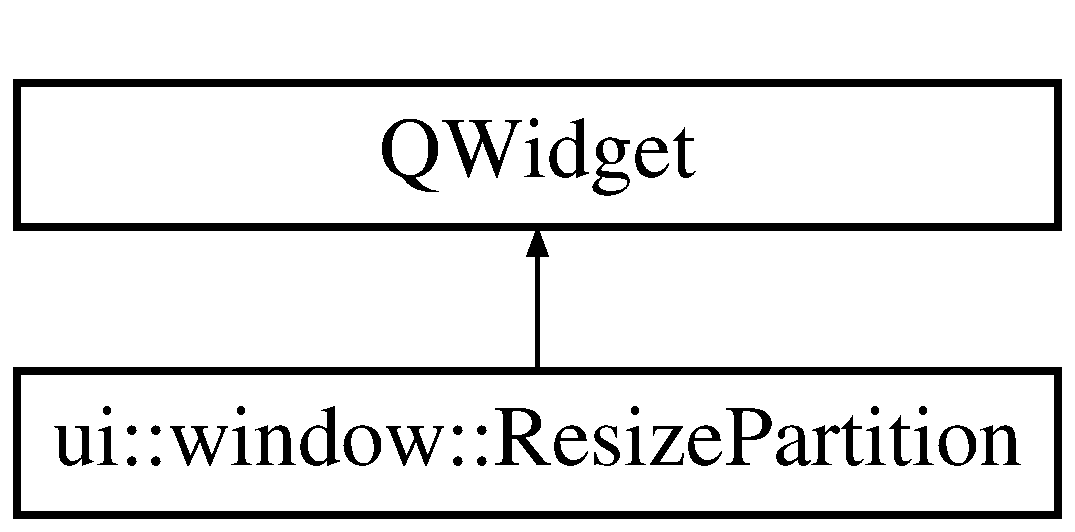
\includegraphics[height=2.000000cm]{classui_1_1window_1_1_resize_partition}
\end{center}
\end{figure}
\subsection*{Public Slots}
\begin{DoxyCompactItemize}
\item 
void \mbox{\hyperlink{classui_1_1window_1_1_resize_partition_a6cdad6be2f435ad46bcf0b537b062a40}{value\+Changed}} (int value)
\begin{DoxyCompactList}\small\item\em value\+Changed This slot is invoked when a slider changes his value \end{DoxyCompactList}\item 
void \mbox{\hyperlink{classui_1_1window_1_1_resize_partition_ab742e4bcdf7e0684ad3e8a787309ef5d}{bt\+Ok\+Pressed}} ()
\begin{DoxyCompactList}\small\item\em bt\+Ok\+Pressed This slot is invoked when a ok button is pressed \end{DoxyCompactList}\item 
void \mbox{\hyperlink{classui_1_1window_1_1_resize_partition_a82f2b0a7f31c72e0ea6176415ddb855c}{bt\+Cancel\+Pressed}} ()
\begin{DoxyCompactList}\small\item\em bt\+Cancel\+Pressed This slot cancels the resize. \end{DoxyCompactList}\end{DoxyCompactItemize}
\subsection*{Public Member Functions}
\begin{DoxyCompactItemize}
\item 
\mbox{\hyperlink{classui_1_1window_1_1_resize_partition_aae9713fef4f920cea006ca9552f02b82}{Resize\+Partition}} (void)
\begin{DoxyCompactList}\small\item\em \mbox{\hyperlink{classui_1_1window_1_1_resize_partition}{Resize\+Partition}} This Cosntructor creates the UI and initializes attributes. \end{DoxyCompactList}\item 
virtual \mbox{\hyperlink{classui_1_1window_1_1_resize_partition_a2e2c8343e7d758f6276ad459424533e9}{$\sim$\+Resize\+Partition}} (void) override
\begin{DoxyCompactList}\small\item\em $\sim$\+Resize\+Partition Destructor \end{DoxyCompactList}\item 
void \mbox{\hyperlink{classui_1_1window_1_1_resize_partition_a1c14acdca1d021b12584b639ac51fc7c}{set\+Disk}} (\mbox{\hyperlink{classcore_1_1disk_1_1_disk}{core\+::disk\+::\+Disk}} $\ast$disk)
\begin{DoxyCompactList}\small\item\em set\+Disk This method sets the working disk \end{DoxyCompactList}\item 
void \mbox{\hyperlink{classui_1_1window_1_1_resize_partition_a0c564d96b48c8c9b134e73184a9f591e}{set\+Index}} (int index)
\begin{DoxyCompactList}\small\item\em set\+Index This method sets the index of the partition \end{DoxyCompactList}\item 
void \mbox{\hyperlink{classui_1_1window_1_1_resize_partition_a3a220945008ce93de147fdf3d8faf486}{show\+Event}} (Q\+Show\+Event $\ast$event) override
\begin{DoxyCompactList}\small\item\em show\+Event This event is called when the window is visible \end{DoxyCompactList}\end{DoxyCompactItemize}
\subsection*{Private Attributes}
\begin{DoxyCompactItemize}
\item 
\mbox{\Hypertarget{classui_1_1window_1_1_resize_partition_ad167e56b7a434144ff8d74b82032eaaa}\label{classui_1_1window_1_1_resize_partition_ad167e56b7a434144ff8d74b82032eaaa}} 
Q\+Label $\ast$ \mbox{\hyperlink{classui_1_1window_1_1_resize_partition_ad167e56b7a434144ff8d74b82032eaaa}{lb\+Max\+Value}}
\begin{DoxyCompactList}\small\item\em max\+Label This UI element displays the maximum space \end{DoxyCompactList}\item 
\mbox{\Hypertarget{classui_1_1window_1_1_resize_partition_ac6bc04608307e6209a7fbf061b02dfe6}\label{classui_1_1window_1_1_resize_partition_ac6bc04608307e6209a7fbf061b02dfe6}} 
Q\+Label $\ast$ \mbox{\hyperlink{classui_1_1window_1_1_resize_partition_ac6bc04608307e6209a7fbf061b02dfe6}{lb\+Current\+Value}}
\begin{DoxyCompactList}\small\item\em current\+Label This UI element displays the current value of the slider \end{DoxyCompactList}\item 
\mbox{\Hypertarget{classui_1_1window_1_1_resize_partition_aa3eacbce4b79f497f9baebdcda9fcf9d}\label{classui_1_1window_1_1_resize_partition_aa3eacbce4b79f497f9baebdcda9fcf9d}} 
Q\+Slider $\ast$ \mbox{\hyperlink{classui_1_1window_1_1_resize_partition_aa3eacbce4b79f497f9baebdcda9fcf9d}{sd\+Partition\+Size}}
\begin{DoxyCompactList}\small\item\em slider This UI element provides the resize functionality \end{DoxyCompactList}\item 
\mbox{\Hypertarget{classui_1_1window_1_1_resize_partition_a8098de513ac511197d124937271850c7}\label{classui_1_1window_1_1_resize_partition_a8098de513ac511197d124937271850c7}} 
Q\+Push\+Button $\ast$ \mbox{\hyperlink{classui_1_1window_1_1_resize_partition_a8098de513ac511197d124937271850c7}{bt\+Ok}}
\begin{DoxyCompactList}\small\item\em bt\+Ok This UI element represents an ok button \end{DoxyCompactList}\item 
\mbox{\Hypertarget{classui_1_1window_1_1_resize_partition_abe84d7ad5ed17041184f17f84e81ed55}\label{classui_1_1window_1_1_resize_partition_abe84d7ad5ed17041184f17f84e81ed55}} 
Q\+Push\+Button $\ast$ \mbox{\hyperlink{classui_1_1window_1_1_resize_partition_abe84d7ad5ed17041184f17f84e81ed55}{bt\+Cancel}}
\begin{DoxyCompactList}\small\item\em bt\+Ok This UI element represents a cancel button \end{DoxyCompactList}\item 
\mbox{\Hypertarget{classui_1_1window_1_1_resize_partition_aa9f3a4abebf2444077705e49ddb3a237}\label{classui_1_1window_1_1_resize_partition_aa9f3a4abebf2444077705e49ddb3a237}} 
\mbox{\hyperlink{classcore_1_1disk_1_1_disk}{core\+::disk\+::\+Disk}} $\ast$ \mbox{\hyperlink{classui_1_1window_1_1_resize_partition_aa9f3a4abebf2444077705e49ddb3a237}{disk\+\_\+m}}
\begin{DoxyCompactList}\small\item\em disk This attribute represent the current working disk \end{DoxyCompactList}\item 
\mbox{\Hypertarget{classui_1_1window_1_1_resize_partition_acde46a28e7bfbfb9750450719e8d8a65}\label{classui_1_1window_1_1_resize_partition_acde46a28e7bfbfb9750450719e8d8a65}} 
int \mbox{\hyperlink{classui_1_1window_1_1_resize_partition_acde46a28e7bfbfb9750450719e8d8a65}{index\+\_\+m}}
\begin{DoxyCompactList}\small\item\em index This attributes is used to detemrine which partition should be resized. \end{DoxyCompactList}\end{DoxyCompactItemize}


\subsection{Detailed Description}
This class provides a partition resize window. 

This class is a window which display the possiblity to resize a partition It will provide a basic layout with the maximum size, minimum size, current size and a slider to adjust the size. \begin{DoxyAuthor}{Author}
Nils Milewski (10010480) 
\end{DoxyAuthor}


\subsection{Constructor \& Destructor Documentation}
\mbox{\Hypertarget{classui_1_1window_1_1_resize_partition_aae9713fef4f920cea006ca9552f02b82}\label{classui_1_1window_1_1_resize_partition_aae9713fef4f920cea006ca9552f02b82}} 
\index{ui\+::window\+::\+Resize\+Partition@{ui\+::window\+::\+Resize\+Partition}!Resize\+Partition@{Resize\+Partition}}
\index{Resize\+Partition@{Resize\+Partition}!ui\+::window\+::\+Resize\+Partition@{ui\+::window\+::\+Resize\+Partition}}
\subsubsection{\texorpdfstring{Resize\+Partition()}{ResizePartition()}}
{\footnotesize\ttfamily Resize\+Partition\+::\+Resize\+Partition (\begin{DoxyParamCaption}\item[{void}]{ }\end{DoxyParamCaption})}



\mbox{\hyperlink{classui_1_1window_1_1_resize_partition}{Resize\+Partition}} This Cosntructor creates the UI and initializes attributes. 

This class requires a partition index corresponding to the partition inside the M\+BR of the disk. 
\begin{DoxyParams}{Parameters}
{\em partition} & Parititon index which should be resized, range 0 -\/ 3. \\
\hline
\end{DoxyParams}
\mbox{\Hypertarget{classui_1_1window_1_1_resize_partition_a2e2c8343e7d758f6276ad459424533e9}\label{classui_1_1window_1_1_resize_partition_a2e2c8343e7d758f6276ad459424533e9}} 
\index{ui\+::window\+::\+Resize\+Partition@{ui\+::window\+::\+Resize\+Partition}!````~Resize\+Partition@{$\sim$\+Resize\+Partition}}
\index{````~Resize\+Partition@{$\sim$\+Resize\+Partition}!ui\+::window\+::\+Resize\+Partition@{ui\+::window\+::\+Resize\+Partition}}
\subsubsection{\texorpdfstring{$\sim$\+Resize\+Partition()}{~ResizePartition()}}
{\footnotesize\ttfamily Resize\+Partition\+::$\sim$\+Resize\+Partition (\begin{DoxyParamCaption}\item[{void}]{ }\end{DoxyParamCaption})\hspace{0.3cm}{\ttfamily [override]}, {\ttfamily [virtual]}}



$\sim$\+Resize\+Partition Destructor 

This destructor will free up used resources 

\subsection{Member Function Documentation}
\mbox{\Hypertarget{classui_1_1window_1_1_resize_partition_a82f2b0a7f31c72e0ea6176415ddb855c}\label{classui_1_1window_1_1_resize_partition_a82f2b0a7f31c72e0ea6176415ddb855c}} 
\index{ui\+::window\+::\+Resize\+Partition@{ui\+::window\+::\+Resize\+Partition}!bt\+Cancel\+Pressed@{bt\+Cancel\+Pressed}}
\index{bt\+Cancel\+Pressed@{bt\+Cancel\+Pressed}!ui\+::window\+::\+Resize\+Partition@{ui\+::window\+::\+Resize\+Partition}}
\subsubsection{\texorpdfstring{bt\+Cancel\+Pressed}{btCancelPressed}}
{\footnotesize\ttfamily void Resize\+Partition\+::bt\+Cancel\+Pressed (\begin{DoxyParamCaption}{ }\end{DoxyParamCaption})\hspace{0.3cm}{\ttfamily [slot]}}



bt\+Cancel\+Pressed This slot cancels the resize. 

This method cancels the resize operation and discards all changes. \mbox{\Hypertarget{classui_1_1window_1_1_resize_partition_ab742e4bcdf7e0684ad3e8a787309ef5d}\label{classui_1_1window_1_1_resize_partition_ab742e4bcdf7e0684ad3e8a787309ef5d}} 
\index{ui\+::window\+::\+Resize\+Partition@{ui\+::window\+::\+Resize\+Partition}!bt\+Ok\+Pressed@{bt\+Ok\+Pressed}}
\index{bt\+Ok\+Pressed@{bt\+Ok\+Pressed}!ui\+::window\+::\+Resize\+Partition@{ui\+::window\+::\+Resize\+Partition}}
\subsubsection{\texorpdfstring{bt\+Ok\+Pressed}{btOkPressed}}
{\footnotesize\ttfamily void Resize\+Partition\+::bt\+Ok\+Pressed (\begin{DoxyParamCaption}{ }\end{DoxyParamCaption})\hspace{0.3cm}{\ttfamily [slot]}}



bt\+Ok\+Pressed This slot is invoked when a ok button is pressed 

This method ensures that all changes from the partition are saved. The partition will shrink or grow after this call \mbox{\Hypertarget{classui_1_1window_1_1_resize_partition_a1c14acdca1d021b12584b639ac51fc7c}\label{classui_1_1window_1_1_resize_partition_a1c14acdca1d021b12584b639ac51fc7c}} 
\index{ui\+::window\+::\+Resize\+Partition@{ui\+::window\+::\+Resize\+Partition}!set\+Disk@{set\+Disk}}
\index{set\+Disk@{set\+Disk}!ui\+::window\+::\+Resize\+Partition@{ui\+::window\+::\+Resize\+Partition}}
\subsubsection{\texorpdfstring{set\+Disk()}{setDisk()}}
{\footnotesize\ttfamily void Resize\+Partition\+::set\+Disk (\begin{DoxyParamCaption}\item[{\mbox{\hyperlink{classcore_1_1disk_1_1_disk}{core\+::disk\+::\+Disk}} $\ast$}]{disk }\end{DoxyParamCaption})}



set\+Disk This method sets the working disk 

This method sets the working disk which the resize operation should be operate on 
\begin{DoxyParams}{Parameters}
{\em disk} & New working disk \\
\hline
\end{DoxyParams}
\mbox{\Hypertarget{classui_1_1window_1_1_resize_partition_a0c564d96b48c8c9b134e73184a9f591e}\label{classui_1_1window_1_1_resize_partition_a0c564d96b48c8c9b134e73184a9f591e}} 
\index{ui\+::window\+::\+Resize\+Partition@{ui\+::window\+::\+Resize\+Partition}!set\+Index@{set\+Index}}
\index{set\+Index@{set\+Index}!ui\+::window\+::\+Resize\+Partition@{ui\+::window\+::\+Resize\+Partition}}
\subsubsection{\texorpdfstring{set\+Index()}{setIndex()}}
{\footnotesize\ttfamily void Resize\+Partition\+::set\+Index (\begin{DoxyParamCaption}\item[{int}]{index }\end{DoxyParamCaption})}



set\+Index This method sets the index of the partition 

This method sets the index which should be used to operate on. Note the partition index must be inside the M\+BR (0 -\/ 3) 
\begin{DoxyParams}{Parameters}
{\em index} & \\
\hline
\end{DoxyParams}
\mbox{\Hypertarget{classui_1_1window_1_1_resize_partition_a3a220945008ce93de147fdf3d8faf486}\label{classui_1_1window_1_1_resize_partition_a3a220945008ce93de147fdf3d8faf486}} 
\index{ui\+::window\+::\+Resize\+Partition@{ui\+::window\+::\+Resize\+Partition}!show\+Event@{show\+Event}}
\index{show\+Event@{show\+Event}!ui\+::window\+::\+Resize\+Partition@{ui\+::window\+::\+Resize\+Partition}}
\subsubsection{\texorpdfstring{show\+Event()}{showEvent()}}
{\footnotesize\ttfamily void Resize\+Partition\+::show\+Event (\begin{DoxyParamCaption}\item[{Q\+Show\+Event $\ast$}]{event }\end{DoxyParamCaption})\hspace{0.3cm}{\ttfamily [override]}}



show\+Event This event is called when the window is visible 

This event occurres if the window enteres the state of visibility. All required field will be set to ensure a acurate functioanlity. 
\begin{DoxyParams}{Parameters}
{\em event} & Qt\+Internal... \\
\hline
\end{DoxyParams}
\mbox{\Hypertarget{classui_1_1window_1_1_resize_partition_a6cdad6be2f435ad46bcf0b537b062a40}\label{classui_1_1window_1_1_resize_partition_a6cdad6be2f435ad46bcf0b537b062a40}} 
\index{ui\+::window\+::\+Resize\+Partition@{ui\+::window\+::\+Resize\+Partition}!value\+Changed@{value\+Changed}}
\index{value\+Changed@{value\+Changed}!ui\+::window\+::\+Resize\+Partition@{ui\+::window\+::\+Resize\+Partition}}
\subsubsection{\texorpdfstring{value\+Changed}{valueChanged}}
{\footnotesize\ttfamily void Resize\+Partition\+::value\+Changed (\begin{DoxyParamCaption}\item[{int}]{value }\end{DoxyParamCaption})\hspace{0.3cm}{\ttfamily [slot]}}



value\+Changed This slot is invoked when a slider changes his value 

When a slider changes hsi value this method will be invoked and refresh the UI 
\begin{DoxyParams}{Parameters}
{\em value} & New slider value \\
\hline
\end{DoxyParams}


The documentation for this class was generated from the following files\+:\begin{DoxyCompactItemize}
\item 
ui/pages/resizepartition.\+h\item 
ui/pages/resizepartition.\+cpp\end{DoxyCompactItemize}

\hypertarget{classui_1_1wizard_1_1pages_1_1_summary_page}{}\section{ui\+:\+:wizard\+:\+:pages\+:\+:Summary\+Page Class Reference}
\label{classui_1_1wizard_1_1pages_1_1_summary_page}\index{ui\+::wizard\+::pages\+::\+Summary\+Page@{ui\+::wizard\+::pages\+::\+Summary\+Page}}


This class provides a custom implementation of a wizard page.  




{\ttfamily \#include $<$summarypage.\+h$>$}

Inheritance diagram for ui\+:\+:wizard\+:\+:pages\+:\+:Summary\+Page\+:\begin{figure}[H]
\begin{center}
\leavevmode
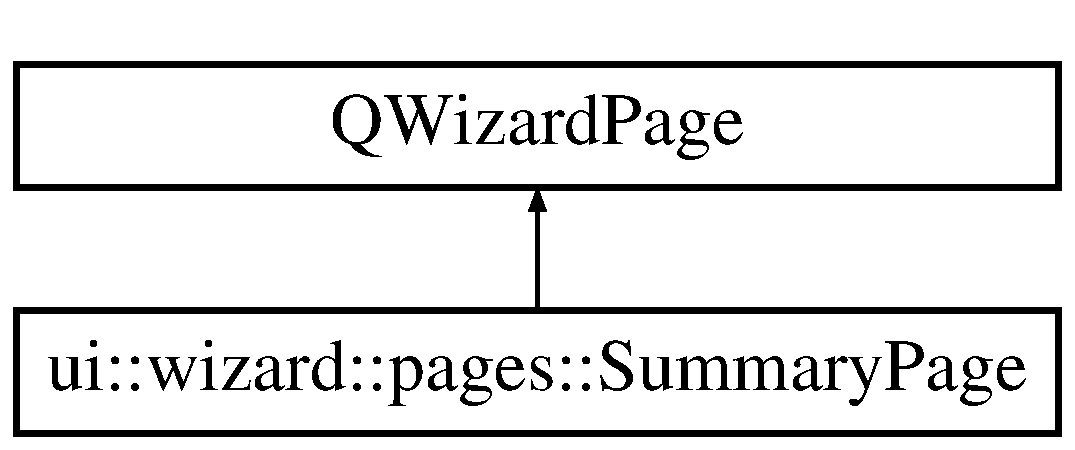
\includegraphics[height=2.000000cm]{classui_1_1wizard_1_1pages_1_1_summary_page}
\end{center}
\end{figure}
\subsection*{Public Member Functions}
\begin{DoxyCompactItemize}
\item 
\mbox{\hyperlink{classui_1_1wizard_1_1pages_1_1_summary_page_a798aff071dddd63b2b5ee049fa87e6a7}{Summary\+Page}} (int used\+Pages, Q\+Widget $\ast$parent=nullptr)
\begin{DoxyCompactList}\small\item\em \mbox{\hyperlink{classui_1_1wizard_1_1pages_1_1_partition_page}{Partition\+Page}} This is a constructor. \end{DoxyCompactList}\item 
virtual \mbox{\hyperlink{classui_1_1wizard_1_1pages_1_1_summary_page_a93b880d988f9f85f28c3d239ce1457e0}{$\sim$\+Summary\+Page}} (void) override
\begin{DoxyCompactList}\small\item\em $\sim$\+Summary\+Page Destructor \end{DoxyCompactList}\end{DoxyCompactItemize}
\subsection*{Protected Member Functions}
\begin{DoxyCompactItemize}
\item 
void \mbox{\hyperlink{classui_1_1wizard_1_1pages_1_1_summary_page_a987e9e51fef71237349acb3b47818737}{initialize\+Page}} () override
\begin{DoxyCompactList}\small\item\em initialize\+Page This method initializes the page \end{DoxyCompactList}\item 
int \mbox{\hyperlink{classui_1_1wizard_1_1pages_1_1_summary_page_a343463680aad6cf8357c9f13fe23e57d}{next\+Id}} () const override
\begin{DoxyCompactList}\small\item\em next\+Id This method returns the next id for the wizard \end{DoxyCompactList}\end{DoxyCompactItemize}
\subsection*{Private Member Functions}
\begin{DoxyCompactItemize}
\item 
Q\+String \mbox{\hyperlink{classui_1_1wizard_1_1pages_1_1_summary_page_af31d12dc5ed2c917c8f65fe7790b661f}{get\+Disk\+Text}} ()
\begin{DoxyCompactList}\small\item\em get\+Disk\+Text This method returns a text representing a disk \end{DoxyCompactList}\item 
Q\+String \mbox{\hyperlink{classui_1_1wizard_1_1pages_1_1_summary_page_a0100c8e2a029708c5447c20c83bd7257}{get\+Partitio\+N\+Text}} ()
\begin{DoxyCompactList}\small\item\em get\+Partitio\+N\+Text This method returns a text representing a partition \end{DoxyCompactList}\end{DoxyCompactItemize}
\subsection*{Private Attributes}
\begin{DoxyCompactItemize}
\item 
int \mbox{\hyperlink{classui_1_1wizard_1_1pages_1_1_summary_page_a8e0bd026c5d978fbb1bf157439867fd5}{used\+Pages\+\_\+m}}
\begin{DoxyCompactList}\small\item\em used\+Pages This variable defines which pages was shown to the user \end{DoxyCompactList}\end{DoxyCompactItemize}


\subsection{Detailed Description}
This class provides a custom implementation of a wizard page. 

This class is a custom implementation of a wizard page It displays all information which where previous entered. \begin{DoxyAuthor}{Author}
Nils Milewski (10010480) 
\end{DoxyAuthor}


\subsection{Constructor \& Destructor Documentation}
\mbox{\Hypertarget{classui_1_1wizard_1_1pages_1_1_summary_page_a798aff071dddd63b2b5ee049fa87e6a7}\label{classui_1_1wizard_1_1pages_1_1_summary_page_a798aff071dddd63b2b5ee049fa87e6a7}} 
\index{ui\+::wizard\+::pages\+::\+Summary\+Page@{ui\+::wizard\+::pages\+::\+Summary\+Page}!Summary\+Page@{Summary\+Page}}
\index{Summary\+Page@{Summary\+Page}!ui\+::wizard\+::pages\+::\+Summary\+Page@{ui\+::wizard\+::pages\+::\+Summary\+Page}}
\subsubsection{\texorpdfstring{Summary\+Page()}{SummaryPage()}}
{\footnotesize\ttfamily Summary\+Page\+::\+Summary\+Page (\begin{DoxyParamCaption}\item[{int}]{used\+Pages,  }\item[{Q\+Widget $\ast$}]{parent = {\ttfamily nullptr} }\end{DoxyParamCaption})}



\mbox{\hyperlink{classui_1_1wizard_1_1pages_1_1_partition_page}{Partition\+Page}} This is a constructor. 

This constructor creates the layout of the page 
\begin{DoxyParams}{Parameters}
{\em parent} & Parent object which this object is associated with \\
\hline
\end{DoxyParams}
\mbox{\Hypertarget{classui_1_1wizard_1_1pages_1_1_summary_page_a93b880d988f9f85f28c3d239ce1457e0}\label{classui_1_1wizard_1_1pages_1_1_summary_page_a93b880d988f9f85f28c3d239ce1457e0}} 
\index{ui\+::wizard\+::pages\+::\+Summary\+Page@{ui\+::wizard\+::pages\+::\+Summary\+Page}!````~Summary\+Page@{$\sim$\+Summary\+Page}}
\index{````~Summary\+Page@{$\sim$\+Summary\+Page}!ui\+::wizard\+::pages\+::\+Summary\+Page@{ui\+::wizard\+::pages\+::\+Summary\+Page}}
\subsubsection{\texorpdfstring{$\sim$\+Summary\+Page()}{~SummaryPage()}}
{\footnotesize\ttfamily Summary\+Page\+::$\sim$\+Summary\+Page (\begin{DoxyParamCaption}\item[{void}]{ }\end{DoxyParamCaption})\hspace{0.3cm}{\ttfamily [override]}, {\ttfamily [virtual]}}



$\sim$\+Summary\+Page Destructor 

This destructor will free up used resources 

\subsection{Member Function Documentation}
\mbox{\Hypertarget{classui_1_1wizard_1_1pages_1_1_summary_page_af31d12dc5ed2c917c8f65fe7790b661f}\label{classui_1_1wizard_1_1pages_1_1_summary_page_af31d12dc5ed2c917c8f65fe7790b661f}} 
\index{ui\+::wizard\+::pages\+::\+Summary\+Page@{ui\+::wizard\+::pages\+::\+Summary\+Page}!get\+Disk\+Text@{get\+Disk\+Text}}
\index{get\+Disk\+Text@{get\+Disk\+Text}!ui\+::wizard\+::pages\+::\+Summary\+Page@{ui\+::wizard\+::pages\+::\+Summary\+Page}}
\subsubsection{\texorpdfstring{get\+Disk\+Text()}{getDiskText()}}
{\footnotesize\ttfamily Q\+String Summary\+Page\+::get\+Disk\+Text (\begin{DoxyParamCaption}{ }\end{DoxyParamCaption})\hspace{0.3cm}{\ttfamily [private]}}



get\+Disk\+Text This method returns a text representing a disk 

This method querries all attributes of a disk and creates a human readable string which can be used to display disk inormation \begin{DoxyReturn}{Returns}
Summary of disk in string format 
\end{DoxyReturn}
\mbox{\Hypertarget{classui_1_1wizard_1_1pages_1_1_summary_page_a0100c8e2a029708c5447c20c83bd7257}\label{classui_1_1wizard_1_1pages_1_1_summary_page_a0100c8e2a029708c5447c20c83bd7257}} 
\index{ui\+::wizard\+::pages\+::\+Summary\+Page@{ui\+::wizard\+::pages\+::\+Summary\+Page}!get\+Partitio\+N\+Text@{get\+Partitio\+N\+Text}}
\index{get\+Partitio\+N\+Text@{get\+Partitio\+N\+Text}!ui\+::wizard\+::pages\+::\+Summary\+Page@{ui\+::wizard\+::pages\+::\+Summary\+Page}}
\subsubsection{\texorpdfstring{get\+Partitio\+N\+Text()}{getPartitioNText()}}
{\footnotesize\ttfamily Q\+String Summary\+Page\+::get\+Partitio\+N\+Text (\begin{DoxyParamCaption}{ }\end{DoxyParamCaption})\hspace{0.3cm}{\ttfamily [private]}}



get\+Partitio\+N\+Text This method returns a text representing a partition 

This method querries all attributes of a partition and creates a human readable string which can be used to display disk inormation \begin{DoxyReturn}{Returns}
Summary of partition in string format 
\end{DoxyReturn}
\mbox{\Hypertarget{classui_1_1wizard_1_1pages_1_1_summary_page_a987e9e51fef71237349acb3b47818737}\label{classui_1_1wizard_1_1pages_1_1_summary_page_a987e9e51fef71237349acb3b47818737}} 
\index{ui\+::wizard\+::pages\+::\+Summary\+Page@{ui\+::wizard\+::pages\+::\+Summary\+Page}!initialize\+Page@{initialize\+Page}}
\index{initialize\+Page@{initialize\+Page}!ui\+::wizard\+::pages\+::\+Summary\+Page@{ui\+::wizard\+::pages\+::\+Summary\+Page}}
\subsubsection{\texorpdfstring{initialize\+Page()}{initializePage()}}
{\footnotesize\ttfamily void Summary\+Page\+::initialize\+Page (\begin{DoxyParamCaption}{ }\end{DoxyParamCaption})\hspace{0.3cm}{\ttfamily [override]}, {\ttfamily [protected]}}



initialize\+Page This method initializes the page 

This method overrides the base initialize\+Page method to ensure that Custom behaivour can be implemented. This method sets the subtitle with all previous entered information \mbox{\Hypertarget{classui_1_1wizard_1_1pages_1_1_summary_page_a343463680aad6cf8357c9f13fe23e57d}\label{classui_1_1wizard_1_1pages_1_1_summary_page_a343463680aad6cf8357c9f13fe23e57d}} 
\index{ui\+::wizard\+::pages\+::\+Summary\+Page@{ui\+::wizard\+::pages\+::\+Summary\+Page}!next\+Id@{next\+Id}}
\index{next\+Id@{next\+Id}!ui\+::wizard\+::pages\+::\+Summary\+Page@{ui\+::wizard\+::pages\+::\+Summary\+Page}}
\subsubsection{\texorpdfstring{next\+Id()}{nextId()}}
{\footnotesize\ttfamily int Summary\+Page\+::next\+Id (\begin{DoxyParamCaption}{ }\end{DoxyParamCaption}) const\hspace{0.3cm}{\ttfamily [override]}, {\ttfamily [protected]}}



next\+Id This method returns the next id for the wizard 

This method overrides the default implementation to ensure a dynamic wizard. This page will allways return -\/1 to signal a final page. \begin{DoxyReturn}{Returns}
next wizard ID 
\end{DoxyReturn}


\subsection{Member Data Documentation}
\mbox{\Hypertarget{classui_1_1wizard_1_1pages_1_1_summary_page_a8e0bd026c5d978fbb1bf157439867fd5}\label{classui_1_1wizard_1_1pages_1_1_summary_page_a8e0bd026c5d978fbb1bf157439867fd5}} 
\index{ui\+::wizard\+::pages\+::\+Summary\+Page@{ui\+::wizard\+::pages\+::\+Summary\+Page}!used\+Pages\+\_\+m@{used\+Pages\+\_\+m}}
\index{used\+Pages\+\_\+m@{used\+Pages\+\_\+m}!ui\+::wizard\+::pages\+::\+Summary\+Page@{ui\+::wizard\+::pages\+::\+Summary\+Page}}
\subsubsection{\texorpdfstring{used\+Pages\+\_\+m}{usedPages\_m}}
{\footnotesize\ttfamily int ui\+::wizard\+::pages\+::\+Summary\+Page\+::used\+Pages\+\_\+m\hspace{0.3cm}{\ttfamily [private]}}



used\+Pages This variable defines which pages was shown to the user 

This variable is used to determine which information will be displayed to the user 

The documentation for this class was generated from the following files\+:\begin{DoxyCompactItemize}
\item 
ui/wizard/pages/summarypage.\+h\item 
ui/wizard/pages/summarypage.\+cpp\end{DoxyCompactItemize}

%--- End generated contents ---

% Index
\backmatter
\newpage
\phantomsection
\clearemptydoublepage
\addcontentsline{toc}{chapter}{Index}
\printindex

\end{document}
